\chapter{Core Theories}\label{HOLtheories}

% LaTeX macros in HOL manuals
%
% \holtxt{..}     for typewriter text that is HOL types or terms.  To
%                 produce backslashes, for /\, \/ and \x. x + 1, use \bs
% \ml{..}         for typewriter text that is ML input, including the
%                 names of HOL API functions, such as mk_const
% \theoryimp{..}  for names of HOL theories.

% Inside \begin{verbatim}, indent contents three spaces, unless
% displaying a HOL session in a box (boxed or session environments).
% In that case, put the session flush against the left margin

% Rather than wrapping begin{verbatim} blocks in \small, which does
% terrible things to line-spacing in the vicinity, use the hol
% environment, thus \begin{hol}\begin{verbatim}...\end{verbatim}\end{hol}

\setcounter{sessioncount}{0}


\newcommand{\konst}[1]{\ensuremath{\mbox{\small{\textbf{\sf{#1}}}}}}
\newcommand{\nil}{\mathbf{[} \;\mathbf{]}}
\newcommand{\cons}[2]{{#1}\mathbf{:}\mathbf{:}{#2}}

\index{theories, in HOL logic@theories, in \HOL{} logic!hierarchies
of}%
The \HOL{} system provides a collection of theories on which to base verification tools or further theory development.
In the rest of this section, these theories are briefly described.
The sections that follow provide an overview of the contents of each theory.
For a complete list of all the axioms, definitions and theorems in \HOL, see the online resources distributed with the system.
In particular, the HTML file \url{help/HOLindex.html} is a good place to start browsing the available theories.
For a graphical picture of the theory hierarchy, see \url{help/theorygraph/theories.html}.

\section{The Theory {\tt min}}\label{minTheory}

The starting theory of \HOL{} is the theory \ml{min}.
\index{min, the HOL theory@\ml{min}, the \HOL{} theory|(}
In this theory, the type constant {\small\verb+bool+} of booleans,
the binary type operator $(\alpha,\beta)${\small\verb+fun+} of functions, and the type
constant {\small\verb+ind+} of individuals are declared. Building on
these types, three primitive constants
\index{constants, in HOL logic@constants, in \HOL{} logic!primitive logical}%
\index{primitive constants, of HOL logic@primitive constants, of \HOL{} logic}%
are declared: equality, implication, and a choice operator:
\index{ equality, in HOL logic@\ml{=} (equality, in \HOL{} logic)}
\index{equality, in HOL logic@equality, in \HOL{} logic}
\begin{description}
\item [Equality] Equality ({\small\verb+= : 'a -> 'a -> bool+}) is an
  infix operator.
\index{equality, in HOL logic@equality, in \HOL{} logic}
\item [Implication] Implication
  ({\small\verb+==> : bool -> bool -> bool+}) is the
  \emph{material implication} and is an infix operator that is
  right-associative, \ie, \verb+x ==> y ==> z+ parses to the same term
  as \verb+x ==> (y ==> z)+.
\index{implication, in HOL logic@implication, in \HOL{} logic}
\item [Choice] Equality
and implication are standard predicate calculus notions, but choice is
more exotic: if $t$ is a term having type $\sigma${\small\verb+->bool+},
then {\small\verb+@x.+}$t${\small\verb+ x+} (or, equivalently,
{\small\verb+$@+}$t$) denotes \emph{some} member of the set whose
characteristic\index{characteristic predicate, of type definitions}
 function is $t$. If the set is empty, then
{\small\verb+@x.+}$t${\small\verb+ x+} denotes an arbitrary member of the
set denoted by $\sigma$. The constant {\small\verb+@+} is a higher order
version of Hilbert's
\index{Hilbert, D.}%
\index{epsilon operator}%
 $\hilbert$-operator; it is related to the constant
$\iota$ in Church's formulation of higher order logic. For more details,
see Church's
\index{Church, A.}
original paper \cite{Church}, Leisenring's
\index{Leisenring, A.}
book on Hilbert's $\hilbert$-symbol \cite{Leisenring}, or Andrews'
textbook on type theory \cite{Andrews}.
\end{description}

\medskip

\noindent No theorems or axioms are placed in theory \theoryimp{min}.
The primitive rules of inference of \HOL{} depend on the presence of
\theoryimp{min}.
%
\index{min, the HOL theory@\ml{min}, the \HOL{} theory|)}

\section{Basic Theories}

The most basic theories in HOL provide support for a standard
collection of types. The theory \theoryimp{bool} defines the basis of
the \HOL{} logic, including the boolean operations and
quantifiers. On this platform, quite a bit of theorem-proving
infrastructure can already be built. Further basic types are developed
in the theory of pairs (\theoryimp{prod}), disjoint sums
(\theoryimp{sum}), the one-element type (\theoryimp{one}), and the
(\theoryimp{option}) type.


\subsection{The theory \theoryimp{bool}}\label{boolfull}

\index{axioms!primitive, of HOL logic@primitive, of \HOL{} logic|(}
%
At start-up, the initial theory for users of the \HOL{} system is
called \ml{bool}\index{HOL@\HOL{}}, which is constructed when the
\HOL{} system is built. The theory \theoryimp{bool} is an extension of
the combination of the ``conceptual'' theories \theory{LOG} and
\theory{INIT}, described in \LOGIC.  Thus it contains the four axioms
%
\index{axioms!in bool theory@in \ml{bool} theory}
%
for higher order logic. These axioms, together with the rules of
inference described in Section~\ref{rules}, constitute the core of the
\HOL{} logic.  Because of the way the \HOL{} system evolved from \LCF%
%
\index{LCF@\LCF}%
%
\footnote{To simplify the porting of the LCF theorem-proving tools to
  the HOL system, the HOL logic was made as like PP$\lambda$ (the
  logic built-in to LCF) as possible.}, the particular axiomatization
of higher order logic it uses differs from the classical
axiomatization due to Church\index{Church, A.}  \cite{Church}.  The
biggest difference is that in Church's formulation type variables
%
\index{type variables, in HOL logic@type variables, in \HOL{} logic!differences from classical}
%
are in the meta-language, whereas in the \HOL{} logic they are part of
the object language.

The logical constants
%
\index{logical constants, in HOL logic@logical constants, in \HOL{} logic}
%
\holtxt{T}~(truth),
%
\index{truth values, in HOL logic@truth values, in \HOL{} logic!constants for}
%
\holtxt{F}~(falsity),
\holtxt{\~{}}~(negation),
%
\index{ negation, in HOL logic@\holtxt{\~{}} (negation, in \HOL{} logic)}
%
\holtxt{/\bs} (conjunction),
%
\index{ conjunction, in HOL logic@\holtxt{/\bs} (conjunction, in \HOL{} logic)}
%
\holtxt{\bs/} (disjunction),
%
\index{ disjunction, in HOL logic@\holtxt{\bs/} (disjunction, in \HOL{} logic)}
%
\holtxt{!} (universal quantification),
%
\index{ universal quantifier, in HOL logic@\holtxt{"!} (universal quantifier, in \HOL{} logic)}
%
\holtxt{?} (existential quantification),
%
\index{ existential quantifier, in HOL logic@\holtxt{?} (existential quantifier, in \HOL{} logic)}
%
and \holtxt{?!} (unique existence quantifier)
%
\index{ exists unique, in HOL logic@\holtxt{?"!} (exists unique, in \HOL{} logic)}
%
can all be defined in terms of equality,
%
\index{equality, in HOL logic@equality, in \HOL{} logic}
%
implication and choice.  The definitions listed below are fairly
standard; each one is preceded by its \ML{} name.  Later definitions
sometimes build on earlier ones.

\begin{hol}
\index{truth values, in HOL logic@truth values, in \HOL{} logic!definition of}
\index{T@\holtxt{T}!definitional axiom for}
\index{disjunction, in HOL logic@disjunction, in \HOL{} logic!definitional axiom for}
\index{conjunction, in HOL logic@conjunction, in \HOL{} logic!definitional axiom for}
\index{iff, in HOL logic@iff, in \HOL{} logic!definitional axiom for}
\index{negation, in HOL logic@negation, in \HOL{} logic!definitional axiom for}
\index{ exists unique, in HOL logic@\holtxt{?"!} (exists unique, in \HOL{} logic)}
\index{F (falsity), the HOL constant@\holtxt{F} (falsity), the \HOL{} constant!definitional axiom for}
\index{conjunction, in HOL logic@conjunction, in \HOL{} logic!definitional axiom for}
\index{disjunction, in HOL logic@disjunction, in \HOL{} logic!definitional axiom for}
\index{equality, in HOL logic@equality, in \HOL{} logic!primitive axiom for}
\index{existential quantifier, in HOL logic@existential quantifier, in \HOL{} logic!definitional axiom for}
\index{universal quantifier, in HOL logic@universal quantifier, in \HOL{} logic!definitional axiom for}
\index{exists unique, in HOL logic@exists unique, in \HOL{} logic!definitional axiom for}
\begin{verbatim}
   T_DEF              |- T  = ((\x:bool. x) = (\x. x))

   FORALL_DEF         |- !  = \P:'a->bool. P = (\x. T)

   EXISTS_DEF         |- ?  = \P:'a->bool. P($@ P)

   AND_DEF            |- /\ = \t1 t2. !t. (t1 ==> t2 ==> t) ==> t

   OR_DEF             |- \/ = \t1 t2. !t. (t1 ==> t) ==> (t2 ==> t) ==> t

   F_DEF              |- F  = !t. t

   NOT_DEF            |- ~  = (\t. t ==> F)

   EXISTS_UNIQUE_DEF  |- ?! = (\P. $? P /\ (!x y. P x /\ P y ==> (x = y)))
\end{verbatim}
\end{hol}


There are four
%
\index{universal quantifier, in HOL logic@universal quantifier, in \HOL{} logic!in four primitive axioms}
%
axioms in the theory \theoryimp{bool};
%
\index{bool, the HOL theory@\ml{bool}, the \HOL{} theory}
%
the first three are the following:

\begin{hol}
\index{BOOL_CASES_AX@\ml{BOOL\_CASES\_AX}}
\index{ETA_AX@\ml{ETA\_AX}}
\index{SELECT_AX@\ml{SELECT\_AX}}
\index{implication, in HOL logic@implication, in \HOL{} logic!primitive axiom for}
\index{ choice function, in HOL logic@\holtxt{"@} (choice function, in \HOL{} logic)}
\index{choice axiom}
\index{axiom of choice}
\index{axioms!of choice}
\index{choice operator, in HOL logic@choice operator, in \HOL{} logic!primitive axiom for}
\begin{verbatim}
   BOOL_CASES_AX   |- !t. (t = T) \/ (t = F)

   ETA_AX          |- !t. (\x. t x) = t

   SELECT_AX       |- !P:'a->bool x. P x ==> P($@ P)
\end{verbatim}
\end{hol}

\noindent
The fourth and last axiom of the \HOL{} logic is the Axiom of
Infinity\index{axiom of infinity}. Its statement is phrased in terms of
the function properties {\small\verb+ONE_ONE+} and {\small\verb+ONTO+}. The
definitions are:

\begin{hol}
\index{ONE_ONE_DEF@\ml{ONE\_ONE\_DEF}}
\index{ONTO_DEF@\ml{ONTO\_DEF}}
\index{one-to-one predicate, in HOL logic@one-to-one predicate, in \HOL{} logic!definitional axiom for}
\index{onto predicate, in HOL logic@onto predicate, in \HOL{} logic!definitional axiom for}
\begin{verbatim}
   ONE_ONE_DEF |- ONE_ONE f = (!x1 x2. (f x1 = f x2) ==> (x1 = x2))

   ONTO_DEF    |- ONTO f    = (!y. ?x. y = f x)
\end{verbatim}
\end{hol}

\noindent The Axiom of Infinity\index{axioms!in bool theory@in \ml{bool} theory} is
%
\begin{hol}
\index{INFINITY_AX@\ml{INFINITY\_AX}}
\index{axiom of infinity}
\index{existential quantifier, in HOL logic@existential quantifier, in \HOL{} logic!in infinity axiom}
\begin{verbatim}
  INFINITY_AX  |- ?f:ind->ind. ONE_ONE f /\ ~(ONTO f)
\end{verbatim}
\end{hol}
%
\noindent
This asserts that there exists a one-to-one map from \holtxt{ind} to
itself that is not onto. This implies that the type \holtxt{ind}
denotes an infinite set.
%
\index{axioms!primitive, of HOL logic@primitive, of \HOL{} logic|)}

The three other axioms of the theory \theoryimp{bool}, the rules of
inference in Section~\ref{rules} and the Axiom of Infinity are,
together, sufficient for developing all of standard mathematics. Thus,
in principle, the user of the \HOL{} system should never need to make a
non-definitional
%
\index{axioms!dispensibility of adding}%
\index{definitional theories}%
%
theory. In practice, it is often very tempting to take the risk of
introducing new axioms because deriving them from definitions can be
tedious---proving that `axioms' follow from definitions amounts to
proving their consistency.

\paragraph {Further definitions}

The theory \theoryimp{bool} also supplies the definitions of a number of
useful constants.
\begin{hol}
\index{COND, the HOL constant@\holtxt{COND}, the \HOL{} constant}
\index{LET, the HOL constant@\ml{LET}, the \HOL{} constant}
\index{conditionals, in HOL logic@conditionals, in \HOL{} logic!definitional axiom for}
\begin{verbatim}
   LET_DEF  |- LET  = \f x. f x
   COND_DEF |- COND = \t t1 t2. @x. ((t=T)==>(x=t1)) /\ ((t=F)==>(x=t2))
   IN_DEF   |- IN   = \x (f:'a -> bool). f x
\end{verbatim}
\end{hol}

The constant \holtxt{LET}
%
\index{let-terms, in HOL logic@\holtxt{let}-terms, in \HOL{} logic!constant for}
%
is used in representing terms containing local variable bindings (\ie\
\holtxt{let}-terms).
%
\index{let-terms, in HOL logic@\holtxt{let}-terms, in \HOL{} logic!definitional axiom for}
%
For example, the concrete syntax \holtxt{let v = M in N} is translated
by the parser to the term \holtxt{LET (\bs{}v.N) M}. For the full
description of how \holtxt{let} expressions are translated, see
Section \ref{prod}.

The constant \holtxt{COND} is used to represent conditional
expressions. The concrete syntax
%
\index{terms, in HOL logic@terms, in \HOL{} logic!conditional}%
\index{conditionals, in HOL logic@conditionals, in \HOL{} logic}%
%
$\holtxt{if}\;t_1\;\holtxt{then}\;t_2\;\holtxt{else}\;t_3$ abbreviates
the application \holtxt{COND $t_1$ $t_2$ $t_3$}.

The constant \holtxt{IN} (written as an infix) is the basis of
the modelling of sets by their characteristic functions.  The term
$x\holtxt{ IN }P$ can be read as ``$x$ is an element of the set
$P$'', or (more in line with its definition) as ``the predicate $P$ is
true of $x$''.

Finally, the polymorphic constant $\holtxt{ARB}:\alpha$ denotes a
fixed but arbitrary element. \holtxt{ARB} is occasionally useful when
attempting to deal with the issue of partiality.

\subsubsection{Restricted quantifiers}\label{res-quant}

\index{restricted quantification}
%
The theory \theoryimp{bool} also defines constants that implement
\emph{restricted quantification}. This provides a means of simulating
subtypes and dependent types with predicates. The most heavily used
are restrictions of the existential and universal quantifiers:
%
\begin{verbatim}
   RES_FORALL_DEF |- RES_FORALL = \P m. !x. x IN P ==> m x

   RES_EXISTS_DEF |- RES_EXISTS = \P m. ?x. x IN P /\ m x

   RES_ABSTRACT_DEF |- (!P m x. x IN P ==> (RES_ABSTRACT P m x = m x) /\
                       (!P m1 m2.
                           (!x. x IN P ==> (m1 x = m2 x)) ==>
                            (RES_ABSTRACT P m1 = RES_ABSTRACT P m2)
\end{verbatim}
%
The definition of \ml{RES\_ABSTRACT} is a characterising formula, rather
than a direct equation.  There are two important properties
\begin{itemize}
\item if $y$ is an element of $P$ then $(\bs{}x :: P.\; M)
  y = M[y/x]$
\item If two restricted abstractions agree on all values over their
  (common) restricting set, then they are equal.
\end{itemize}

For completeness, restricted versions of unique existence and
indefinite description are provided, although hardly used.
\begin{verbatim}
   RES_EXISTS_UNIQUE_DEF
    |- RES_EXISTS_UNIQUE = \P m. (?x :: P. m x) /\
                                 (!x y :: P. m x /\ m y ==> (x = y))

   RES_SELECT_DEF
     |- RES_SELECT = \P m. @x. x IN P /\ m x
\end{verbatim}

The definition of \ml{RES\_EXISTS\_UNIQUE} uses the restricted
quantification syntax with the {\small\verb+::+} symbol, referring to
the earlier definitions \ml{RES\_EXISTS} and \ml{RES\_FORALL}.
The \texttt{::} syntax is used with restricted quantifiers to allow
arbitrary predicates to restrict binding variables. The \HOL{} parser
allows restricted quantification of all of a sequence of binding
variables by putting the restriction at the end of the sequence, thus
with a universal quantification:
%
\[
\forall x \, y \, z \, {\tt ::} \; P \, . \; Q(x,y,z)
\]
%
Here the predicate $P$ restricts all of $x$, $y$ and $z$.

\subsubsection{Derived syntactic forms}\label{derived-terms}

\index{quotation, in HOL logic@quotation, in \HOL{} logic!of non-primitive terms|(}
% don't refill the \index entries above, it's important to keep each
% entry on one line
The \HOL{} quotation parser
%
\index{quotation, in HOL logic@quotation, in \HOL{} logic!parser for}
%
can translate various standard logical
notations
%
\index{parsing, of HOL logic@parsing, of \HOL{} logic!of standard notations}
%
into primitive terms. For example, if \ml{+} has been declared an
infix
%
\index{infixes, in HOL logic@infixes, in \HOL{} logic}
%
(as explained in Section~\ref{theoryfns}), as it is when
\ml{arithmeticTheory} has been loaded, then \ml{``x+1``} is
translated to \ml{``\$+~x~1``}. The escape character \ml{\$}
%
\index{ escape, in HOL logic parser@\ml{\$} (escape, in \HOL{} logic parser)}%
\index{declared constants, in HOL logic@declared constants, in \HOL{} logic}%
\index{infixes, in HOL logic@infixes, in \HOL{} logic}%
%
suppresses the infix behaviour of \ml{+} and prevents the quotation
parser getting confused.  In general, \ml{\$} can be used to suppress
any special syntactic behaviour a token (such as \texttt{if},
\texttt{+} or \texttt{let})
%
\index{tokens!suppressing parsing behaviour of}
%
might have. This is illustrated in the table below, in which the terms
in the column headed \textit{`\ML{} quotation'} are translated by the
quotation parser to the corresponding terms in the column headed
\textit{`Primitive term'}.  Conversely, the terms in the latter column
are always printed in the form shown in the former one.  The \ML{}
constructor expressions in the rightmost column evaluate to the same
values (of type \ml{term}) as the other quotations in the same row.

\bigskip

\begin{center}
\index{choice operator, in HOL logic@choice operator, in \HOL{} logic!syntax of}
\index{ negation, in HOL logic@\holtxt{\~{}} (negation, in \HOL{} logic)}
\index{ disjunction, in HOL logic@\holtxt{\bs/} (disjunction, in \HOL{} logic)}
\index{ conjunction, in HOL logic@\holtxt{/\bs} (conjunction, in \HOL{} logic)}
\index{ implication, in HOL logic@\holtxt{==>} (implication, in \HOL{} logic)}
\index{ equality, in HOL logic@\ml{=} (equality, in \HOL{} logic)}
\index{ universal quantifier, in HOL logic@\holtxt{"!} (universal quantifier, in \HOL{} logic)}
\index{ existential quantifier, in HOL logic@\holtxt{?} (existential quantifier, in \HOL{} logic)}
\index{ choice function, in HOL logic@\holtxt{"@} (choice function, in \HOL{} logic)}
\index{terms, in HOL logic@terms, in \HOL{} logic!non-primitive}
\index{terms, in HOL logic@terms, in \HOL{} logic!constructors for}
\index{conditionals, in HOL logic@conditionals, in \HOL{} logic}
\index{conjunction, in HOL logic@conjunction, in \HOL{} logic!constructor for}
\index{disjunction, in HOL logic@disjunction, in \HOL{} logic!constructor for}
\index{equality, in HOL logic@equality, in \HOL{} logic!syntax of}
\index{negation, in HOL logic@negation, in \HOL{} logic!syntax of}
\index{negation, in HOL logic@negation, in \HOL{} logic!constructor for}
\index{existential quantifier, in HOL logic@existential quantifier, in \HOL{} logic!syntax of}
\index{universal quantifier, in HOL logic@universal quantifier, in \HOL{} logic!syntax of}
\index{implication, in HOL logic@implication, in \HOL{} logic!syntax of}
\index{mk_neg@\ml{mk\_neg}}
\index{mk_disj@\ml{mk\_disj}}
\index{mk_conj@\ml{mk\_conj}}
\index{mk_imp@\ml{mk\_imp}}
\index{mk_eq@\ml{mk\_eq}}
\index{mk_forall@\ml{mk\_forall}}
\index{mk_exists@\ml{mk\_exists}}
\index{mk_select@\ml{mk\_select}}
\index{mk_cond@\ml{mk\_cond}}
\index{mk_let@\ml{mk\_let}}
\index{conjunction, in HOL logic@conjunction, in \HOL{} logic!syntax of}
\begin{tabular}{|l|l|l|l|} \hline
\multicolumn{4}{|c|}{ } \\
\multicolumn{4}{|c|}{\bf Non-primitive terms} \\
\multicolumn{4}{|c|}{ } \\
{\it Kind of term} & {\it \ML\ quotation} &
{\it Primitive term} &
{\it Constructor expression} \\ \hline
 & & & \\
Negation & {\small\verb+~+}$t$ & {\small\verb+$~ +}$t$ & {\small\verb+mk_neg(+}$t${\small\verb+)+} \\ \hline
Disjunction & $t_1${\small\verb+\/+}$t_2$ & {\small\verb+$\/ +}$t_1\ t_2$ &
{\small\verb+mk_disj(+}$t_1${\small\verb+,+}$t_2${\small\verb+)+} \\ \hline
%
Conjunction & $t_1$\holtxt{/\bs}$t_2$ & $\holtxt{\$/\bs}\ t_1\ t_2$ &
{\small\verb+mk_conj(+}$t_1${\small\verb+,+}$t_2${\small\verb+)+} \\
\hline
%
Implication & $t_1${\small\verb+==>+}$t_2$ & {\small\verb+$==> +}$t_1\ t_2$ &
{\small\verb+mk_imp(+}$t_1${\small\verb+,+}$t_2${\small\verb+)+} \\ \hline
%
Equality & $t_1${\small\verb+=+}$t_2$ & {\small\verb+$= +}$t_1\ t_2$ &
{\small\verb+mk_eq(+}$t_1${\small\verb+,+}$t_2${\small\verb+)+} \\ \hline
%
$\forall$-quantification & {\small\verb+!+}$x${\small\verb+.+}$t$ &
\holtxt{\$!(\bs}$x${\small\verb+.+}$t${\small\verb+)+} & {\small\verb+mk_forall(+}$x${\small\verb+,+}$t${\small\verb+)+} \\ \hline
%
$\exists$-quantification & {\small\verb+?+}$x${\small\verb+.+}$t$ &
\holtxt{\$?(\bs}$x${\small\verb+.+}$t${\small\verb+)+} & {\small\verb+mk_exists(+}$x${\small\verb+,+}$t${\small\verb+)+} \\ \hline
%
$\hilbert$-term & {\small\verb+@+}$x${\small\verb+.+}$t$ &
\holtxt{\$@(\bs}$x${\small\verb+.+}$t${\small\verb+)+} & {\small\verb+mk_select(+}$x${\small\verb+,+}$t${\small\verb+)+} \\ \hline
%
Conditional & {\small\verb+if +}$t\ ${\small\verb+then +}$t_1${\small\verb+ else +}$t_2$ &
{\small\verb+COND +}$t\ t_1\ t_2$ & {\small\verb+mk_cond(+}$t${\small\verb+,+}$t_1${\small\verb+,+}$t_2${\small\verb+)+}
 \\ \hline
%
{\small\verb+let+}-expression & {\small\verb+let +}$x${\small\verb+=+}$t_1${\small\verb+ in +}$t_2$ &
\holtxt{LET(\bs}$x${\small\verb+.+}$t_2${\small\verb+)+}$t_1$ &
\holtxt{mk\_let(mk\_abs($x$,$t_2$),$t_1$)} \\ \hline
\end{tabular}
\end{center}

\bigskip

There are constructors, destructors and indicators for all the obvious
constructs. (Indicators, \eg\ \ml{is\_neg}, return truth values
indicating whether or not a term belongs to the syntax class in
question.) In addition to the constructors listed in the table there
are constructors, destructors, and indicators for pairs and lists,
namely \ml{mk\_pair},
%
\index{mk_pair@\ml{mk\_pair}}
%
\ml{mk\_cons}
%
\index{mk_cons@\ml{mk\_cons}}
%
and \ml{mk\_list}
%
\index{mk_list@\ml{mk\_list}}
%
(see \REFERENCE).  The constants \holtxt{COND} and \holtxt{LET} are
explained in Section~\ref{boolfull}.  The constants \holtxt{\bs/},
%
\index{disjunction, in HOL logic@disjunction, in \HOL{} logic!syntax of}
%
\holtxt{/\bs}, \holtxt{==>} and \holtxt{=} are examples of
\textit{infixes} and represent $\vee$, $\wedge$, $\imp$ and equality,
respectively. If $c$ is declared to be an infix, then the \HOL{}
parser will translate $t_1\ c\ t_2$ to {\small\verb+$+}$c\ t_1\ t_2$.

The constants {\small\verb+!+}, {\small\verb+?+} and {\small\verb+@+}
are examples of \label{binder} \textit{binders}
%
\index{binders, in HOL logic@binders, in \HOL{} logic}
%
and represent $\forall$, $\exists$ and $\hilbert$, respectively.  If
$c$ is declared to be a binder, then the \HOL{} parser will translate
\holtxt{$c$ $x$.$t$} to the combination \holtxt{\$$c$(\bs$x$.$t$)}
(\ie\ the application of the constant $c$ to the representation of the
abstraction $\lquant{x}t$).
\index{ function abstraction binder, in HOL logic@\holtxt{\bs} (function abstraction binder, in \HOL{} logic)}

\begin{center}

\index{variables, in HOL logic@variables, in \HOL{} logic!multiple bound}
\index{list_mk_comb@\ml{list\_mk\_comb}|pin}
\index{list_mk_abs@\ml{list\_mk\_abs}|pin}
\index{list_mk_forall@\ml{list\_mk\_forall}|pin}
\index{list_mk_exists@\ml{list\_mk\_exists}|pin}
\index{combinations, in HOL logic@combinations, in \HOL{} logic!abbreviation for multiple}
\index{existential quantifier, in HOL logic@existential quantifier, in \HOL{} logic!abbreviation for multiple}
\index{universal quantifier, in HOL logic@universal quantifier, in \HOL{} logic!abbreviation for multiple}
\begin{tabular}{|l|l|l|} \hline
\multicolumn{3}{|c|}{ } \\
\multicolumn{3}{|c|}{\bf Syntactic abbreviations} \\
\multicolumn{3}{|c|}{ } \\
{\it Abbreviated term} & {\it Meaning} &
{\it Constructor expression} \\ \hline
 & &  \\
$t\ t_1 \cdots t_n$ &
{\small\verb+(+}$\cdots${\small\verb+(+}$t\ t_1${\small\verb+)+}$\cdots t_n${\small\verb+)+} &
{\small\verb+list_mk_comb(+}$t${\small\verb+,[+}$t_1${\small\verb+, +}$\ldots${\small\verb+ ,+}$t_n${\small\verb+])+} \\ \hline
\holtxt{\bs}$x_1\cdots x_n${\small\verb+.+}$t$ &
\holtxt{\bs}$x_1${\small\verb+. +}$\cdots$\holtxt{ \bs}$x_n${\small\verb+.+}$t$ &
{\small\verb+list_mk_abs([+}$x_1${\small\verb+, +}$\ldots${\small\verb+ ,+}$x_n${\small\verb+],+}$t${\small\verb+)+}
\\ \hline
{\small\verb+!+}$x_1\cdots x_n${\small\verb+.+}$t$ &
{\small\verb+!+}$x_1${\small\verb+. +}$\cdots${\small\verb+ !+}$x_n${\small\verb+.+}$t$ &
{\small\verb+list_mk_forall([+}$x_1${\small\verb+, +}$\ldots${\small\verb+ ,+}$x_n${\small\verb+],+}$t${\small\verb+)+}
\\ \hline
{\small\verb+?+}$x_1\cdots x_n${\small\verb+.+}$t$ &
{\small\verb+?+}$x_1${\small\verb+. +}$\cdots${\small\verb+ ?+}$x_n${\small\verb+.+}$t$ &
{\small\verb+list_mk_exists([+}$x_1${\small\verb+, +}$\ldots${\small\verb+ ,+}$x_n${\small\verb+],+}$t${\small\verb+)+} \\
\hline
\end{tabular}
\end{center}

\noindent There are also constructors
\ml{list\_mk\_conj}\index{list_mk_conj@\ml{list\_mk\_conj}},
\ml{list\_mk\_disj}\index{list_mk_disj@\ml{list\_mk\_disj}},
\ml{list\_mk\_imp}\index{list_mk_imp@\ml{list\_mk\_imp}} and
for conjunctions, disjunctions, and implications respectively.
The corresponding destructor functions are called \ml{strip\_comb} \etc
%
\index{term constructors, in HOL logic@term constructors, in \HOL{} logic|)}
%
\index{terms, in HOL logic@terms, in \HOL{} logic!constructors for|)}
%
\index{quotation, in HOL logic@quotation, in \HOL{} logic!of non-primitive terms|)}

\subsubsection{Theorems}

A large number of theorems involving the logical constants are
pre-proved in the theory \theoryimp{bool}. The following theorems
illustrate how higher order logic allows concise expression of
theorems supporting quantifier movement.

\begin{holboxed}
\begin{verbatim}
 LEFT_AND_FORALL_THM  |- !P Q. (!x. P x) /\ Q = !x. P x /\ Q
 RIGHT_AND_FORALL_THM |- !P Q. P /\ (!x. Q x) = !x. P /\ Q x

 LEFT_EXISTS_AND_THM  |- !P Q. (?x. P x /\ Q) = (?x. P x) /\ Q
 RIGHT_EXISTS_AND_THM |- !P Q. (?x. P /\ Q x) = P /\ ?x. Q x

 LEFT_FORALL_IMP_THM  |- !P Q. (!x. P x ==> Q) = (?x. P x) ==> Q
 RIGHT_FORALL_IMP_THM |- !P Q. (!x. P ==> Q x) = P ==> !x. Q x

 LEFT_EXISTS_IMP_THM  |- !P Q. (?x. P x ==> Q) = (!x. P x) ==> Q
 RIGHT_EXISTS_IMP_THM |- !P Q. (?x. P ==> Q x) = P ==> ?x. Q x

 LEFT_FORALL_OR_THM   |- !Q P. (!x. P x \/ Q) = (!x. P x) \/ Q
 RIGHT_FORALL_OR_THM  |- !P Q. (!x. P \/ Q x) = P \/ !x. Q x

 LEFT_OR_EXISTS_THM   |- !P Q. (?x. P x) \/ Q = ?x. P x \/ Q
 RIGHT_OR_EXISTS_THM  |- !P Q. P \/ (?x. Q x) = ?x. P \/ Q x

 EXISTS_OR_THM        |- !P Q. (?x. P x \/ Q x) = (?x. P x) \/ ?x. Q x
 FORALL_AND_THM       |- !P Q. (!x. P x /\ Q x) = (!x. P x) /\ !x. Q x

 NOT_EXISTS_THM       |- !P. ~(?x. P x) = !x. ~P x
 NOT_FORALL_THM       |- !P. ~(!x. P x) = ?x. ~P x

 SKOLEM_THM           |- !P. (!x. ?y. P x y) = ?f. !x. P x (f x)
\end{verbatim}
\end{holboxed}

Also, a theorem justifying Skolemization ({\small\verb+SKOLEM_THM+}) is
proved. Many other theorems may be found in \theoryimp{bool} theory.


\subsection{Combinators}
\label{sec:combinTheory}

\index{function composition, in HOL logic@function composition, in \HOL{} logic|(}

The theory \theoryimp{combin}
\index{combin@\theoryimp{combin}}%
\index{combinators, in HOL logic@combinators, in \HOL{} logic}%
contains the definitions of function composition (infixed \ml{o}),
\index{ function composition operator, in HOL logic@\ml{o} (function composition operator), in \HOL{} logic|(}
a reversed function application operator,
\index{ function application operator, in HOL logic@\ml{:>} ((reversed) function application operator), in \HOL{} logic}
function override (infixed \ml{=+}),
\index{ function override operator, in HOL logic@\ml{=+} (function override opreator), in \HOL{} logic}
and the combinators
\ml{S},
\index{S, the HOL constant@\ml{S}, the \HOL{} constant}
\ml{K},
\index{K, the HOL constant@\ml{K}, the \HOL{} constant}
\ml{I},
\index{I, the HOL constant@\ml{I}, the \HOL{} constant}
\ml{W},
\index{W, the HOL constant@\ml{W}, the \HOL{} constant}
and \ml{C},
\index{C, the HOL constant@\ml{C}, the \HOL{} constant}

\begin{hol}
\begin{verbatim}
     o_DEF |- f o g = (\x. f(g x))
   APP_DEF |- x :> f = f x
UPDATE_DEF |- (k =+ v) = (\f c. if k = c then v else f c)
     K_DEF |- K = (\x y. x)
     S_DEF |- S = (\f g x. f x(g x))
     I_DEF |- I = S K K
     W_DEF |- W = (\f x. f x x)
     C_DEF |- C = (\f x y. f y x)
\end{verbatim}
\end{hol}

\noindent The following elementary properties are proved in the theory
\ml{combin}:

\begin{hol}
\begin{verbatim}
   o_THM   |- !f g x. (f o g) x = f(g x)
   o_ASSOC |- !f g h. f o (g o h) = (f o g) o h

   UPDATE_EQ
           |- !f a b c. (a =+ c) ((a =+ b) f) = (a =+ c) f
   UPDATE_COMMUTES
           |- !f a b c d. a <> b ==>
                          ((a =+ c) ((b =+ d) f) = (b =+ d) ((a =+ c) f))

   K_THM   |- !x y. K x y = x
   S_THM   |- !f g x. S f g x = f x (g x)
   I_THM   |- !x. I x = x
   W_THM   |- !f x. W f x = f x x
   C_THM   |- !f x y. C f x y = f y x
\end{verbatim}
\end{hol}

\index{ function application operator, in HOL logic@\ml{:>} ((reversed) function application operator), in \HOL{} logic}
There are no theorems about \ml{:>}; its use is as a convenient syntax for function applications.
For example, chains of updates can lose some parentheses if written
\begin{hol}
\begin{verbatim}
   f :> (k1 += v1) :> (k2 += v2) :> (k3 += v3)
\end{verbatim}
\end{hol}
This presentation also makes the order in which functions are applied read from left-to-right.

Having the symbols \ml{o}, \ml{S}, \ml{K}, \ml{I}, \ml{W}, and \ml{C}
as built-in constants
%
\index{variables, in HOL logic@variables, in \HOL{} logic!with constant names}
%
is sometimes inconvenient because they are often wanted as mnemonic
names for variables (\eg\ \ml{S} to range over sets and \ml{o} to
range over outputs).\footnote{Constants declared in new theories can
  freely re-use these names, with ambiguous inputs resolved by type
  inference.}  Variables with these names can be used in the current
system if \ml{o}, \ml{S}, \ml{K}, \ml{I}, \ml{W}, and \ml{C} are first
hidden (see Section~\ref{hidden}).  In fact, this happens so often
with the constant \holtxt{C} that it is ``hidden'' by default.  While
hidden, it must be written in fully-qualified form, as
\holtxt{combin\$C}.
%
\index{ function composition operator, in HOL logic@\ml{o} (function composition operator), in \HOL{} logic|)}
\index{function composition, in HOL logic@function composition, in \HOL{} logic|)}
\index{constants, in HOL logic@constants, in \HOL{} logic!fully-qualified names of}


\subsection{Pairs}\label{prod}

\index{representing types, in HOL logic@representing types, in \HOL{} logic!pair example of|(}
\index{pairs, in HOL logic@pairs, in \HOL{} logic|(}
\index{product types!in HOL logic@in \HOL{} logic|(}
%
The Cartesian  product  type  operator
%
\index{type operators, in HOL logic@type operators, in \HOL{} logic!for pairs}
%
\holtxt{prod}
%
\index{prod, the HOL type operator@\holtxt{prod}, the \HOL{} type operator}
%
is defined in the theory \theoryimp{pair}. Values of type
\holtxt{($\sigma_1$,$\sigma_2$)prod} are ordered pairs whose first
component has type $\sigma_1$ and whose second component has type
$\sigma_2$.  The \HOL{} type parser
%
\index{parsing, of HOL logic@parsing, of \HOL{} logic!of pairs}
%
converts type expressions of the form \holtxt{:$\sigma_1$\#$\sigma_2$}
%
\index{ product type operator, in HOL logic@\holtxt{\#} (product type operator, in \HOL{} logic)}
%
into \holtxt{($\sigma_1$,$\sigma_2$)prod},
%
\index{ pair constructor, in HOL logic@\ml{,} (pair constructor, in \HOL{} logic)}
%
and the printer inverts this transformation. Pairs
%
\index{pairing constructor, in HOL logic@pairing constructor, in \HOL{} logic}
%
are constructed with an infixed comma symbol

\begin{hol}
\begin{verbatim}
   $, : 'a -> 'b -> 'a # 'b
\end{verbatim}
\end{hol}

\noindent
so, for example, if $t_1$ and $t_2$ have types $\sigma_1$ and
$\sigma_2$ respectively, then $t_1$\ml{,}$t_2$ is a term with type
$\sigma_1$\holtxt{\#}$\sigma_2$. Usually, pairs are written within
brackets: \holtxt{($t_1$,$t_2$)}. The comma symbol associates
%
\index{pairing constructor, in HOL logic@pairing constructor, in \HOL{} logic!associativity of}
%
to the right, so that \holtxt{($t_1$,$t_2$,$\ldots$,$t_n$)} means
\holtxt{($t_1$,($t_2$,$\ldots$,$t_n$))}.

\paragraph {Defining the product type}

The type of Cartesian products is defined by representing a pair
{\small\verb%(%}$t_1${\small\verb%,%}$t_2${\small\verb%)%}
by the function
%
\begin{hol}
\begin{alltt}
   \bs{}a b. (a=\m{t\sb{1}}) /\bs (b=\m{t\sb{2}})
\end{alltt}
\end{hol}
%
\noindent The representing type of
$\sigma_1${\small\verb%#%}$\sigma_2$ is thus
$\sigma_1${\small\verb%->%}$\sigma_2${\small\verb%->bool%}.
It is easy to prove the following theorem.\footnote{This theorem has
an un-reduced $\beta$-redex in order to meet the interface
required by the type definition principle.}
%
\begin{hol}
\begin{verbatim}
   |- ?p:'a->'b->bool. (\p. ?x y. p = \a b. (a = x) /\ (b = y)) p
\end{verbatim}
\end{hol}
%
The type operator {\small\verb%prod%} is defined by invoking \ml{new\_type\_definition}\index{new_type_definition@\ml{new\_type\_definition}} with this theorem which results in the definitional axiom
\index{axioms!non-primitive, of HOL logic@non-primitive, of \HOL{} logic!for products}%
\index{axioms!in bool theory@in \ml{bool} theory}%
\ml{prod\_TY\_DEF} shown below being asserted in the theory \ml{pair}.
%
\begin{hol}
\begin{verbatim}
   prod_TY_DEF
     |- ?rep. TYPE_DEFINITION (\p. ?x y. p = (\a b. (a = x) /\ (b = y))) rep
\end{verbatim}
\end{hol}
%
Next, the representation and abstraction functions \holtxt{REP\_prod}
and \holtxt{ABS\_prod} for the new type are introduced, along with the
following characterizing theorem, by use of the function
\ml{define\_new\_type\_bijections}.
%
\begin{hol}
\begin{verbatim}
  |- (!a. ABS_prod (REP_prod a) = a) /\
     (!r. (\p. ?x y. p = (\a b. (a=x) /\ (b=y)) r = (REP_prod(ABS_prod r) = r)
\end{verbatim}
\end{hol}

\paragraph {Pairs and projections}

The infix constructor `{\small\verb%,%}' is then defined
to be an application of the abstraction function. Subsequently, two
crucial theorems are proved: {\small\verb+PAIR_EQ+} asserts that equal
pairs have equal components and {\small\verb+ABS_PAIR_THM+} shows that
every term having a product type can be decomposed into a pair of terms.
\begin{hol}
\index{pairing constructor, in HOL logic@pairing constructor, in \HOL{} logic!definition of}
\index{PAIR_EQ@\ml{PAIR\_EQ}}
\index{ABS_PAIR_THM@\ml{ABS\_PAIR\_THM}}
\begin{verbatim}
   COMMA_DEF    |- !x y. $, x y = ABS_prod (\a b. (a = x) /\(b = y))

   PAIR_EQ      |- ((x,y) = (a,b)) = (x=a) /\ (y=b)

   ABS_PAIR_THM |- !x. ?q r. x = (q,r)
\end{verbatim}
\end{hol}
%
By Skolemizing {\small\verb+ABS_PAIR_THM+} and making constant specifications
for {\small\verb+FST+} and {\small\verb+SND+}, the following theorems
are proved.
%
\begin{hol}
\index{PAIR@\ml{PAIR}}
\index{FST, the HOL constant@\ml{FST}, the \HOL{} constant!definition of}
\index{SND, the HOL constant@\ml{SND}, the \HOL{} constant!definition of}
\index{selectors, in HOL logic@selectors, in \HOL{} logic!for pairs}
\begin{verbatim}
   PAIR     |- !x. (FST x,SND x) = x
   FST      |- !x y. FST(x,y) = x
   SND      |- !x y. SND(x,y) = y
\end{verbatim}
\end{hol}
\index{pairs, in HOL logic@pairs, in \HOL{} logic|)}
\index{product types!in HOL logic@in \HOL{} logic|)}
\index{representing types, in HOL logic@representing types, in \HOL{} logic!pair example of|)}

\paragraph{Pairs and functions}

In \HOL{}, a function of type $\alpha \# \beta\to\gamma$ always has a
counterpart of type $\alpha\to\beta\to\gamma$, and \emph{vice versa}.
This conversion is accomplished by the functions \holtxt{CURRY} and
\holtxt{UNCURRY}. These functions are inverses.
%
\begin{hol}
\index{CURRY, the HOL constant@\ml{CURRY}, the \HOL{} constant}
\index{UNCURRY, the HOL constant@\ml{UNCURRY}, the \HOL{} constant}
\begin{verbatim}
   CURRY_DEF    |- !f x y. CURRY f x y = f (x,y)
   UNCURRY_DEF  |- !f x y. UNCURRY f (x,y) = f x y

   CURRY_UNCURRY_THM |- !f. CURRY (UNCURRY f) = f
   UNCURRY_CURRY_THM |- !f. UNCURRY (CURRY f) = f
\end{verbatim}
\end{hol}


\paragraph {Mapping functions over a pair}

Functions $f : \alpha \to \gamma_1$ and $g : \beta\to\gamma_2$ can be
applied component-wise ({\small\verb+##+}, infix) over a pair of type
$\alpha \# \beta$ to obtain a pair of type $\gamma_1 \# \gamma_2$.
%
\begin{hol}
\index{mapping functions, in the HOL logic@mapping functions, in the \HOL{} logic!for pairs}
\index{ PAIR_MAP function@\ml{\#\#} (\holtxt{PAIR\_MAP} function)}
\begin{verbatim}
   PAIR_MAP_THM  |- !f g x y. (f ## g) (x,y) = (f x,g y)
\end{verbatim}
\end{hol}

\paragraph {Binders and pairs}

When doing proofs, statements involving tuples may take the form of a
binding (quantification or $\lambda$-abstraction) of a variable with a
product type. It may be convenient in subsequent reasoning steps to
replace the variables with tuples of variables. The following theorems
support this.
%
\begin{hol}
\begin{verbatim}
  FORALL_PROD  |- (!p. P p) = !p_1 p_2. P (p_1,p_2)
  EXISTS_PROD  |- (?p. P p) = ?p_1 p_2. P (p_1,p_2)
  LAMBDA_PROD  |- !P. (\p. P p) = \(p1,p2). P (p1,p2)
\end{verbatim}
\end{hol}
%
The theorem \ml{LAMBDA\_PROD} involves a \emph{paired
 abstraction}, discussed in Section \ref{HOL-varstruct}.


\paragraph {Wellfounded relations on pairs}

Wellfoundedness, defined in Section \ref{prim-rec-conseq},
is a useful notion, especially for proving termination of
recursive functions. For pairs, the lexicographic combination
of relations ({\small\verb+LEX+}, infix) may be defined by using
paired abstractions. Then the theorem that lexicographic combination
of wellfounded relations delivers a wellfounded relation is easy to
prove.
%
\begin{hol}
\begin{verbatim}
   LEX_DEF =
      |- !R1 R2. R1 LEX R2 = (\(s,t) (u,v). R1 s u \/ (s = u) /\ R2 t v)
   WF_LEX
      |- !R Q. WF R /\ WF Q ==> WF (R LEX Q)
\end{verbatim}
\end{hol}

\subsubsection{Paired abstractions}
\label{HOL-varstruct}
\index{pairs, in HOL logic@pairs, in \HOL{} logic!in abstractions|(}
\index{pairs, in HOL logic@pairs, in \HOL{} logic!parsing of}
\index{terms, in HOL logic@terms, in \HOL{} logic!pair|(}
\index{parsing, of HOL logic@parsing, of \HOL{} logic!of paired abstractions}
\index{function abstraction, in HOL logic@function abstraction, in \HOL{} logic!paired|(}
\index{function abstraction, in HOL logic@function abstraction, in \HOL{} logic!uncurrying, in paired|(}

It is notationally convenient to include pairing in the lambda
notation, as a simple pattern-matching mechanism. The quotation parser
\index{parsing, of HOL logic@parsing, of \HOL{} logic!of function abstractions}
\index{function abstraction, in HOL logic@function abstraction, in \HOL{} logic!abbreviation for multiple}
\index{terms, in HOL logic@terms, in \HOL{} logic!function abstraction}
will convert the term
{\small\bs\texttt{(}}$x_1${\small\verb%,%}$x_2${\small\verb%).%}$t$
to {\small\verb%UNCURRY(%\bs}$x_1\ x_2${\small\verb%.%}$t${\small\verb%)%}.
The transformation is done recursively so that, for example,
%
\begin{hol}
\begin{alltt}
   \bs(\m{x\sb{1}},\m{x\sb{2}},\m{x\sb{3}}).\m{t}
\end{alltt}
\end{hol}
%
\noindent is converted to
%
\begin{hol}
\begin{alltt}
   UNCURRY (\bs\m{x\sb{1}}. UNCURRY(\bs\m{x\sb{2}} \m{x\sb{3}}.\m{t}))
\end{alltt}
\end{hol}
%
\noindent More generally, the quotation parser repeatedly applies the
transformation:
%
\begin{hol}
\begin{alltt}
   \bs(\m{v\sb{1}},\m{v\sb{2}}).\m{t}\m{\quad \leadsto\quad}UNCURRY(\bs\m{v\sb{1}}.\bs\m{v\sb{2}}.\m{t})
\end{alltt}
\end{hol}
%
\noindent until no more variable structures remain. For example:

\vspace{1ex}
\begin{tabular}{ll}
\texttt{\bs($x$,$y$).$t$} &
  $\leadsto$ \texttt{UNCURRY(\bs$x\,y$.$t$)}\\
%
\texttt{\bs($x_1$,$x_2$,$\ldots$,$x_n$).$t$} &
  $\leadsto$ \texttt{UNCURRY(\bs$x_1$.\bs($x_2$,$\ldots$,$x_n$).$t$)}\\
%
\texttt{\bs(($x_1$,$\ldots$,$x_n$),$y_1$,$\ldots$,$y_m$).$t$} &
  $\leadsto$
  \texttt{UNCURRY(\bs($x_1$,$\ldots$,$x_n$).\bs($y_1$,$\ldots$,$y_m$).$t$)}\\
\end{tabular}

\vspace{1ex}

\noindent As a result of this parser translation, a variable structure, such as \ml{(x,y)} in
\ml{\bs(x,y).x+y}, is not a subterm of the abstraction
\index{function abstraction, in HOL logic@function abstraction, in \HOL{} logic!subterms of}
in which it occurs; it disappears on parsing.
\index{binders, in HOL logic@binders, in \HOL{} logic!parsing of}%
\index{parsing, of HOL logic@parsing, of \HOL{} logic!of binders}%
This can lead to unexpected errors (accompanied by obscure error
messages).  For example, antiquoting a pair into the bound variable
position of a lambda abstraction fails:

\begin{session}
\begin{verbatim}
- ``\(x,y).x+y``;
> val it = `\(x,y). x + y` : term

- val p = Term `(x:num,y:num)`;
> val p = `(x,y)` : term

- Lib.try Term `\^p.x+y`;

Exception raised at Term.dest_var:
not a var
! Uncaught exception:
\end{verbatim}
\end{session}
If $b$ is a binder, then \ml{$b$($x_1$,$x_2$).$t$} is parsed as
\ml{$b$(\bs($x_1$,$x_2$).$t$)}, and hence transformed as above.  For
example,
\ml{!(x,y).\ x > y}
parses to
\ml{\$!(UNCURRY(\bs{}x.\bs{}y.\ x > y))}.
\index{function abstraction, in HOL logic@function abstraction, in \HOL{} logic!paired|)}
\index{function abstraction, in HOL logic@function abstraction, in \HOL{} logic!uncurrying, in paired|)}
\index{pairs, in HOL logic@pairs, in \HOL{} logic!in abstractions|)}
\index{terms, in HOL logic@terms, in \HOL{} logic!pair|)}


\subsubsection{\texttt{let}-terms}
\label{let-exp}

The quotation parser
%
\index{parsing, of HOL logic@parsing, of \HOL{} logic!of let-terms@of \holtxt{let}-terms}
%
accepts \ml{let}-terms
\index{terms, in HOL logic@terms, in \HOL{} logic!let-@\holtxt{let}-}%
\index{let-terms, in HOL logic@\holtxt{let}-terms, in \HOL{} logic!as abbreviations}%
similar to those in \ML. For example, the following terms are allowed:

\begin{hol}
\begin{verbatim}
   let x = 1 and y = 2 in x+y

   let f(x,y) = (x*x)+(y*y) and a = 20*20 and b = 50*49 in f(a,b)
\end{verbatim}
\end{hol}

\ml{let}-terms are actually abbreviations for ordinary terms which are
specially supported by the parser and pretty printer.
The constant \ml{LET}
%
\index{LET, the HOL constant@\ml{LET}, the \HOL{} constant}
%
is defined (in the theory \ml{bool}) by:

\begin{hol}\index{function abstraction, in HOL logic@function abstraction, in \HOL{} logic!relation to let-terms@relation to \ml{let}-terms}
\begin{verbatim}
   LET = (\f x. f x)
\end{verbatim}
\end{hol}

\noindent and is used to encode \ml{let}-terms in the logic. The parser
repeatedly applies the transformations:

\bigskip

{\small\begin{tabular}{ll}
\texttt{let~$f\,v_1\,\ldots\,v_n$~=~$t_1$~in~$t_2$} &
$\leadsto$~~\texttt{LET(\bs$f$.$t_2$)(\bs$v_1\,\ldots\,v_n$.$t_1$)}\\
%
\texttt{let~($v_1$,$\ldots$,$v_n$)~=~$t_1$~in~$t_2$} &
$\leadsto$~~\texttt{LET(\bs($v_1$,$\ldots$,$v_n$).$t_2$)$t_1$}\\
%
\texttt{let~$v_1$=$t_1$~and~$\ldots$~and~$v_n$=$t_n$~in~$t$} &
$\leadsto$~~\texttt{LET($\ldots$(LET(LET(\bs$v_1\ldots v_n$.$t$)$t_1$)$t_2$)$\ldots$)$t_n$}\\
\end{tabular}}

\bigskip


\noindent The underlying structure of the term can be seen by applying
destructor operations.  For example:

\begin{session}
\begin{verbatim}
- Term `let x = 1 and y = 2 in x+y`;
> val it = `let x = 1 and y = 2 in x + y` : term

- dest_comb it;
> val it = (`LET (LET (\x y. x + y) 1)`, `2`) : term * term

- Term `let (x,y) = (1,2) in x+y`;
> val it = `let (x,y) = (1,2) in x + y` : Term.term

- dest_comb it;
> val it = (`LET (\(x,y). x + y)`, `(1,2)`) : Term.term * Term.term
\end{verbatim}
\end{session}

Readers are encouraged to convince themselves that the translations of
\ml{let}-terms represent the intuitive meaning suggested by the
surface syntax.%
%

\subsection{Disjoint sums}
\label{sum}
\index{disjoint unions, the HOL theory of@disjoint unions, the \HOL{} theory of|(}
\index{sums (disjoint unions), the HOL theory of@sums (disjoint unions), the \HOL{} theory of|(}


The theory \theoryimp{sum} defines the binary disjoint union type
operator \holtxt{sum}.  A type \holtxt{($\sigma_1$,$\sigma_2$)sum}
denotes the disjoint union of types $\sigma_1$ and $\sigma_2$.  The
type operator \holtxt{sum} can be defined, just as \holtxt{prod} was,
but the details are omitted here.\footnote{The definition of disjoint
  unions in the HOL system is due to Tom Melham. The technical details
  of this definition can be found in~\cite{Melham-banff}.}  The \HOL{}
parser
%
\index{parsing, of HOL logic@parsing, of \HOL{} logic!of sum types}
%
converts \holtxt{``:$\sigma_1$+$\sigma_2$``}
%
\index{ disjoint union type operator, in HOL logic@\ml{+} (disjoint union type operator, in HOL logic)}
%
into \holtxt{``:($\sigma_1$,$\sigma_2$)sum``}, and the printer inverts
this.

The standard operations on sums are:

\begin{hol}
\index{INL, the HOL constant@\ml{INL}, the \HOL{} constant}
\index{INR, the HOL constant@\ml{INR}, the \HOL{} constant}
\index{ISL, the HOL constant@\ml{ISL}, the \HOL{} constant}
\index{ISR, the HOL constant@\ml{ISR}, the \HOL{} constant}
\index{OUTL, the HOL constant@\ml{OUTL}, the \HOL{} constant}
\index{OUTR, the HOL constant@\ml{OUTR}, the \HOL{} constant}
\begin{verbatim}
   INL  : 'a -> 'a + 'b
   INR  : 'b -> 'a + 'b
   ISL  : 'a + 'b -> bool
   ISR  : 'a + 'b -> bool
   OUTL : 'a + 'b -> 'a
   OUTR : 'a + 'b -> 'b
\end{verbatim}
\end{hol}

\noindent These are all defined as constants in the theory \ml{sum}.  The
constants \ml{INL} and \ml{INR} inject into the left and right summands,
respectively. The constants \ml{ISL} and \ml{ISR} test for membership of the
left and right summands, respectively. The constants \ml{OUTL} and \ml{OUTR}
project from a sum to the left and right summands, respectively.

The following theorem is proved in the theory \ml{sum}. It provides a
complete and abstract characterization of the disjoint sum type, and
is used to justify the definition of functions over sums.

\begin{hol}
\begin{verbatim}
  sum_Axiom  |- !f g. ?! h. (!x. h(INL x) = f x) /\ (!x. h(INR x) = g x)
\end{verbatim}
\end{hol}

\noindent Also provided are the following theorems having to
do with the discriminator functions \ml{ISL} and \ml{ISR}:

\begin{hol}
\begin{verbatim}
   ISL         |- (!x. ISL(INL x)) /\ (!y. ~ISL(INR y))
   ISR         |- (!x. ISR(INR x)) /\ (!y. ~ISR(INL y))

   ISL_OR_ISR  |- !x. ISL x \/ ISR x
\end{verbatim}
\end{hol}

\noindent The \ml{sum} theory also provides the following theorems
relating the projection functions and the discriminators.

\begin{hol}
\begin{verbatim}
   OUTL        |- !x. OUTL(INL x) = x
   OUTR        |- !x. OUTR(INR x) = x

   INL         |- !x. ISL x ==> (INL(OUTL x) = x)
   INR         |- !x. ISR x ==> (INR(OUTR x) = x)
\end{verbatim}
\end{hol}

\index{disjoint unions, the HOL theory of@disjoint unions, the \HOL{} theory of|)}
\index{sums (disjoint unions), the HOL theory of@sums (disjoint unions), the \HOL{} theory of|)}


\subsection{The one-element type}%
\index{one, the HOL theory and type@\ml{one}, the \HOL{} theory and type}%

The theory \ml{one} defines  the type  \ml{one} which  contains one element.
The constant  \ml{one}  is specified  to denote  this element.   The pre-proved
theorems in the theory \ml{one} are:

\begin{hol}
\index{one_Axiom@\ml{one\_Axiom}}
\begin{verbatim}
   one_axiom   |- !(f:'a->one) (g:'a->one). f = g
   one         |- !(v:one). v = one
   one_Axiom   |- !(e:'a). ?!(fn:one->'a). fn one = e
\end{verbatim}
\end{hol}

\noindent These three theorems are equivalent characterizations of the type
with only one value. The theory \ml{one} is typically used in
constructing more elaborate types.  The one value of the type
\ml{one}, can also be written as \ml{()} by analogy with the unit
value in \ML.  This is also the default way in which this value is
printed by the system pretty-printer.

\subsubsection{The itself type}
\index{itself, the HOL type operator@\holtxt{itself}, the \HOL{} type operator}%
The unary \holtxt{itself} type operator provides a family of singleton types akin to \holtxt{one}.
Thus, for every type $\alpha$, \holtxt{$\alpha$~itself} is a type containing just one value.
This value's name is \holtxt{the\_value}, but the parser and pretty-printer are set up so that for the type \holtxt{$\alpha$~itself}, \holtxt{the\_value} can be written as \holtxt{(:$\alpha$)} (the syntax includes the parentheses).
For example, \holtxt{(:num)} is the single value inhabiting the type \holtxt{num~itself}.

The point of the itself type is that if one defines a function with \holtxt{$\alpha$~itself} as the domain, the function picks out just one value in its range,  and so one can think of the function as being one from the type to a value for the whole type.

For example, one could define
\begin{hol}
\begin{verbatim}
   finite_univ (:'a) = FINITE (UNIV :'a set)
\end{verbatim}
\end{hol}
It would then be straightforward to prove the following theorems
\begin{hol}
\begin{alltt}
   \(\vdash\) finite_univ(:bool)
   \(\vdash\) \(\neg\)finite_univ(:num)
   \(\vdash\) finite_univ(:'a) \(\land\) finite_univ(:'b) \(\Rightarrow\) finite_univ(:'a # 'b)
\end{alltt}
\end{hol}

The itself type is used in the Finite Cartesian Product construction that underlies the fixed-width word type (see Section~\ref{sec:bit-vectors} below).

\subsection{The option type}
\index{options, the HOL theory of@options, the \HOL{} theory of}

The theory \theoryimp{option} defines a type operator \verb+option+
that `lifts' its argument type, creating a type with all of the
values of the argument and one other, specially distinguished value.
The constructors of this type are
\begin{hol}
\begin{verbatim}
   NONE : 'a option
   SOME : 'a -> 'a option
\end{verbatim}
\end{hol}
Options can be used to model partial functions.  If a function of type
$\alpha\rightarrow\beta$ does not have useful $\beta$ values for all
$\alpha$ inputs, then this distinction can be marked by making the
range of the function $\beta\,\konst{option}$, and mapping the
undefined $\alpha$ values to \holtxt{NONE}.

An inductive type, options have a recursion theorem supporting the
definition of primitive recursive functions over option values.
%
\begin{hol}
\begin{verbatim}
   option_Axiom
     |- !e f.
         ?h:'a option -> 'b.
           (!x. h (SOME x) = f x) /\
           (h NONE = e)
\end{verbatim}
\end{hol}
The \theoryimp{option} theory also defines a case constant that allows
one to inspect option values in a ``pattern-matching'' style.
\begin{hol}
\begin{verbatim}
   case e of
     NONE => u
   | SOME x => f x
\end{verbatim}
\end{hol}
%
The constant underlying this syntactic sugar is \verb+option_case+
with definition
\begin{hol}
\begin{verbatim}
   option_case_def |- (option_case u f NONE = u) /\
                      (option_case u f (SOME x) = f x)
\end{verbatim}
\end{hol}
%
Another useful function maps a function over an option:
%
\index{mapping functions, in the HOL logic@mapping functions, in the \HOL{} logic!for options}
\begin{hol}
\begin{verbatim}
   OPTION_MAP_DEF  |- (OPTION_MAP f NONE = NONE) /\
                      (OPTION_MAP f (SOME x) = SOME (f x))
\end{verbatim}
\end{hol}
Finally, the \holtxt{THE} function takes a \holtxt{SOME}
value to that constructor's argument, and is unspecified on
\holtxt{NONE}:
\begin{hol}
\begin{verbatim}
   THE_DEF   |- THE (SOME x) = x
\end{verbatim}
\end{hol}

\section{Numbers}

The natural numbers, integers, and real numbers are provided in a
series of theories. Also available are theories of $n$-bit words
(numbers modulo $2^n$), floating point and fixed point numbers.

\subsection{Natural numbers}

The natural numbers are developed in a series of theories:
\theoryimp{num}, \theoryimp{prim\_rec}, \theoryimp{arithmetic}, and
\theoryimp{numeral}. In \theoryimp{num}, the type of numbers is
defined from the Axiom of Infinity, and Peano's axioms are derived. In
\theoryimp{prim\_rec} the Primitive Recursion theorem is proved. Based
on that, a large theory treating the standard arithmetic operations is
developed in \theoryimp{arithmetic}. Lastly, a theory of numerals is
developed.

\subsubsection{The theory \theoryimp{num}}

The theory \theoryimp{num}
\index{num, the theory in HOL logic@\ml{num}, the theory in \HOL{} logic}
defines the type \ml{num} of natural numbers to be
isomorphic to a countable subset of the primitive type \ml{ind}.  In this
theory, the constants \ml{0}
\index{ zero, in HOL logic@\ml{0} (zero, in \HOL{} logic)}
and \ml{SUC} (the successor function) are defined
and Peano's axioms
\index{axioms!in num theory@in \ml{num} theory}%
\index{Peano's axioms}%
\index{axioms!non-primitive, of HOL logic@non-primitive, of \HOL{} logic!for natural numbers}%
pre-proved in the form:

\begin{hol}
\index{NOT_SUC@\ml{NOT\_SUC}}
\index{INV_SUC@\ml{INV\_SUC}}
\index{induction theorems, in HOL logic@induction theorems, in \HOL{} logic!for natural numbers}
\begin{verbatim}
   NOT_SUC    |- !n. ~(SUC n = 0)
   INV_SUC    |- !m n. (SUC m = SUC n) ==> (m = n)
   INDUCTION  |- !P. P 0 /\ (!n. P n ==> P(SUC n)) ==> (!n. P n)
\end{verbatim}
\end{hol}

In higher order logic, Peano's axioms are sufficient for developing
number theory because addition and multiplication can be defined. In
first order logic these must be taken as primitive.  Note also that
\ml{INDUCTION} could not be stated as a single axiom in first order
logic because predicates (\eg\ \holtxt{P}) cannot be quantified.

\subsubsection{The theory \theoryimp{prim\_rec}}
\label{sec:prim-rec}

\index{primitive recursion theorem!for numbers}
\index{prim_rec, the HOL theory@\ml{prim\_rec}, the \HOL{} theory|(}
In classical logic, unlike domain theory logics such as \PPL,
%
\index{PPlambda (same as PPLAMBDA), of LCF system@\ml{PP}$\lambda$ (same as \ml{PPLAMBDA}), of \ml{LCF} system}
%
arbitrary recursive definitions
%
\index{recursive definitions, in classical logics}
%
are not allowed. For example, there is no function $f$ (of type
\ml{num->num}) such that

\begin{alltt}
   !\(x\). \(f\) \(x\) = (\(f\) \(x\)) + 1
\end{alltt}
Certain restricted forms of recursive
%
\index{primitive recursive functions}
%
definition do, however, uniquely define functions. An important
example are the \emph{primitive recursive} functions.\footnote{In
  higher order logic, primitive recursion is much more powerful than
  in first order logic; for example, Ackermann's function can be
  defined by primitive recursion in higher order logic.} For any $x$
and $f$ the \emph{primitive recursion theorem} tells us that there is
a unique function \holtxt{fn} such that:

\begin{alltt}
   (fn 0 = \(x\)) /\bs (!\(n\). fn(SUC \(n\)) = f (fn \(n\)) \(n\))
\end{alltt}

The primitive recursion theorem, named \ml{num\_Axiom} in \HOL,
follows from Peano's
%
\index{Peano's axioms}
%
axioms.

\begin{hol}\index{num_Axiom@\ml{num\_Axiom}}
\index{characterizing theorem!for numbers}
\begin{verbatim}
   num_Axiom  |- !x f. ?fn. (fn 0 = x) /\ (!n. fn(SUC n) = f n (fn n))
\end{verbatim}
\end{hol}

\noindent The theorem states the validity of primitive recursive
definitions on the natural numbers: for any \ml{x} and \ml{f} there exists a
corresponding total function \ml{fn} which satisfies
the primitive recursive definition whose form is determined by \ml{x} and
\ml{f}.

\paragraph{The less-than relation}

The less-than relation `\holtxt{<}'
\index{ less than, in HOL logic@\ml{<} (less than, in \HOL{} logic)}%
\index{less than, in HOL logic@less than, in \HOL{} logic}%
is most naturally defined by primitive recursion. However, in our
development it is needed for the proof of the
  primitive recursion theorem, so it must be defined before definition
  by primitive recursion is available. The theory \theoryimp{prim\_rec}
  therefore contains the following non-recursive definition of \ml{<}:

\begin{hol}
\index{LESS@\ml{LESS}}
\begin{verbatim}
   LESS  |- !m n. m < n = ?P. (!n. P(SUC n) ==> P n) /\ P m /\ ~P n
\end{verbatim}
\end{hol}

\noindent
This definition says that {\small\verb%m < n%} if there exists a set (with
characteristic function {\small\verb%P%}) that is downward
closed\footnote{A set of numbers is \textit{downward closed} if whenever it
contains the successor of a number, it also contains the number.} and
contains {\small\verb%m%} but not {\small\verb%n%}.
\index{prim_rec, the HOL theory@\ml{prim\_rec}, the \HOL{} theory|)}


\subsubsection{Mechanizing primitive recursive definitions}
\label{num-prim-rec}

\index{recursive definitions, in HOL logic@recursive definitions, in \HOL{} logic!automated, for numbers}
\index{primitive recursion theorem!automated use of, in HOL system@automated use of, in \HOL{} system|(}
The primitive
\index{primitive recursive definitions, in HOL logic@primitive recursive definitions, in \HOL{} logic!justification of}
recursion theorem can be used to justify any definition of a function
on the natural numbers by primitive recursion.  For example, a
primitive recursive definition in higher order logic of the form

\begin{hol}
\begin{alltt}
   fun 0       x\(\sb{1}\) \m{\dots} x\(\sb{i}\) = \m{f\sb{1}[}x\(\sb{1}\)\m{,\ldots,\,} x\(\sb{i}]\)
   fun (SUC n) x\(\sb{1}\) \m{\dots} x\(\sb{i}\) = \m{f\sb{2}[}fun n \m{t\sb{1} \dots t\sb{i},} n\m{,} x\(\sb{1}\)\m{,\ldots,\,}x\(\sb{i}]\)
\end{alltt}
\end{hol}

\noindent where all the free variables in the  terms $t_1$,
\dots, $t_i$ are contained in $\{$\ml{n}, $\ml{x}_1$, \dots, $\ml{x}_i\}$,
is logically equivalent to:

\begin{hol}
\begin{alltt}
   fun 0       = \bs{}x\(\sb{1}\) \m{\dots} x\(\sb{i}\).\m{f\sb{1}[}x\(\sb{1}\)\m{,\ldots,\,}x\(\sb{i}]\)
   fun (SUC n) = \bs{}x\(\sb{1}\) \m{\dots} x\(\sb{i}\).\m{f\sb{2}[}fun n \m{t\sb{1} \dots t\sb{i},} n\m{,}x\(\sb{1}\)\m{,\ldots,\,}x\(\sb{i}]\)
               = (\bs{}f n x\(\sb{1}\) \m{\dots} x\(\sb{i}\).\m{f\sb{2}[}f \m{t\sb{1} \dots t\sb{i},} n\m{,} x\(\sb{1}\)\m{,\ldots,\,}x\(\sb{i}]\)) (fun n) n
\end{alltt}
\end{hol}

The existence  of  a  recursive  function  \ml{fun} which  satisfies these two
equations follows directly from the primitive recursion theorem
\ml{num\_Axiom} shown above.   Specializing the  quantified variables \verb!x!
and \verb!f!  in  a suitably  type-instantiated version  of \ml{num\_Axiom} so
that

\begin{hol}
\begin{alltt}
   x\m{=}\bs{}x\(\sb{1}\) \(\dots\) x\(\sb{i}\).\m{f\sb{1}[}x\(\sb{1}\)\(,\ldots,\,\)x\(\sb{i}]\)  {\rm and}  f\(=\)\bs{}f n x\(\sb{1}\) \(\dots\) x\(\sb{i}\).\m{f\sb{2}[}f \m{t\sb{1} \dots t\sb{i},} n\(,\) x\(\sb{1}\)\(,\ldots,\,\)x\(\sb{i}]\))
\end{alltt}
\end{hol}

\noindent yields the existence theorem shown below:

\begin{hol}
\begin{alltt}
   |- ?fn. fn 0       = \bs{}x\(\sb{1}\) \(\dots\) x\(\sb{i}\).\m{f\sb{1}[}x\(\sb{1}\)\(,\ldots,\,\)x\(\sb{i}]\) /\bs{}
           fn (SUC n) = (\bs{}f n x\(\sb{1}\) \(\dots\) x\(\sb{i}\).\m{f\sb{2}[}f \m{t\sb{1} \dots t\sb{i},} n\(,\) x\(\sb{1}\)\(,\ldots,\,\)x\(\sb{i}]\)) (fn n) n
\end{alltt}
\end{hol}

\noindent This theorem allows a constant \ml{fun} to be introduced (via the
definitional mechanism of constant specifications---see Section~\ref{conspec})
to denote the recursive function that satisfies the two equations in the body
of the theorem. Introducing a constant \ml{fun} to name the function asserted
to exist by the theorem shown above, and simplifying using $\beta$-reduction,
yields the following theorem:

\begin{hol}
\begin{alltt}
   |- fun 0       = \bs{}x\(\sb{1}\) \(\dots\) x\(\sb{i}\).\m{f\sb{1}[}x\(\sb{1}\)\(,\ldots,\,\)x\(\sb{i}]\) /\bs{}
      fun (SUC n) = \bs{}x\(\sb{1}\) \(\dots\) x\(\sb{i}\).\m{f\sb{2}[}fun n \m{t\sb{1} \dots t\sb{i},} n\(,\) x\(\sb{1}\)\(,\ldots,\,\)x\(\sb{i}]\)
\end{alltt}
\end{hol}

\noindent It follows immediately from this theorem that the constant \ml{fun}
satisfies the primitive recursive defining equations given by the theorem shown
below:

\begin{hol}
\begin{alltt}
   |- fun 0 x\(\sb{1}\) \(\dots\) x\(\sb{i}\) = \m{f\sb{1}[}x\(\sb{1}\)\(,\ldots,\,\)x\(\sb{i}]\)
      fun (SUC n) x\(\sb{1}\) \(\dots\) x\(\sb{i}\) = \m{f\sb{2}[}fun n \m{t\sb{1} \dots t\sb{i},} n\(,\) x\(\sb{1}\)\(,\ldots,\,\)x\(\sb{i}]\)
\end{alltt}
\end{hol}

To automate the use of the primitive recursion theorem in deriving
recursive definitions of this kind, the \HOL{} system provides a function
which automatically proves the existence of primitive recursive
functions and then makes a constant specification to introduce the constant
that denotes such a function:

\begin{holboxed}
\index{new_recursive_definition@\ml{new\_recursive\_definition}|pin}
\begin{verbatim}
   new_recursive_definition :
      {def : term, name : string, rec_axiom : thm} -> thm
\end{verbatim}
\end{holboxed}

\noindent In fact, \ml{new\_recursive\_definition} handles
primitive recursive definitions over a range of types, not just the
natural numbers. For details, see the \REFERENCE\ documentation.

More conveniently still, the \ml{Define} function (see
Section~\ref{sec:high-level-proof-steps}) supports primitive
recursion, along with other styles of recursion, and does not require
the user to quote the primitive recursion axiom. It may, however,
require termination proofs to be performed; fortunately, these need
not be done for primitive recursions.

\subsubsection{Dependent choice and wellfoundedness}
\label{prim-rec-conseq}

The primitive recursion theorem is useful beyond its main purpose of
justifying recursive definitions. For example, the theory
\theoryimp{prim\_rec} proves the Axiom of Dependent Choice ({\small\verb+DC+}).

\begin{hol}
\index{axiom of dependent choice (DC)@axiom of dependent choice (\ml{DC})}
\index{axioms!of choice}
\begin{verbatim}
   DC  |- !P R a.
            P a /\ (!x. P x ==> ?y. P y /\ R x y)
             ==>
           ?f. (f 0 = a) /\ !n. P (f n) /\ R (f n) (f (SUC n))
\end{verbatim}
\end{hol}

The proof uses {\small\verb+SELECT_AX+}. The theorem {\small\verb+DC+}
is useful when one wishes to build a function having a certain
property from a relation. For example, one way to define the
wellfoundedness of a relation $R$ is to say that it has no infinite
decreasing $R$ chains.
%
\begin{hol}
\index{wellfounded@\ml{wellfounded}}
\begin{verbatim}
   wellfounded_def
     |- wellfounded (R:'a->'a->bool) = ~?f. !n. R (f (SUC n)) (f n)

   WF_IFF_WELLFOUNDED
     |- !R. WF R = wellfounded R
\end{verbatim}
\end{hol}
By use of {\small\verb+DC+}, this statement can be proved
to be equal to the notion of wellfoundedness {\small\verb+WF+}
(namely, that every set has an $R$-minimal element) defined in the theory
\theoryimp{relation}.

Theorems asserting the wellfoundedness of the predecessor relation and
the less-than relation, as well as the wellfoundedness of measure
functions are also proved in \theoryimp{prim\_rec}.

\begin{hol}
\index{WF_PRED@\ml{WF\_PRED}}
\index{WF_LESS@\ml{WF\_LESS}}
\index{measure_def@\ml{measure\_def}}
\index{WF_measure@\ml{WF\_measure}}
\begin{verbatim}
   WF_PRED     |- WF (\x y. y = SUC x)
   WF_LESS     |- WF $<

   measure_def |- measure = inv_image $<
   measure_thm |- !f x y. measure f x y = f x < f y
   WF_measure  |- !m. WF (measure m)
\end{verbatim}
\end{hol}


\subsection{Arithmetic}
\index{arithmetic, the HOL theory of@arithmetic, the \HOL{} theory of}

The \HOL{} theory \theoryimp{arithmetic} contains primitive recursive
definitions of the following standard arithmetic operators.

\begin{hol}
\index{ADD@\ml{ADD}}
\index{SUB@\ml{SUB}}
\index{MULT@\ml{MULT}}
\index{EXP, the HOL constant@\holtxt{EXP}, the \HOL{} constant}
\index{ subtraction, in HOL logic@\holtxt{-} (subtraction, in \HOL{} logic)}
\index{ multiplication, in HOL logic@\holtxt{*} (multiplication, in \HOL{} logic)}
\index{ exponentiation, in HOL logic@\holtxt{**} (exponentiation, in \HOL{} logic)}
\begin{verbatim}
   ADD    |- (!n. 0 + n = n) /\
             (!m n. (SUC m) + n = SUC(m + n))

   SUB    |- (!m. 0 - m = 0) /\
             (!m n. (SUC m) - n = if m < n then 0 else SUC(m - n))

   MULT   |- (!n. 0 * n = 0) /\
             (!m n. (SUC m) * n = (m * n) + n)

   EXP    |- (!m. m EXP 0 = 1) /\
             (!m n. m EXP (SUC n) = m * (m EXP n))
\end{verbatim}
\end{hol}
%
Note that \holtxt{EXP} is an infix. The infix notation
\holtxt{**} may be used in place of \holtxt{EXP}. Thus
(\holtxt{x EXP y}) means $x^y$, and so does (\holtxt{x ** y}).

\paragraph{Comparison operators}

A full set of comparison operators is defined in terms of \verb+<+.

\begin{hol}
\index{ greater than, in HOL logic@\ml{>} (greater than, in \HOL{} logic)}
\index{ less or equal, in HOL logic@\ml{<=} (less or equal, in \HOL{} logic)}
\index{ greater or equal, in HOL logic@\ml{>=} (greater or equal, in \HOL{} logic)}
\begin{verbatim}
   GREATER_DEF    |- !m n. m > n = (n < m)
   LESS_OR_EQ     |- !m n. m <= n = (m < n \/ (m = n))
   GREATER_OR_EQ  |- !m n. m >= n = (m > n \/ (m = n))
\end{verbatim}
\end{hol}

\paragraph{Division and modulus}

A constant specification is used to introduce division ({\small\verb+DIV+}, infix) and
modulus ({\small\verb+MOD+}, infix) operators, together with their
characterizing property.
\begin{hol}
\index{MOD, the HOL constant@\ml{MOD}, the \HOL{} constant}
\index{DIV, the HOL constant@\ml{DIV}, the \HOL{} constant}
\begin{verbatim}
   DIVISION
     |- !n. 0 < n ==> !k. (k = ((k DIV n) * n) + (k MOD n)) /\ (k MOD n) < n
\end{verbatim}
\end{hol}

\paragraph{Even and odd}

The properties of a number being even or odd are defined recursively.
%
\begin{hol}
\index{EVEN, the HOL constant@\ml{EVEN}, the \HOL{} constant}
\index{ODD, the HOL constant@\ml{ODD}, the \HOL{} constant}
\begin{verbatim}
   EVEN |- (EVEN 0 = T) /\ !n. EVEN (SUC n) = ~EVEN n

   ODD  |- (ODD 0 = F) /\ !n. ODD (SUC n) = ~ODD n
\end{verbatim}
\end{hol}

\paragraph{Maximum and minimum}

The minimum and maximum of two numbers are defined in the usual way.
%
\begin{hol}
\index{MIN, the HOL constant@\ml{MIN}, the \HOL{} constant}
\index{MAX, the HOL constant@\ml{MAX}, the \HOL{} constant}
\begin{verbatim}
   MAX_DEF |- !m n. MAX m n = (if m < n then n else m)
   MIN_DEF |- !m n. MIN m n = (if m < n then m else n)
\end{verbatim}
\end{hol}

\paragraph{Factorial}
\index{FACT, the HOL constant@\ml{FACT}, the \HOL{} constant}

The factorial of a number is a primitive recursive definition.
%
\begin{hol}
\begin{verbatim}
   FACT |- (FACT 0 = 1) /\ !n. FACT (SUC n) = SUC n * FACT n
\end{verbatim}
\end{hol}

\paragraph{Function iteration}
\index{FUNPOW, the HOL constant@\ml{FUNPOW}, the \HOL{} constant}

The iterated application $f^n x$ of a function $f : \alpha \to
\alpha$ is defined by primitive recursion. The definition
(\ml{FUNPOW}) is tail-recursive, which can be awkward to reason
about. An alternative characterization (\ml{FUNPOW\_SUC}) may be easier
to apply when doing proofs.
%
\begin{hol}
\begin{verbatim}
   FUNPOW
     |- (!f x. FUNPOW f 0 x = x) /\
        (!f n x. FUNPOW f (SUC n) x = FUNPOW f n (f x))
   FUNPOW_SUC
     |- !f n x. FUNPOW f (SUC n) x = f (FUNPOW f n x)
\end{verbatim}
\end{hol}

\medskip

On this basis, an \adhoc\ but useful collection of over two hundred
and fifty elementary theorems of arithmetic are proved when \HOL{} is
built and stored in the theory \theoryimp{arithmetic}.  For a complete
list of the available theorems, see \REFERENCE.  See also
Section~\ref{sec:while-loops} for discussion of the \holtxt{LEAST}
operator, which returns the least number satisfying a predicate.

\subsubsection{Grammar information}

The following table gives the parsing status of the arithmetic
constants.

\begin{center}
{\small
\begin{tabular}{@{}ccc}
Operator & Strength & Associativity \\ \hline
\holtxt{>=} & 450 & non \\
\holtxt{<=} & 450 & non \\
\holtxt{>} & 450 & non \\
\holtxt{<} & 450 & non \\
\holtxt{+} & 500 & left \\
\holtxt{-} & 500 & left \\
\holtxt{*} & 600& left \\
\holtxt{DIV} & 600 & left \\
\holtxt{MOD} & 650 & left \\
\holtxt{EXP} & 700 & right \\
\end{tabular}}
\end{center}

\subsection{Numerals}\label{sec:numerals}

The type \ml{num}
\index{num, the type in \HOL{} logic@\ml{num}, the type in \HOL{} logic}
is usually thought of as being supplied with an infinite collection of
numerals: \ml{1}, \ml{2}, \ml{3}, etc. However, the \HOL{} logic has
no way to define such infinite families of constants; instead, all
numerals other than $0$ are actually built up from the constants
introduced by the following definitions:
\begin{verbatim}
   NUMERAL_DEF |- !x. NUMERAL x = x

   BIT1        |- !n. BIT1 n = n + (n + SUC 0)
   BIT2        |- !n. BIT2 n = n + (n + SUC(SUC 0))

   ALT_ZERO    |- ZERO = 0
\end{verbatim}

\noindent For example, the numeral $5$ is represented by the term
\[
   \ml{NUMERAL}(\ml{BIT1}(\ml{BIT2}\;\ml{ZERO}))
\]
and the \HOL{} parser and pretty-printer make such terms appear as
numerals. This binary representation for numerals allows for
asymptotically efficient calculation. Theorems supporting arithmetic
calculations on numerals can be found in the \theoryimp{numeral}
theory; these are mechanized by the \verb+reduce+ library. Thus,
arithmetic calculations are performed by deductive steps in \HOL.  For
example the following calculation of $2 ^{(1023 + 14)/9}$ takes
approximately 4,200 primitive inference steps and returns in 30
milli-seconds.
%
\setcounter{sessioncount}{0}
\begin{session}
\begin{verbatim}
- reduceLib.REDUCE_CONV ``2 EXP ((1023 + 14) DIV 9)``;

> val it = |- 2 ** ((1023 + 14) DIV 9) = 41538374868278621028243970633760768
\end{verbatim}
\end{session}

\paragraph {Construction of numerals}
\index{numerals, in HOL logic@numerals, in \HOL{} logic!construction of}

Numerals may of course be built using \ml{mk\_comb}, and taken apart with
\ml{dest\_comb}; however, a more convenient interface to this
functionality is provided by the functions \ml{mk\_numeral},
\ml{dest\_numeral}, and \ml{is\_numeral} (found in the structure
\ml{numSyntax}). These entry-points make use of an \ML{} structure
\ml{Arbnum} which implements arbitrary precision numbers {\verb+num+}. The
following session shows how \HOL{} numerals are constructed from elements of
type \verb+num+ and how numerals are destructed. The structure
{\small\verb+Arbnum+} provides a full collection of arithmetic
operations, using the usual names for the operations, \eg \verb|+|,
\verb|*|, \verb|-|, \etc

\begin{session}
\begin{verbatim}
- numSyntax.mk_numeral
     (Arbnum.fromString "3432432423423423234");
> val it = ``3432432423423423234`` : term

- numSyntax.dest_numeral it;
> val it = 3432432423423423234 : num

- Arbnum.+(it,it);
> val it = 6864864846846846468 : num
\end{verbatim}
\end{session}

\paragraph{Numerals and the parser}
%
\index{parsing, of HOL logic@parsing, of \HOL{} logic!of numerals}
\index{tokens!parsing numerals}
\index{numerals, in HOL logic@numerals, in \HOL{} logic!parsing}
%
Simple digit sequences are parsed as decimal numbers, but the parser
also supports the input of numbers in binary, octal and hexadecimal
notation.  Numbers may be written in binary and hexadecimal form by
prefixing them with the strings \holtxt{0b} and \holtxt{0x} respectively.  The
`digits' A--F in hexadecimal numbers may be written in upper or lower
case.  Binary numbers have their most significant digits left-most. In
the interests of backwards compatibility, octal numbers are not
enabled by default, but if the reference
\ml{base\_tokens.allow\_octal\_input} is set to \ml{true}, then octal
numbers are those that appear with leading zeroes.

Finally, all numbers may be padded with underscore characters
(\ml{\_}).  These can be used to groups digits for added legibility
and have no semantic effect.

Thus
\begin{session}
\begin{verbatim}
- ``0xAA``;
> val it = ``170`` : term

- ``0b1010_1011``;
> val it = ``171`` : term

- base_tokens.allow_octal_input := true;
> val it = () : unit

- ``067``;
> val it = ``55`` : term
\end{verbatim}
\end{session}

\paragraph{Numerals and Peano numbers}

Numerals are related to numbers built from \holtxt{0} and \holtxt{SUC}
via the derived inference rule \ml{num\_CONV}, found in the
\ml{numLib} library.

\begin{holboxed}
\index{num_CONV@\ml{num\_CONV}|pin}
\begin{verbatim}
   num_CONV : term -> thm
\end{verbatim}
\end{holboxed}

\noindent \ml{num\_CONV} can be used to generate the `\ml{SUC}'
equation for any non-zero numeral.  For example:

\begin{session}
\begin{verbatim}
- load "numLib"; open numLib;

- num_CONV ``2``;
> val it = |- 2 = SUC 1 : thm

- num_CONV ``3141592653``;
> val it = |- 3141592653 = SUC 3141592652 : thm
\end{verbatim}
\end{session}

\noindent The \ml{num\_CONV} function works purely by inference.

\subsubsection{Overloading of arithmetic operators}
\label{arith-overloading}

When other numeric theories are loaded (such as those for the reals or
integers), numerals are overloaded so that the numeral {\small\verb+1+} can
actually stand for a natural number, an integer or a real value. The
parser has a pass of overloading resolution in which it attempts to
determine the actual type to give to a numeral. For example, in the
following session, the theory of integers is loaded, whereupon the
numeral \verb+2+ is taken to be an integer.
%
\begin{session}
\begin{verbatim}
- load "integerTheory";
> val it = () : unit

- ``2``;
<<HOL message: more than one resolution of overloading was possible.>>
> val it = `2` : term

- type_of it;
> val it = `:int` : hol_type
\end{verbatim}
\end{session}

 In order to precisely specify the desired type, the user can use single
character suffixes (`\ml{n}' for the natural numbers, and `\ml{i}' for
the integers):
\begin{session}
\begin{verbatim}
- type_of ``2n``;
> val it = `:num` : hol_type

- type_of ``42i``;
> val it = `:int` : hol_type
\end{verbatim}
\end{session}

A numeric literal for a \HOL{} type other than \verb+num+, such as
\verb+42i+,  is represented by the application of an
\emph{injection} function of type {\small\verb+num -> ty+} to a
numeral. The injection function is different for each type
{\small\verb+ty+}. See Section \ref{integers} for further discussion.

The functions {\verb+mk_numeral+}, {\verb+dest_numeral+}, and
{\verb+is_numeral+} only work for numerals, and not for numeric
literals with character suffixes other than {\small\verb+n+}. For
information on how to install new character suffixes, consult the
\ml{add\_numeral\_form} entry in \REFERENCE.

\subsection{Integers}
\label{integers}
\index{integers, the HOL theory of@integers, the \HOL{} theory of}

There is an extensive theory of integers in \HOL. The type of integers
is constructed as a quotient on pairs of natural numbers. A standard
collection of operators are defined. These are overloaded with
similar operations on the natural numbers, and on the real numbers.
The constants defined in the integer theory include those found in the
following table.

\begin{center}
{\small
\begin{tabular}{@{}cccc}
Constant & Overloaded symbol & Strength & Associativity \\ \hline
{\small\verb+int_ge+} &{\small\verb+>=+} & 450 & non \\
{\small\verb+int_le+} &{\small\verb+<=+} & 450 & non \\
{\small\verb+int_gt+} &{\small\verb+>+}  & 450 & non \\
{\small\verb+int_lt+} &{\small\verb+<+}  & 450 & non \\
{\small\verb+int_add+} &{\small\verb%+%} & 500 & left \\
{\small\verb+int_sub+} &{\small\verb%-%} & 500 & left \\
{\small\verb+int_neg+} &{\small\verb%~%} & 900 & trueprefix \\
{\small\verb+int_mul+} &{\small\verb%*%} & 600 & left \\
{\small\verb%/%} & & 600 & left \\
{\small\verb+%+} & & 650 & left \\
{\small\verb+int_exp+} &{\small\verb%**%} & 700 & right \\
{\small\verb+int_of_num+} &{\small\verb%&%} & & prefix \\
\end{tabular}}
\end{center}

The overloaded symbol {\small\verb+& : num -> int+} denotes the
injection function from natural numbers to integers. The following
session illustrates how overloading and integers literals are treated.

\setcounter{sessioncount}{0}
\begin{session}
\begin{verbatim}
Term `1i = &(1n + 0n)`;
> val it = `1 = & (1 + 0)` : term

- show_numeral_types := true;
> val it = () : unit

- Term `&1 = &(1n + 0n)`;
<<HOL message: more than one resolution of overloading was possible.>>
> val it = `1i = & (1n + 0n)` : Term.term
\end{verbatim}
\end{session}


\subsection{Rational numbers}\label{rationals}
\index{rational numbers, the HOL theory of@rationals, the \HOL{} theory of|(}

The type of rationals is constructed as a quotient on ordered pairs of
integers (the numerator and the denominator of a fraction) whose second
component must not be zero. To make things easier in the \HOL\ theory,
the sign of a rational number is always moved to the numerator.
So, the denominator is always positive.

A standard collection of operators, which are overloaded with similar
operations on the integers, are defined. These include those found in
the following table. Injection from natural numbers is supported
by the overloaded symbol {\small\verb+& : num -> rat+} and the
suffix {\small\verb+q+}.


\begin{center}
{\small
\begin{tabular}{@{}cccc}
Constant & Overloaded symbol & Strength & Associativity \\ \hline
{\small\verb+rat_geq+} &{\small\verb+>=+} & 450 & non \\
{\small\verb+rat_leq+} &{\small\verb+<=+} & 450 & non \\
{\small\verb+rat_gre+} &{\small\verb+>+}  & 450 & non \\
{\small\verb+rat_les+} &{\small\verb+<+}  & 450 & non \\
{\small\verb+rat_add+} &{\small\verb%+%} & 500 & left \\
{\small\verb+rat_sub+} &{\small\verb%-%} & 500 & left \\
{\small\verb+rat_ainv+} &{\small\verb%~%} & 900 & trueprefix \\
{\small\verb+rat_minv+} & & & \\
{\small\verb+rat_mul+} &{\small\verb%*%} & 600 & left \\
{\small\verb+rat_div+} &{\small\verb%/%} & 600 & left \\
{\small\verb+rat_of_num+} &{\small\verb%&%} & & \\
\end{tabular}}
\end{center}

The theorems in the theory of rational numbers include field properties,
arithmetic rules, manipulation of (in)equations and their reduction to
(in)equations between integers, properties of less-than relations and the
density of rational numbers. For details, consult \REFERENCE\ and the
source files.

\index{rational numbers, the HOL theory of@rationals, the \HOL{} theory of|)}

\subsection{Real numbers}\label{reals}
\index{real numbers, the HOL theory of@real numbers, the \HOL{} theory of|(}

There is an extensive collection of theories that make up the
development of real numbers and analysis in HOL, due to John Harrison
\cite{jrh:thesis}. We will only give a sketchy overview of the
development; the interested reader should consult \REFERENCE\ and
Harrison's thesis.

The axioms for the real numbers are derived from the `half reals' which
are constructed from the `half rationals'. This part of the development
is recorded in {\small\verb+hratTheory+} and
{\small\verb+hrealTheory+}, but is not used once the reals have been
constructed. The real axioms are derived in the theory
{\small\verb+realaxTheory+}. A standard collection of operators on the
reals, and theorems about them, is found in {\small\verb+realaxTheory+}
and {\small\verb+realTheory+}. The operators and their parse status are
listed in the following table.

\begin{center}
{\small
\begin{tabular}{@{}cccc}
Constant & Overloaded symbol & Strength & Associativity \\ \hline
{\small\verb+real_ge+} &{\small\verb+>=+} & 450 & non \\
{\small\verb+real_lte+} &{\small\verb+<=+} & 450 & non \\
{\small\verb+real_gt+} &{\small\verb+>+}  & 450 & non \\
{\small\verb+real_lt+} &{\small\verb+<+}  & 450 & non \\
{\small\verb+real_add+} &{\small\verb%+%} & 500 & left \\
{\small\verb+real_sub+} &{\small\verb%-%} & 500 & left \\
{\small\verb+real_neg+} &{\small\verb%~%} & 900 & trueprefix \\
{\small\verb+real_mul+} &{\small\verb%*%} & 600 & left \\
{\small\verb+real_div+} & {\small\verb%/%} & 600 & left \\
{\small\verb+pow+} & &700 & right \\
{\small\verb+real_of_num+} &{\small\verb%&%} & & prefix \\
\end{tabular}}
\end{center}

On the basis of {\small\verb+realTheory+}, the following  sequence of
theories is constructed:

\begin{description}
\item [topology] Topologies and metric spaces, including metric on
the real line.
\item [nets] Moore-Smith convergence nets, and special cases like
sequences.
\item [seq] Sequences and series of real numbers.
\item [lim] Limits, continuity and differentiation.
\item [powser] Power series.
\item [transc] Transcendental functions, e.g., exp, sin,
cos, ln, root, sqrt, pi, tan, asn, acs, atn. Also the Kurzweil-Henstock
gauge integral the fundamental theorem of calculus, and McLaurin's
theorem.

\end{description}
\index{real numbers, the HOL theory of@real numbers, the \HOL{} theory of|)}

\index{complex numbers, the HOL theory of@complex numbers, the \HOL{} theory of}
\noindent
\HOL{} also includes a basic theory of the complex numbers (\ml{complexTheory}), where the type \holtxt{complex} is a type abbreviation for a pair of real numbers.
The $\sqrt{-1}$ value is the \HOL{} constant \holtxt{i}.
Numerals are supported (with the suffix \holtxt{c} available to force numerals to be parsed as complex numbers).
The standard arithmetic operations are defined, with the appropriate theorems proved about them.

\subsection{Probability theory}\label{prob}
\index{probability, the HOL theory of@probability, the \HOL{} theory of}

A foundational construction of probability theory developed by Joe
Hurd~\cite{hurd-thesis}. First a type of boolean sequences is defined
to model an infinite sequence of coin flips. Next a probability
function is formalized which takes as input a set of boolean
sequences, and returns a real number between 0 and 1. Unfortunately
not all sets can be assigned a probability (the Banach-Tarski
paradox), rather the sets that can be assigned a probability are
called \emph{measurable sets}, and this is also formalized in the
HOL theory.

Building on this foundation, the probability theory is used to define
a sampling function that takes an infinite sequence of coin flips and
a positive integer $N$, and returns an integer $n$ in the range $0\le
n < N$, picked uniformly at random from the available choices. This
sampling function for the uniform distribution is later used to verify
the Miller-Rabin primality test.

\subsection{Bit vectors}
\label{sec:bit-vectors}
\index{bit vectors, the HOL theory of@bit vectors, the \HOL{} theory of|(}

{
\newcommand{\fcp}[2]{\ty{#1}[\ty{#2}]}
\newcommand{\worda}{\fcp{\bool}{\ensuremath\alpha}}
\newcommand{\wordb}{\fcp{\bool}{\ensuremath\beta}}
\newcommand{\wordc}{\fcp{\bool}{\ensuremath\gamma}}
\newcommand{\rarr}{\ensuremath\rightarrow}
\newcommand{\hash}{\,\holtxt{\#}\,}
\newcommand{\oo}[2]{\mbox{\holtxt{#1\,'\,#2}}}

\HOL{} provides a theory of bit vectors, or $n$-bit words.  For example, in computer architectures one finds:
bytes/octets ($n = 8$), half-words ($n = 16$), words ($n = 32$) and long-words
($n = 64$).  In the theory \theoryimp{words}, bit vectors are represented as
\emph{finite Cartesian products}: an $n$-bit word is given type $\worda$
where the \emph{size} of the type $\alpha$ determines the word length $n$.    This
approach comes from an idea of John Harrison, which was presented at TPHOLs
2005.\footnote{The current theory subsumes previous word theories -- it evolved from a development based on an equivalence class construction.  Wai Wong's word theory, which was based on Paul Curzon's \ml{rich\_list} theory, is no longer distributed with HOL.  The principle advantages of the current theory are that there is just one theory for all word sizes and that word length side conditions are not required.}

\subsubsection{Finite Cartesian products}

The \HOL{} theory \theoryimp{fcp} introduces an infix type operator
\holtxt{**}, which is used to represent finite Cartesian products.\footnote{The theory of
finite Cartesian products was ported from HOL Light.}  The type \holtxt{'a ** 'b}, or equivalently \fcp{'a}{'b}, is conceptually equivalent to:
\begin{hol}
$\underbrace{\ty{'a}\;\hash\;\ty{'a}\;\hash\;\cdots\;\hash\;\ty{'a}}_{\holtxt{dimindex('b)}}$
\end{hol}
where \holtxt{dimindex('b)} is the cardinality of \holtxt{univ(:'b)} when \ty{'b} is finite and is one when it is infinite.  Thus, \fcp{'a}{\num} is similar to \ty{'a}, and \fcp{'a}{\bool} is similar to \ty{'a}\hash\ty{'a}.  Numeral type names are supported, so one can freely work with indexing sets of any size, \eg{} the type \ty{32} has thirty-two elements and \fcp{\bool}{32} represents 32-bit words.

The \emph{components} of a finite Cartesian product are accessed with an
indexing function
\begin{hol}
\begin{alltt}
   fcp_index : \fcp{'a}{'b}\rarr\num\rarr\ty{'a}
\end{alltt}
\end{hol}
which is typically written with an infixed apostrophe:
\oo{x}{i} denotes the value of vector \holtxt{x} at position \holtxt{i}.
Typically, indices are constrained to be less than the size of \ty{'b}.

The following theorem shows that two Cartesian products \holtxt{x} and
\holtxt{y} are equal if, and only if, all of their components \oo{x}{i} and
\oo{y}{i} are equal:
\begin{hol}
\begin{verbatim}
CART_EQ: |- !x y. (x = y) = !i. i < dimindex (:'a) ==> (x ' i = y ' i)
\end{verbatim}
\end{hol}

In order to construct Cartesian products, the theory \theoryimp{fcp} introduces a
binder \holtxt{FCP}, which is characterised by the following theorems:
\begin{hol}
\begin{verbatim}
FCP_BETA: |- !i. i < dimindex (:'a) ==> ($FCP g ' i = g i)
FCP_ETA:  |- !x. (FCP i. x ' i) = x
\end{verbatim}
\end{hol}
The theorem \ml{FCP\_BETA} shows that the components of \holtxt{\$FCP g} are
determined by the function \holtxt{g:\num\rarr\ty{'a}}.  The theorem
\ml{FCP\_ETA} shows that a binding can be eliminated when all of the components
are identical to that of \holtxt{x}.
These two theorems, together with \ml{CART\_EQ}, can be found in the
\emph{simpset} fragment \ml{fcpLib.FCP\_ss}.

Finite Cartesian products provide a good means to model $n$-bit words.  That is
to say, the type \fcp{bool}{'a} can represent a binary word whose length $n$
corresponds with the size of the type \ty{'a}.  The binder \holtxt{FCP}
provides a flexible means for defining words -- one can supply a function
\holtxt{f:\num\rarr\bool} that gives the word's bit values, each of which can be accessed using the indexing map \holtxt{fcp\_index}.

\subsubsection{Bit theory}

The theory \theoryimp{bit} defines some bit operations over the natural numbers,
e.g.\ \holtxt{BITS}, \holtxt{SLICE}, \holtxt{BIT}, \holtxt{BITWISE} and
\holtxt{BIT\_MODIFY}. In this context, natural numbers are treated as binary words of
unbounded length.  The operations in \theoryimp{bit} are primarily defined using \holtxt{DIV}, \holtxt{MOD} and \holtxt{EXP}.  For example, from the definition of \holtxt{BIT}, the following theorem holds:
\begin{hol}
\begin{verbatim}
|- !b n. BIT b n = ((n DIV 2 ** b) MOD 2 = 1)
\end{verbatim}
\end{hol}

This theory is used in the development of the word theory and it also provides
a mechanism for the efficient evaluation of some word operations via the theory
\theoryimp{numeral\_bit}.

\subsubsection{Words theory}

The theory \theoryimp{words} introduces a selection of polymorphic constants and operations, which can be type instantiated to any word size.  For example, word addition
has type:
\begin{hol}
+:\worda\rarr\worda\rarr\worda
\end{hol}
If \ty{'a} is instantiated to \ty{32} then this operation corresponds with 32-bit addition.
All theorems about word operations apply for any word length.\footnote{Note
that it is impossible to introduce words of length zero because all types
must be inhabited, and hence their size will always be greater than or equal to
one.}

\paragraph{Some basic operations}

The function \holtxt{w2n:\worda\rarr\num} gives the natural number value of a
word.  If $x\in\bools^{\{0, 1, \ldots, n - 1\}}$ is a finite Cartesian product
representing an $n$-bit word then its natural number value is:
\[ \mathrm{w2n}(x) = \sum_{i = 0}^{n - 1} \textbf{if } x_i \textbf{ then } 2^i
\textbf{ else } 0\ .\]
The length of a word (the number $n$) is given by the function
\holtxt{word\_len:\worda\rarr\num}.
The function \holtxt{n2w:\num\rarr\worda} maps from a number to a word and is
defined in \HOL{} by:
\begin{hol}
\begin{verbatim}
|- !n. n2w n = FCP i. BIT i n
\end{verbatim}
\end{hol}
The suffix \holtxt{w} is used to denote word literals, \eg{}
\holtxt{255w} is the same as \holtxt{n2w 255}.

The function \holtxt{w2w:\worda\rarr\wordb} provides word-to-word conversion (casting):
\begin{hol}
\begin{verbatim}
|- !w. w2w w = n2w (w2n w)
\end{verbatim}
\end{hol}
If $\beta$ is smaller than $\alpha$ then the higher bits of \holtxt{w} will be
lost (it performs bit extraction), otherwise the longer word will have the same value as the original (in effect providing zero padding).
However, if one were treating \holtxt{w} as a two's complement number then the
word needs to be sign extended, \ie{}
\begin{eqnarray*}
\mbox{\small ($-$ve)}\quad 1b_{n-2} \cdots b_0\ \mapsto \ 1 \cdots 1 1 b_{n-2}
\cdots b_0 \\
\mbox{\small ($+$ve)}\quad 0b_{n-2} \cdots b_0\ \mapsto \ 0 \cdots 0 0 b_{n-2}
\cdots b_0
\end{eqnarray*}
The function \holtxt{sw2sw:\worda\rarr\wordb} provides this sign extending version of
\holtxt{w2w}.

A collection of operations are provided for mapping to and from strings and number (digit) lists, \eg{}
\begin{hol}
\begin{verbatim}
|- word_to_dec_string 876w = "876"
\end{verbatim}
\end{hol}
and
\begin{hol}
\begin{verbatim}
|- word_to_hex_list 876w = [12; 6; 3]
\end{verbatim}
\end{hol}
These function are specialised versions of \holtxt{w2s} and \holtxt{w2l} respectively.

\paragraph{Concatenation}

The operation \holtxt{word\_concat:\worda\rarr\wordb\rarr\wordc} concatenates words.  Note that the return type is not constrained.  This means that two sixteen bit words can be concatenated to give a word of any length -- which may be smaller or larger than the expect value of 32.   The related function \holtxt{word\_join} does return a word of the expected length, \ie{} of type \fcp{\bool}{$\alpha+\beta$};  however, the concatenation operation is more useful because we often want \fcp{\bool}{\ty{32}} and not the logically distinct \fcp{\bool}{\ty{16}+\ty{16}}.

\paragraph{Signed and unsigned words}

Words can be \emph{viewed} as being either signed (using the two's
complement representation) or as being unsigned.  However, this is not
made explicit within the theory\footnote{Words are not tagged as being
  signed/unsigned.  Mappings to/from the integers (\holtxt{w2i} and
  \holtxt{i2w}) are provided in the theory \theoryimp{integer\_word}.}
and all of the arithmetic operations are defined using the natural
numbers, \ie{} via \holtxt{w2n} and \holtxt{n2w}.  In particular,
addition and multiplication work naturally (have the same definition)
under the two's complement representation.  This is not the case
however with word-to-word conversion, orderings, division and right
shifting, where signed and unsigned variants are needed.  When
operating over the natural numbers, some of the two's complement
versions have slightly unnatural looking presentations.  For example,
with the signed (two's complement) version of ``less than'' we have
\holtxt{255w < (0w:word8)} because the word \holtxt{255w} is actually
taken to be representing the integer $-1$, whereas the unsigned
version is more natural: \holtxt{0w <+ (255w:word8)}.

\paragraph{Bit field operations}

The standard Boolean bit field operations are provided, \ie{} bitwise negation
(one's complement), conjunction, disjunction and exclusive-or.  These functions
are defined quite naturally using the Cartesian product binder; for example,
bitwise conjunction is defined by:
\begin{hol}
\begin{verbatim}
|- !v w. v && w = FCP i. v ' i /\ w ' i .
\end{verbatim}
\end{hol}
There is also a collection of word \emph{reduction} operations, which reduce bit vectors to 1-bit words, e.g.
\[ \mathrm{reduce\_and}(x)\;'\; 0= \bigwedge_{i = 0}^{n - 1} x_i\ .\]

The functions \holtxt{word\_lsb}, \holtxt{word\_msb} and \holtxt{word\_bit(i)}
give the bit value of a word at positions $0$, $n - 1$ and $i$
respectively.  Four operations are provided for selecting bit
fields, or sub-words: \holtxt{word\_bits} (\holtxt{--}),  \holtxt{word\_signed\_bits} (\holtxt{---}), \holtxt{word\_slice} (\holtxt{''}) and
\holtxt{word\_extract} (\holtxt{><}).  For example, \holtxt{word\_bits 4 1} will select four bits starting from bit position 1.  The slice function is an in-place variant (it zeroes bits outside of the bit range) and the extract function combines \holtxt{word\_bits} with a word cast (\holtxt{w2w}).  The operation \holtxt{word\_signed\_bits} is similar to \holtxt{word\_bits}, except that it sign-extends the bit field.

The \holtxt{bit\_field\_insert} operation inserts a bit field.  For example,
\begin{hol}
\begin{verbatim}
bit_field_insert 5 2 a b
\end{verbatim}
\end{hol}
is word \holtxt{b} with bits 5--2 replaced by bits 3--0 of \holtxt{a}.

A word's bit ordering can be flipped over with \holtxt{word\_reverse}, \ie{} bit zero is swapped with bit $n - 1$ and so forth.

The function
\holtxt{word\_modify:(\num\,\rarr\,\bool\,\rarr\,\bool)\,\rarr\,\worda\,\rarr\,\worda} changes
a word by applying a map at each bit position.
This operation provides a very flexible and convenient mechanism for
manipulating words, \eg{}
\begin{hol}
\holtxt{word\_modify ($\lambda$i b.\,if EVEN i then $\sim$b else b) w}
\end{hol}
negates the bits of \holtxt{w} that are in even positions.  Of course, the
binder \holtxt{FCP} also provides a very general means to represent words using
a predicate \eg{} \holtxt{\$FCP ODD} represents a word where all the odd bits
are set.

\paragraph{Shifts}

Six types of shifts are provided: logical shift left/right (\holtxt{<<} and
\holtxt{>>>}), arithmetic shift right (\holtxt{>>}), rotate left/right
(\holtxt{\#<<} and \holtxt{\#>>}) and rotate right extended by 1 place
(\holtxt{word\_rrx}).  These shifts are illustrated in Figure~\ref{fig:shifts} and are defined in a similar manner to the other bit field operations.  For
example, rotating right is defined by:
\begin{hol}
\begin{verbatim}
|- !w n. w #>> x = FCP i. w ' (i + x) MOD dimindex (:'a) .
\end{verbatim}
\end{hol}
Rotating left by $x$ places is defined as rotating right by $n - x \bmod n$
places.

\begin{figure}
\begin{center}
\small
\begin{tabular}{ll}
\scalebox{.8}{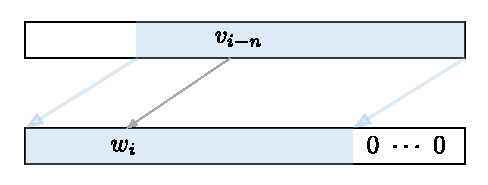
\includegraphics{figs/lsl}} &
\scalebox{.8}{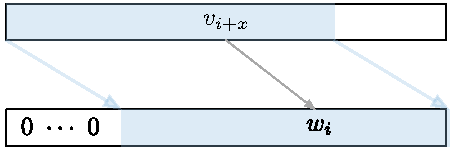
\includegraphics{figs/lsr}} \\
(a) Logical shift left: \holtxt{w = v << x}. & (b) Logical shift right:
\holtxt{w = v >>> x}. \\[12pt]
\scalebox{.8}{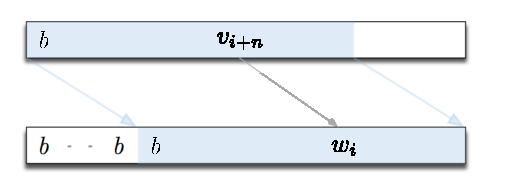
\includegraphics{figs/asr}} &
\hspace{-5mm}\scalebox{.8}{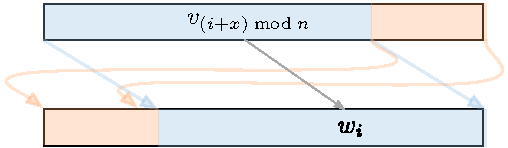
\includegraphics{figs/ror}} \\
(c) Arithmetic shift right: \holtxt{w = v >> x}. & (d) Rotate right: \holtxt{w
= v \#>> x}. \\[12pt]
\multicolumn{2}{c}{\scalebox{.8}{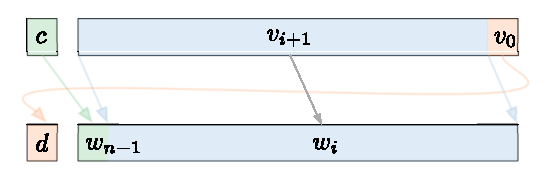
\includegraphics{figs/rrx}}} \\
\multicolumn{2}{c}{(e) Rotate right extended by 1 place: \holtxt{(d,w) =
word\_rrx (c,v)}.}
\end{tabular}
\caption{Shift operations.}
\label{fig:shifts}
\end{center}
\end{figure}

\paragraph{Arithmetic and orderings}

The arithmetic operations are: addition, subtraction, unary minus (two's
complement), logarithm (base-2), multiplication, modulus and division (signed and
unsigned).
These operations are defined with respect to the natural numbers.  For example,
word addition is defined by:
\begin{hol}
\begin{verbatim}
|- !v w. v + w = n2w (w2n v + w2n w)
\end{verbatim}
\end{hol}
The \holtxt{+} on the left-hand side is word addition and on the right it is
natural number addition.

All of the standard word orderings are provided, with signed and unsigned
versions of $<$, $\leq$, $>$ and $\geq$.  The unsigned versions are suffixed
with a plus; for example, \holtxt{<+} is unsigned ``less than''.

\paragraph{Constants}

The word theory also defines a few word constants:
\begin{center}\small
\begin{tabular}{lll}
\multicolumn{1}{l}{Constant} & \multicolumn{1}{l}{Value}  &
\multicolumn{1}{l}{Binary} \\
\noalign{\smallskip}
\hline
\noalign{\smallskip}
\holtxt{word\_T} or \holtxt{UINT\_MAXw} & $2^l - 1$ & $11\cdots 11$ \\
\holtxt{word\_L} or \holtxt{INT\_MINw} & $2^{l - 1}$ & $10\cdots 00$ \\
\holtxt{word\_H} or \holtxt{INT\_MAXw} & $2^{l - 1} - 1$ & $01\cdots 11$
\end{tabular}
\end{center}

\paragraph{List of bit vector operations}

A list of operations is provided in the table below.
{
\setlength{\tabcolsep}{4pt}
\begin{center}
\tablefirsthead{%
\hline
\multicolumn{1}{|c}{Operation\rule{0pt}{14pt}} &
\multicolumn{1}{c}{Symbol} &
Type &
\multicolumn{1}{c|}{Description} \\[4pt]
\hline}
\tablehead{%
\hline
\multicolumn{4}{|l|}{\small\sl continued from previous page}\\
\hline
\multicolumn{1}{|c}{Operation\rule{0pt}{14pt}} &
\multicolumn{1}{c}{Symbol} &
Type &
\multicolumn{1}{c|}{Description} \\[4pt]
\hline}
\tabletail{%
\hline
\multicolumn{4}{|r|}{\small\sl continued on next page}\\
\hline}
\tablelasttail{\hline}
\small
\begin{supertabular}{|l|c|l|l|}
\holtxt{n2w} & & \num\rarr\worda & Map from a natural number \\
\holtxt{w2n} & & \worda\rarr\num & Map to a natural number \\
\holtxt{w2w} & & \worda\rarr\wordb & Map word-to-word (unsigned) \\
\holtxt{sw2sw} & & \worda\rarr\wordb & Map word-to-word (signed) \\
\holtxt{w2l} & & \num\rarr\worda\rarr\num~\ty{list} & Map word to digit list \\
\holtxt{l2w} & & \num\rarr\num~\ty{list}\rarr\worda & Map digit list to word \\
\holtxt{w2s} & & \num\rarr(\num\rarr\ty{char})\rarr\worda\rarr\ty{string} & Map word to string \\
\holtxt{s2w} & & \num\rarr(\ty{char}\rarr\num)\rarr\ty{string}\rarr\worda & Map string to word \\
\holtxt{word\_len} & & \worda\rarr\num & The word length \\
\holtxt{word\_lsb} & & \worda\rarr\bool & The least significant bit \\
\holtxt{word\_msb} & & \worda\rarr\bool & The most significant bit \\
\holtxt{word\_bit} & & \num\rarr\worda\rarr\bool & Test bit position \\
\holtxt{word\_bits} & \holtxt{--} & \num\rarr\num\rarr\worda\rarr\worda & Select a bit field \\
\holtxt{word\_signed\_bits} & \holtxt{---} & \num\rarr\num\rarr\worda\rarr\worda & Sign-extend selected bit field \\
\holtxt{word\_slice} & \holtxt{''} & \num\rarr\num\rarr\worda\rarr\worda &  Set bits outside field to zero \\
\holtxt{word\_extract} & \holtxt{><} & \num\rarr\num\rarr\worda\rarr\wordb & Extract (cast) a bit field \\
\holtxt{word\_reverse} & & \worda\rarr\worda & Reverse the bit order \\
\holtxt{bit\_field\_insert} & & {\setlength{\tabcolsep}{0pt}\begin{tabular}[t]{ll}\num\rarr\num\rarr\worda\rarr\\\wordb\rarr\wordb\end{tabular}} & Insert a bit field \\
\holtxt{word\_modify} & & {\setlength{\tabcolsep}{0pt}\begin{tabular}[t]{ll}(\num\rarr\bool\rarr\bool)\rarr\\\worda\rarr\worda\end{tabular}} & Apply a function to each bit \\
\holtxt{word\_join} & & \worda\rarr\wordb\rarr\fcp{\bool}{$\alpha+\beta$} & Join words \\
\holtxt{word\_concat} & \holtxt{@@} & \worda\rarr\wordb\rarr\wordc & Concatenate words \\
\holtxt{concat\_word\_list} & & \worda~\ty{list}\rarr\wordb & Concatenate list of words \\
\holtxt{word\_replicate} & & \num\rarr\worda\rarr\wordb & Replicate word \\
\holtxt{word\_or} & \holtxt{||} & \worda\rarr\worda\rarr\worda & Bitwise disjunction \\
\holtxt{word\_xor} & \holtxt{??} & \worda\rarr\worda\rarr\worda & Bitwise exclusive-or \\
\holtxt{word\_and} & \holtxt{\&\&} & \worda\rarr\worda\rarr\worda & Bitwise conjunction \\
\holtxt{word\_nor} & \holtxt{\~{}||} & \worda\rarr\worda\rarr\worda & Bitwise NOR \\
\holtxt{word\_xnor} & \holtxt{\~{}??} & \worda\rarr\worda\rarr\worda & Bitwise XNOR \\
\holtxt{word\_nand} & \holtxt{\~{}\&\&} & \worda\rarr\worda\rarr\worda & Bitwise NAND \\
\holtxt{word\_reduce} & & {\setlength{\tabcolsep}{0pt}\begin{tabular}[t]{ll}(\bool\rarr\bool\rarr\bool)\rarr\\\worda\rarr\fcp{\bool}{1}\end{tabular}} & Word reduction \\
\holtxt{reduce\_or} & & \worda\rarr\fcp{\bool}{1} & Disjunction reduction \\
\holtxt{reduce\_xor} & & \worda\rarr\fcp{\bool}{1} & Exclusive-or reduction \\
\holtxt{reduce\_and} & & \worda\rarr\fcp{\bool}{1} & Conjunction reduction \\
\holtxt{reduce\_nor} & & \worda\rarr\fcp{\bool}{1} & NOR reduction \\
\holtxt{reduce\_xnor} & & \worda\rarr\fcp{\bool}{1} & XNOR reduction \\
\holtxt{reduce\_nand} & & \worda\rarr\fcp{\bool}{1} & NAND reduction \\
\holtxt{word\_{}1comp} & \holtxt{\~} & \worda\rarr\worda & One's complement \\
\holtxt{word\_{}2comp} & \holtxt{-} & \worda\rarr\worda & Two's complement \\
\holtxt{word\_add} & \holtxt{+} & \worda\rarr\worda\rarr\worda & Addition \\
\holtxt{word\_sub} & \holtxt{-} & \worda\rarr\worda\rarr\worda & Subtraction \\
\holtxt{word\_mul} & \holtxt{*} & \worda\rarr\worda\rarr\worda & Multiplication \\
\holtxt{word\_div} & \holtxt{//} & \worda\rarr\worda\rarr\worda & Division (unsigned) \\
\holtxt{word\_sdiv} & \holtxt{/} & \worda\rarr\worda\rarr\worda & Division (signed) \\
\holtxt{word\_mod} & & \worda\rarr\worda\rarr\worda & Modulus \\
\holtxt{word\_log2} & & \worda\rarr\worda & Logarithm base-2 \\
\holtxt{word\_lsl} & \holtxt{<<} & \worda\rarr\num\rarr\worda & Logical shift left \\
\holtxt{word\_lsr} & \holtxt{>>>} & \worda\rarr\num\rarr\worda & Logical shift right \\
\holtxt{word\_asr} & \holtxt{>>} & \worda\rarr\num\rarr\worda & Arithmetic shift right \\
\holtxt{word\_ror} & \holtxt{\#>>} & \worda\rarr\num\rarr\worda & Rotate right \\
\holtxt{word\_rol} & \holtxt{\#<<} & \worda\rarr\num\rarr\worda & Rotate left \\
\holtxt{word\_rrx} & & \bool\#\worda\rarr\bool\#\worda & Rotate right extended by 1 place \\
\holtxt{word\_lt} & \holtxt{<} & \worda\rarr\worda\rarr\bool & Signed ``less than'' \\
\holtxt{word\_le} & \holtxt{<=} & \worda\rarr\worda\rarr\bool & Signed ``less than or equal'' \\
\holtxt{word\_gt} & \holtxt{>} & \worda\rarr\worda\rarr\bool & Signed ``greater than'' \\
\holtxt{word\_ge} & \holtxt{>=} & \worda\rarr\worda\rarr\bool & Signed ``greater than or equal'' \\
\holtxt{word\_lo} & \holtxt{<+} & \worda\rarr\worda\rarr\bool & Unsigned ``less than''  \\
\holtxt{word\_ls} & \holtxt{<=+} & \worda\rarr\worda\rarr\bool & Unsigned ``less than or equal'' \\
\holtxt{word\_hi} & \holtxt{>+} & \worda\rarr\worda\rarr\bool & Unsigned ``greater than'' \\
\holtxt{word\_hs} & \holtxt{>=+} & \worda\rarr\worda\rarr\bool & Unsigned ``greater than or equal'' \\
\end{supertabular}
\end{center}}

\index{bit vectors, the HOL theory of@bit vectors, the \HOL{} theory of|)}
} % matches bracket at beginning of n-bit section, where some n-bit
  % specific macros are defined

\section{Sequences}

\HOL{} provides theories for various kinds of sequences: finite lists, lazy lists,
paths, and finite strings.

\subsection{Lists}\label{sec:list}
\index{list, the type operator in HOL logic@\ml{list}, the type operator in \HOL{} logic}
\index{types, in HOL logic@types, in \HOL{} logic!tools for construction of}
\index{lists, the HOL theory of@lists, the \HOL{} theory of|(}
\index{ lists, the HOL theory of@\ml{[} $\cdots$ \ml{;} $\cdots$ \ml{]} (lists, the \HOL{} theory of)|(}

\HOL{} lists are inductively defined finite sequences where each
element in a list has the same type. The theory \ml{list} introduces
the unary type operator $\alpha \; \konst{list}$ by a type definition
and a standard collection of list processing functions are
defined. The primitive constructors {\small\verb+NIL+} and {\small\verb+CONS+}
%
\begin{hol}
\index{NIL, the HOL constant@\holtxt{NIL}, the \HOL{} constant}
\index{CONS, the HOL constant@\holtxt{CONS}, the \HOL{} constant}
\begin{verbatim}
   NIL  : 'a list
   CONS : 'a -> 'a list -> 'a list
\end{verbatim}
\end{hol}
%
are used to build lists and have been defined from the representing type for
lists. The \HOL{} parser
%
\index{parsing, of HOL logic@parsing, of \HOL{} logic!of list expressions}
%
has been specially modified to parse the expression \holtxt{[]} into
\holtxt{NIL}, to parse the expression \holtxt{h::t} into \holtxt{CONS
  h t}, and to parse the expression \holtxt{[$t_1$;$t_2$;\dots;$t_n$]}
into \holtxt{CONS $t_1$ (CONS $t_2$ $\cdots$ (CONS $t_n$ NIL)
  $\cdots$)}.  The \HOL{} printer
%
\index{printing, in HOL logic@printing, in \HOL{} logic!of list expressions}
%
reverses these transformations.

\index{list theorems, in HOL logic@list theorems, in \HOL{} logic}
Based on the inductive characterization of the type, the following
fundamental theorems about lists are proved and stored in the theory
\ml{list}.

\begin{hol}
\index{list_Axiom@\ml{list\_Axiom}}
\index{axioms!non-primitive, of HOL logic@non-primitive, of \HOL{} logic!for lists}
\index{induction theorems, in HOL logic@induction theorems, in \HOL{} logic!for lists}
\index{characterizing theorem!for lists}
\begin{verbatim}
   list_Axiom
     |- !x f. ?fn. (fn [] = x) /\ (!h t. fn (h::t) = f(fn t)h t)
   list_INDUCT
     |- !P. P [] /\ (!t. P t ==> (!h. P(h::t))) ==> (!l. P l)
   list_CASES
     |- !l. (l = []) \/ (?t h. l = h::t)
   CONS_11
     |- !h t h' t'. (h::t = h'::t') = (h = h') /\ (t = t')
   NOT_NIL_CONS
     |- !h t. ~([] = h::t)
   NOT_CONS_NIL
     |- !h t. ~(h::t = [])
\end{verbatim}
\end{hol}

The theorem \ml{list\_Axiom} shown above is analogous to the primitive
recursion theorem
%
\index{primitive recursion theorem!for lists}
%
on the natural numbers discussed above in Section~\ref{num-prim-rec}.
It states the validity of primitive recursive definitions on lists,
and can be used to justify any such definition.  The \ML{} function
\ml{new\_recursive\_definition} uses this theorem to do
automatic
%
\index{primitive recursion theorem!automated use of, in HOL system@automated use of, in \HOL{} system|)}
%
proofs of the existence of primitive recursive functions on lists and
then make constant specifications to introduce constants that denote
such functions.

The induction theorem for lists, \ml{list\_INDUCT}, provides the main
proof tool used to reason about operations that manipulate lists. The
theorem \ml{list\_CASES} is used to perform case analysis on whether a
list is empty or not.

The theorem {\small\verb+CONS_11+} shows that {\small\verb+CONS+} is injective;
the theorems {\small\verb+NOT_NIL_CONS+} and {\small\verb+NOT_CONS_NIL+} show that
{\small\verb+NIL+} and {\small\verb+CONS+} are distinct, \ie,
cannot give rise to the same structure. Together, these three theorems
are used for equational reasoning about lists.

The predicate \ml{NULL} and the selectors
%
\index{selectors, in HOL logic@selectors, in \HOL{} logic!for lists}
%
\ml{HD} and \ml{TL} are defined in the theory \theoryimp{list} by
%
\begin{hol}
\index{NULL, the HOL constant@\ml{NULL}, the \HOL{} constant}
\index{HD, the HOL constant@\ml{HD}, the \HOL{} constant}
\index{TL, the HOL constant@\ml{TL}, the \HOL{} constant}
\begin{verbatim}
   NULL |- NULL [] /\ (!h t. ~NULL(h::t))
   HD   |- !h t. HD(h::t) = h
   TL   |- !h t. TL(h::t) = t
\end{verbatim}
\end{hol}

\noindent The following functions on lists are also defined in the theory \ml{list}.
%
%
\paragraph{Case expressions}
\index{case expressions!over lists}

Compound \HOL{} expressions that branch based on whether a term is an
empty or non-empty list have the surface syntax (roughly borrowed from
ML)
\begin{hol}
\begin{verbatim}
   case e1
    of [] => e2
     | (h::t) => e3
\end{verbatim}
\end{hol}
%
Such an expression is translated to
$\holtxt{list\_CASE}\ e_1\ e_2\ (\lambda h\; t.\ e_3)$ where the constant
\holtxt{list\_CASE} is defined as follows:
\begin{hol}
\begin{verbatim}
   list_case_def
     |- (!v f. list_CASE [] v f = v) /\
        (!v f a0 a1. list_CASE (a0::a1) v f = f a0 a1)
\end{verbatim}
\end{hol}

\paragraph{List membership}
\index{MEM, the HOL constant@\ml{MEM}, the \HOL{} constant}

Membership in a list, \ml{MEM}, is defined as follows:
%
\begin{hol}
\begin{verbatim}
   MEM |- (!x. MEM x [] = F) /\
          (!x h t. MEM x (h::t) = (x = h) \/ MEM x t)
\end{verbatim}
\end{hol}

\paragraph {Concatenation of lists}
\index{APPEND, the HOL constant@\ml{APPEND}, the \HOL{} constant}
\index{concatenation, of lists!in HOL logic@in \HOL{} logic}
\index{FLAT, the HOL constant@\ml{FLAT}, the \HOL{} constant}

Binary list concatenation ({\small\verb+APPEND+}) may also be denoted by
the infix operator {\small\verb|++|}; thus the expression
{\small\verb|L1 ++ L2|} is translated into {\small\verb+APPEND L1 L2+}.
The concatenation of a list of lists into a list is achieved by
{\small\verb+FLAT+}.
%
\begin{hol}
\begin{verbatim}
   APPEND
     |- (!l. APPEND [] l = l) /\
        (!l1 l2 h. APPEND (h::l1) l2 = h::APPEND l1 l2)
   FLAT
     |- (FLAT [] = []) /\ (!h t. FLAT(h::t) = h ++ FLAT t)
\end{verbatim}
\end{hol}

\paragraph {Numbers and lists}
\index{LENGTH, the HOL constant@\ml{LENGTH}, the \HOL{} constant}
\index{EL, the HOL constant@\ml{EL}, the \HOL{} constant}
\index{list_size, the HOL constant@\ml{list\_size}, the \HOL{} constant}

The length (\holtxt{LENGTH}) and size (\holtxt{list\_size}) of a list
are related notions. The size of a list takes account of the size of
each element of the list (given by parameter
$f:\alpha\to\konst{num}$), while the length of the list ignores the
size of each list element. The alternate length definition
(\holtxt{LEN}) is tail-recursive.  Numbers can also be used to index
into lists, extracting the element at the specified position.
%
\begin{hol}
\begin{verbatim}
   LENGTH
     |- (LENGTH [] = 0) /\ (!h t. LENGTH (h::t) = SUC(LENGTH t))
   LEN_DEF
     |- (!n. LEN [] n = n) /\ !h t n. LEN (h::t) n = LEN t (n + 1)
   list_size_def
     |- (!f. list_size f [] = 0) /\
        !f a0 a1. list_size f (a0::a1) = 1 + (f a0 + list_size f a1))
   EL
     |- (!l. EL 0 l = HD l) /\ (!l n. EL (SUC n) l = EL n (TL l))
\end{verbatim}
\end{hol}

\noindent
Note that the extraction of the $n$th element (\holtxt{EL}) of a list
starts its indexing from 0.  If the length of the list $\ell$ is less
than or equal to $n$, the result of \holtxt{EL~$n$~$\ell$~} is
unspecified.

\paragraph {Mapping functions over lists}
\index{MAP, the HOL constant@\ml{MAP}, the \HOL{} constant}
\index{MAP2, the HOL constant@\ml{MAP2}, the \HOL{} constant}
\index{mapping functions, in the HOL logic@mapping functions, in the \HOL{} logic!for lists}

There are functions for mapping a function $f : \alpha \to \beta$ over
a single list (\holtxt{MAP}) or a function $f : \alpha \to \beta
\to \gamma$ over two lists (\holtxt{MAP2}).
\begin{hol}
\begin{verbatim}
   MAP
     |- (!f. MAP f [] = []) /\
        (!f h t. MAP f (h::t) = f h::MAP f t)
   MAP2
     |- (!f. MAP2 f [] [] = []) /\
        !f h1 t1 h2 t2. MAP2 f (h1::t1) (h2::t2) = f h1 h2::MAP2 f t1 t2
\end{verbatim}
\end{hol}
The behaviour of \holtxt{MAP2} in the cases when it is given lists of
unequal lengths is unspecified.

\paragraph {Predicates over lists}
\index{FILTER, the HOL constant@\ml{FILTER}, the \HOL{} constant}
\index{EVERY, the HOL constant@\ml{EVERY}, the \HOL{} constant}
\index{ALL_DISTINCT, the HOL constant@\ml{ALL\_DISTINCT}, the \HOL{} constant}
\index{EXISTS, the HOL constant (over lists)@\ml{EXISTS}, the \HOL{}
  constant (over lists)}

Predicates can be applied to lists in a universal sense (the predicate
must hold of every element in the list) or an existential sense (the
predicate must hold of some element in the list). This functionality
is supported by \holtxt{EVERY} and \holtxt{EXISTS}, respectively. The
elimination of all elements in list not satisfying a given predicate
is performed by \holtxt{FILTER}.
\begin{hol}
\begin{verbatim}
   EVERY_DEF
     |- (!P. EVERY P [] = T) /\
        (!P h t. EVERY P (h::t) = P h /\ EVERY P t)
   EXISTS_DEF
     |- (!P. EXISTS P [] = F) /\
        (!P h t. EXISTS P (h::t) = P h \/ EXISTS P t)
   FILTER
     |- (!P. FILTER P [] = []) /\
        (!P h t. FILTER P (h::t) = if P h then h::FILTER P t else FILTER P t)
   ALL_DISTINCT
     |- (ALL_DISTINCT [] = T) /\
        (!h t. ALL_DISTINCT (h::t) = ~MEM h t /\ ALL_DISTINCT t)
\end{verbatim}
\end{hol}
The predicate \holtxt{ALL\_DISTINCT} holds on a list just in case no
element in the list is equal to any other.

\paragraph {Folding}
\index{FOLDL, the HOL constant@\ml{FOLDL}, the \HOL{} constant}
\index{FOLDR, the HOL constant@\ml{FOLDR}, the \HOL{} constant}

Applying a binary function $f : \alpha\to\beta\to\beta$ pairwise
through a list and accumulating the result is known as
\emph{folding}. At times, it is necessary to do this operation
from left-to-right (\holtxt{FOLDL}), and at others the
right-to-left direction (\holtxt{FOLDR}) is required.
\begin{hol}
\begin{verbatim}
   FOLDL
     |- (!f e. FOLDL f e [] = e) /\
        (!f e x l. FOLDL f e (x::l) = FOLDL f (f e x) l)
   FOLDR
     |- (!f e. FOLDR f e [] = e) /\
        (!f e x l. FOLDR f e (x::l) = f x (FOLDR f e l))
\end{verbatim}
\end{hol}

\paragraph {List reversal}

The reversal of a list (\holtxt{REVERSE}) and its tail recursive
counterpart \holtxt{REV} are defined in \theoryimp{list}.
\begin{hol}
\begin{verbatim}
   REVERSE_DEF
     |- (REVERSE [] = []) /\
        (!h t. REVERSE (h::t) = REVERSE t ++ [h])
   REV_DEF
     |- (!acc. REV [] acc = acc) /\
        (!h t acc. REV (h::t) acc = REV t (h::acc))
\end{verbatim}
\end{hol}

\paragraph {Removal of duplicates}
The \holtxt{nub} function removes all duplicate entries from a list.
\begin{hol}
\begin{verbatim}
   nub_DEF
     |- (nub [] = []) /\
        (!x l. nub (x::l) = if MEM x l then nub l else x::nub l)
\end{verbatim}
\end{hol}

\paragraph {Conversion to sets}

Lists can be converted to sets (\ml{LIST\_TO\_SET}) by partial
application of \holtxt{MEM}. The somewhat terse definition is used to
derive the theorem \ml{IN\_LIST\_TO\_SET}.
%
\begin{hol}
\begin{verbatim}
  LIST_TO_SET
    |- LIST_TO_SET = combin$C MEM
  IN_LIST_TO_SET
    |- x IN LIST_TO_SET l = MEM x l
\end{verbatim}
\end{hol}
%
Further support for translating between different kinds of
collections may be found in the \theoryimp{container} theory.

\paragraph {Pairs and lists}

Two lists of equal length may be component-wise paired by
the {\small\verb+ZIP+} operation. The result is unspecified
when the lists are not the same length. The inverse operation,
{\small\verb+UNZIP+}, translates a list of pairs into a pair of
lists.
\begin{hol}
\begin{verbatim}
  ZIP
    |- (ZIP ([],[]) = []) /\
       (!x1 l1 x2 l2. ZIP (x1::l1,x2::l2) = (x1,x2)::ZIP (l1,l2))
  UNZIP_THM
    |- (UNZIP [] = ([],[])) /\
       (UNZIP ((x,y)::t) = let (L1,L2) = UNZIP t in (x::L1,y::L2))
\end{verbatim}
\end{hol}

\paragraph {Alternate access}
\index{LAST, the HOL constant@\ml{LAST}, the \HOL{} constant}
\index{FRONT, the HOL constant@\ml{FRONT}, the \HOL{} constant}
%
Lists are essentially treated in a stack-like manner. However, at
times it is convenient to access the last element
(\holtxt{LAST}) of a non-empty list directly. The last element
of a non-empty list is dropped by \holtxt{FRONT}.
\begin{hol}
\begin{verbatim}
  LAST_DEF
    |- !h t. LAST (h::t) = if t = [] then h else LAST t
  FRONT_DEF
    |- !h t. FRONT (h::t) = if t = [] then [] else h::FRONT t
  APPEND_FRONT_LAST
    |- !l. ~(l = []) ==> (FRONT l ++ [LAST l] = l)
\end{verbatim}
\end{hol}
%
Joining the front part and the last element of a non-empty list yields
the original list.  Both \holtxt{LAST} and \holtxt{FRONT}
are unspecified on empty lists.


\paragraph {Prefix checking}

\index{isPREFIX, the HOL constant@\ml{isPREFIX}, the \HOL{} constant}
The relation capturing whether a list $\ell_1$ is a prefix of $\ell_2$
({\holtxt{isPREFIX}) can be defined by recursion. The infix
\holtxt{<{}<=} can also be used as notation for this partial order.
% use of {} above is just a trick to stop Emacs font-lock colouring
% this file disgustingly
%
\begin{hol}
\begin{verbatim}
   isPREFIX_THM
     |- ([] <<= l <=> T) /\
        (h::t <<= [] <=> F) /\
        (h1::t1 <<= h2::t2 <=> (h1 = h2) /\ t1 <<= t2)
\end{verbatim}
\end{hol}
The above theorem states that: the empty list is a prefix of any other
list (clause 1); that no non-empty list is a prefix of the empty list
(clause 2); and that a non-empty list is a prefix of another non-empty
list if the first elements of the lists are the same, and if the tail
of the first is a prefix of the tail of the second.

\vspace{1ex}
\noindent For a complete list of available theorems in
\theoryimp{list}, see \REFERENCE.  Further development of list
theory can be found in \theoryimp{rich\_list}.


\subsubsection{List permutations and sorting}
\index{permutations (of lists), the HOL theory of@permutations (of lists), the \HOL{} theory of}
\index{sorting, the HOL theory of@sorting, the \HOL{} theory of}

The \theoryimp{sorting} theory defines a notion of two lists being
permutations of each other, then defines a general notion of sorting,
then shows that Quicksort is a sorting function. The 
\theoryimp{mergesort} theory defines Merge sort and shows that it is a stable
sorting function.

\paragraph{List permutation}

Two lists are in permutation if they have exactly the same members,
and each member has the same number of occurrences in both lists. One
definition (\holtxt{PERM}) that captures this relationship is the
following:
%
\begin{hol}
\begin{verbatim}
   PERM_DEF
     |- !L1 L2. PERM L1 L2 = !x. FILTER ($= x) L1 = FILTER ($= x) L2
   PERM_IND =
     |- !P.
          P [] [] /\
          (!x l1 l2. P l1 l2 ==> P (x::l1) (x::l2)) /\
          (!x y l1 l2. P l1 l2 ==> P (x::y::l1) (y::x::l2)) /\
          (!l1 l2 l3. P l1 l2 /\ P l2 l3 ==> P l1 l3)
         ==>
         !l1 l2. PERM l1 l2 ==> P l1 l2
\end{verbatim}
\end{hol}
%
A derived induction theorem (\holtxt{PERM\_IND}) is very
useful in proofs about permutations.

\paragraph{Sorting}

A list is $R$-sorted if $R$ holds pairwise through the list. This
notion (\holtxt{SORTED}) is captured by a recursive definition. Then
a function of type
%
\begin{hol}
\begin{verbatim}
   ('a -> 'a -> bool) -> 'a list -> 'a list
\end{verbatim}
\end{hol}
%
is a sorting function (\holtxt{SORTS}) with respect to $R$ if
it delivers a permutation of its input, and the result is $R$-sorted.
%
\begin{hol}
\begin{verbatim}
   SORTED_DEF
     |- (SORTED R [] = T) /\
        (SORTED R [x] = T) /\
        (SORTED R (x::y::rst) = R x y /\ SORTED R (y::rst))
   SORTS_DEF
     |- !f R. SORTS f R = !l. PERM l (f R l) /\ SORTED R (f R l)
\end{verbatim}
\end{hol}
%
Quicksort is defined in the usual functional programming style, and
it is indeed a sorting function, provided $R$ is a transitive and
total relation.
%
\begin{hol}
\begin{verbatim}
   QSORT_DEF =
     |- (QSORT ord [] = []) /\
        (QSORT ord (h::t) =
           let (l1,l2) = PARTITION (\y. ord y h) t
           in
             QSORT ord l1 ++ [h] ++ QSORT ord l2)
   QSORT_SORTS
     |- !R. transitive R /\ total R ==> SORTS QSORT R
\end{verbatim}
\end{hol}



\index{lists, the HOL theory of@lists, the \HOL{} theory of|)}
\index{ lists, the HOL theory of@\ml{[} $\cdots$ \ml{;} $\cdots$ \ml{]} (lists, the \HOL{} theory of)|)}

\subsection{Possibly infinite sequences (\theoryimp{llist})}

\index{lazy lists, the HOL theory of@``lazy'' lists, the \HOL{} theory of|(}

The theory \theoryimp{llist} contains the definition of a type of
possibly infinite sequences.  This type is similar to the ``lazy
lists'' of programming languages like Haskell, hence the name of the
theory.  The \theoryimp{llist} theory has a number of constants that
are analogous to constants in the theory of finite
lists.  The \theoryimp{llist} versions of these constants have the
same names, but with a capital `L\/' prepended.  Thus, some of the core
constants in this theory are:
\begin{hol}
\begin{verbatim}
   LNIL  : 'a llist
   LCONS : 'a -> 'a llist -> 'a llist
   LHD   : 'a llist -> 'a option
   LTL   : 'a llist -> 'a llist option
\end{verbatim}
\end{hol}

The \ml{LHD} and \ml{LTL} constants return \ml{NONE} when applied to
the empty sequence, \ml{LNIL}.  This use of an option type is another
way of modelling the essential partiality of these constants.  (In the
theory of lists, the analogous \ml{HD} and \ml{TL} functions simply
have unspecified values when applied to empty lists.)

The type \ml{llist} is not inductive, and there is no primitive
recursion theorem supporting the definition of functions that have
domains of type \ml{llist}.  Rather, \ml{llist} is a coinductive type,
and has an axiom that justifies the definition of (co-)recursive
functions that map \emph{into} the \ml{llist} type:
\begin{hol}
\begin{verbatim}
   llist_Axiom
      |- !f : 'a -> ('a # 'b) option.
           ?g : 'a -> 'b llist.
             (!x. LHD (g x) = OPTION_MAP SND (f x)) /\
             (!x. LTL (g x) = OPTION_MAP (g o FST) (f x))
\end{verbatim}
\end{hol}
\noindent An equivalent form of the above is
\begin{hol}
\begin{verbatim}
   llist_Axiom_1
      |- !f. ?g.
           !x. g x =
               case f x
                of NONE => LNIL
                 | SOME (x',y) => LCONS y (g x')
\end{verbatim}
\end{hol}

Other constants in the theory \theoryimp{llist} include \ml{LMAP}, \ml{LFINITE},
\ml{LNTH}, \ml{LTAKE}, \ml{LDROP}, and \ml{LFILTER}. Their types are
%
\index{mapping functions, in the HOL logic@mapping functions, in the \HOL{} logic!for possibly infinite sequences}
\begin{hol}
\begin{verbatim}
   LMAP    : ('a -> 'b) -> 'a llist -> 'b llist
   LFINITE : 'a llist -> bool
   LNTH    : num -> 'a llist -> 'a option
   LTAKE   : num -> 'a llist -> 'a list option
   LDROP   : num -> 'a llist -> 'a llist option
   LFILTER : ('a -> bool) -> 'a llist -> 'a llist
\end{verbatim}
\end{hol}
They are characterised by the following theorems
\begin{hol}
\begin{verbatim}
   LMAP
      |- (LMAP f LNIL = LNIL) /\
         (LMAP f (LCONS h t) = LCONS (f h) (LMAP f t))
   LFINITE_THM
      |- (LFINITE LNIL = T) /\
         (LFINITE (LCONS h t) = LFINITE t)
   LNTH_THM
      |- (!n. LNTH n LNIL = NONE) /\
         (!h t. LNTH 0 (LCONS h t) = SOME h) /\
         (!n h t. LNTH (SUC n) (LCONS h t) = LNTH n t)
   LTAKE_THM
      |- (LTAKE 0 l = SOME []) /\
         (LTAKE (SUC n) LNIL = NONE) /\
         (LTAKE (SUC n) (LCONS h t) = OPTION_MAP (CONS h) (LTAKE n t)
   LDROP_THM
      |- (LDROP 0 ll = SOME ll) /\
         (LDROP (SUC n) ll = NONE) /\
         (LDROP (SUC n) (LCONS h t) = LDROP n t)
   LFILTER_THM
      |- (LFILTER P LNIL = LNIL) /\
         (LFILTER P (LCONS h t) = if P h then LCONS h (LFILTER P t)
                                         else LFILTER P t)
\end{verbatim}
\end{hol}

\paragraph{Concatenation}

Two lazy lists may be concatenated by \ml{LAPPEND}. If the first lazy
list is infinite, elements of the second are inaccessible in the
result.  A lazy list of lazy lists can be flattened to a lazy list by
\ml{LFLATTEN}.
\begin{hol}\begin{verbatim}
   LAPPEND
      |- (!x. LAPPEND LNIL x = x) /\
         (!h t x. LAPPEND (LCONS h t) x = LCONS h (LAPPEND t x))
   LFLATTEN_THM
      |- (LFLATTEN LNIL = LNIL) /\
         (!tl. LFLATTEN (LCONS LNIL t) = LFLATTEN t) /\
         (!h t tl. LFLATTEN (LCONS (LCONS h t) tl) =
                      LCONS h (LFLATTEN (LCONS t tl)))
\end{verbatim}\end{hol}

\paragraph{Lists and lazy lists}

Mapping back and forth from lists to lazy lists is accomplished
by \ml{fromList} and \ml{toList}:
\begin{hol}\begin{verbatim}
   fromList
      |- (fromList [] = LNIL) /\
         (!h t. fromList (h::t) = LCONS h (fromList t))
   toList_THM
      |- (toList LNIL = SOME []) /\
         (!h t. toList (LCONS h t) = OPTION_MAP (CONS h) (toList t))
\end{verbatim}\end{hol}

\paragraph{Proof principles}

Finally, there are two very important proof principles for proving
that two \ml{llist} values are equal.  The first states that two
sequences are equal if they return the same prefixes of length $n$ for
all possible values of $n$:
\begin{hol}
\begin{verbatim}
   LTAKE_EQ |- (ll1 = ll2) = (!n. LTAKE n ll1 = LTAKE n ll2)
\end{verbatim}
\end{hol}
This theorem is subsequently used to derive the bisimulation
principle:
\begin{hol}
\begin{verbatim}
   LLIST_BISIMULATION
            |- (ll1 = ll2) =
               ?R. R ll1 ll2 /\
                   !ll3 ll4. R ll3 ll4 ==>
                             (ll3 = LNIL) /\ (ll4 = LNIL) \/
                             (LHD ll3 = LHD ll4) /\
                             R (THE (LTL ll3)) (THE (LTL ll4))
\end{verbatim}
\end{hol}
The principle of bisimulation states that two \ml{llist} values $l_1$
and $l_2$ are equal if (and only if) it is possible to find a
relation $R$ such that
\begin{itemize}
\item $R$ relates the two values, i.e., $R\;l_1\;l_2$; and
\item if $R$ holds of any two values $l_3$ and $l_4$, then either
  \begin{itemize}
  \item both $l_3$ and $l_4$ are empty; or
  \item the head elements of $l_3$ and $l_4$ are the same, and the
    tails of those two values are again related by $R$
  \end{itemize}
\end{itemize}
Of course, a possible $R$ would be equality itself, but the strength
of this theorem is that other, more convenient relations can also be
used.
\index{lazy lists, the HOL theory of@``lazy'' lists, the \HOL{} theory of|)}

\subsection{Labelled paths (\theoryimp{path})}

The theory \theoryimp{path}
%
\index{labelled paths, the HOL theory of@labelled paths, the \HOL{} theory of|(}%
\index{reduction sequences, the HOL theory of@reduction sequences, the \HOL{} theory of|(}%
\index{paths (reduction sequences), the HOL theory of@paths (reduction sequences), the \HOL{} theory of|(}%
%
defines a binary type operator $(\alpha,\beta)\ml{path}$, which
stands for possibly infinite paths of the following form
\[
  \alpha_1 \stackrel{\beta_1}{\longrightarrow}
  \alpha_2 \stackrel{\beta_2}{\longrightarrow}
  \alpha_3 \stackrel{\beta_3}{\longrightarrow} \cdots
  \alpha_n \stackrel{\beta_n}{\longrightarrow}
  \alpha_{n+1} \stackrel{\beta_{n+1}}{\longrightarrow}  \cdots
  \]
The \ml{path} type is thus an appropriate model for reduction
sequences, where the $\alpha$ parameter corresponds to ``states'', and
the $\beta$ parameter corresponds to the labels on the arrows.

The model of $(\alpha,\beta)\ml{path}$ is $\alpha \times
((\alpha\times\beta)\ml{llist})$.  The type of paths has two
constructors:
\begin{hol}
\begin{verbatim}
   stopped_at : 'a -> ('a,'b) path
   pcons      : 'a -> 'b -> ('a,'b) path -> ('a,'b) path
\end{verbatim}
\end{hol}
The \holtxt{stopped\_at} constructor returns a path containing just one
state, and no transitions.  (Thus, the reduction sequence has
``stopped at'' this state.)  The \ml{pcons} constructor takes a state,
a label, and a path, and returns a path which is now headed by the
state argument, and which moves from that state via the label argument
to the path.  Graphically, $\ml{pcons}\;x\;l\;p$ is equal to
\[
x \stackrel{l}{\longrightarrow}
\underbrace{p_1 \stackrel{l_1}{\longrightarrow} p_2
  \stackrel{l_2}{\longrightarrow} \cdots\quad}_p
\]
Other constants defined in theory \theoryimp{path} include
%
\index{mapping functions, in the HOL logic@mapping functions, in the \HOL{} logic!for labelled paths}
%
\begin{hol}
\begin{verbatim}
   finite  : ('a,'b) path -> bool
   first   : ('a,'b) path -> 'a
   labels  : ('a,'b) path -> 'b llist
   last    : ('a,'b) path -> 'a
   length  : ('a,'b) path -> num option
   okpath  : ('a -> 'b -> 'a -> bool) -> ('a,'b) path -> bool
   pconcat : ('a,'b) path -> 'b -> ('a,'b) path -> ('a,'b) path
   pmap    : ('a -> 'c) -> ('b -> 'd) -> ('a,'b)path -> ('c,'d)path
\end{verbatim}
\end{hol}

The \ml{first} function returns the first element of a path.
There always is such an element, and the defining equations are
\begin{hol}
\begin{verbatim}
   first_thm  |- (first (stopped_at x) = x) /\
                 (first (pcons x l p) = x)
\end{verbatim}
\end{hol}

On the other hand, the \ml{last} function does not always have a
well-specified value, though it still has nice characterising
equations:
\begin{hol}
\begin{verbatim}
   last_thm   |- (last (stopped_at x) = x) /\
                 (last (pcons x l p) = last p)
\end{verbatim}
\end{hol}

The theorem for \ml{finite} has a similar feel, but has a definite
value (\ml{F}, or \emph{false}) on infinite paths), whereas the
value of \ml{last} on such paths is unspecified:
\begin{hol}
\begin{verbatim}
   finite_thm |- (finite (stopped_at x) = T) /\
                 (finite (pcons x l p) = finite p)
\end{verbatim}
\end{hol}

The function \ml{pconcat} concatenates two paths, linking them
with a provided label.  If the first path is infinite, then the result
is equal to that first path.  The defining equation is
\begin{hol}
\begin{verbatim}
   pconcat_thm |- (pconcat (stopped_at x) lab p2 = pcons x lab p2) /\
                  (pconcat (pcons x r p) lab p2 =
                       pcons x r (pconcat p lab p2)
\end{verbatim}
\end{hol}
%
These equations are true even when the first argument to
\ml{pconcat} is an infinite path.

The \ml{okpath} predicate tests whether or not a path is a valid
transition given a ternary transition relation.  Its characterising
theorem is
\begin{hol}
\begin{verbatim}
  okpath_thm |-
     (okpath R (stopped_at x)) /\
     (okpath R (pcons x r p) = R x r (first p) /\ okpath R p)
\end{verbatim}
\end{hol}
%
There is also an induction principle that simplifies reasoning about
finite $R$-paths:
%
\begin{hol}
\begin{verbatim}
   finite_okpath_ind |-
       (!x. P (stopped_at x)) /\
       (!x r p. okpath R p /\ finite p /\ R x r (first p) /\ P p ==>
                P (pcons x r p)) ==>
       !p. okpath R p /\ finite p ==> P p
\end{verbatim}
\end{hol}

One can show that a set \holtxt{P} of paths are all $R$-paths with the
co-induction principle:
\begin{hol}
\begin{verbatim}
   okpath_co_ind |-
      !P.
         (!x r p. P (pcons x r p) ==> R x r (first p) /\ P p) ==>
         !p. P p ==> okpath R p
\end{verbatim}
\end{hol}
\index{labelled paths, the HOL theory of@labelled paths, the \HOL{} theory of|)}
\index{reduction sequences, the HOL theory of@reduction sequences, the \HOL{} theory of|)}
\index{paths (reduction sequences), the HOL theory of@paths (reduction sequences), the \HOL{} theory of|)}


\subsection{Character strings (\theoryimp{string})}
\index{strings, the HOL theory of@strings, the \HOL{} theory of|(}

The theory \theoryimp{string} defines a type of characters and a type
of finite strings built from those characters, along with a useful suite of
definitions for operating on strings.

\paragraph {Characters}
\index{characters, the HOL theory of@characters, the \HOL{} theory of}

The type \holtxt{char} is represented by the numbers less than 256. Two
constants are defined: {\small\verb+CHR +}$: \konst{num}\to\konst{char}$ and
{\small\verb+ORD +}$: \konst{char}\to\konst{num}$. The following theorems
hold:
\begin{hol}
\begin{verbatim}
  CHR_ORD  |- !a. CHR (ORD a) = a
  ORD_CHR  |- !r. r < 256 = (ORD (CHR r) = r)
\end{verbatim}
\end{hol}

\index{character literals}
Character literals can also be entered using \ML{} syntax, with a hash
character immediately followed by a string literal of length one.
Thus:
\setcounter{sessioncount}{0}
\begin{session}
\begin{verbatim}
- val t = ``f #"c" #"\n"``;
<<HOL message: inventing new type variable names: 'a>>
> val t = ``f #"c" #"\n"`` : term

- dest_term ``#"\t"``;
> val it = COMB(``CHR``, ``9``) : lambda
\end{verbatim}
\end{session}



\paragraph {Strings}

The type \holtxt{string} is an alias for the type \holtxt{char list}.
All functions and predicates over lists are thus available for use
over strings.  Some of these constants are overloaded so that they are
printed (and can be parsed) with names that are more appropriate for
the particular case of lists of characters.

For example, \holtxt{NIL} and \holtxt{CONS} over strings have
alternative names \holtxt{EMPTYSTRING} and \holtxt{STRING}
respectively:
%
\begin{hol}
\index{EMPTYSTRING, the HOL constant@\holtxt{EMPTYSTRING}, the \HOL{} constant}
\index{STRING, the HOL constant@\holtxt{STRING}, the \HOL{} constant}
\begin{verbatim}
   EMPTYSTRING : string
   STRING      : char -> string -> string
\end{verbatim}
\end{hol}
\index{string literals}
The \HOL{} parser maps the syntax \holtxt{""} to \holtxt{EMPTYSTRING},
and the \HOL{} printer inverts this.  The parser expands string
literals of the form \holtxt{"$c_1 c_2 \ldots c_n$"} to the compound
term
\[
\holtxt{STRING} \;c_1\; (\holtxt{STRING}\;c_2\,\ldots\,
 (\holtxt{STRING} \;c_{n-1} \; (\holtxt{STRING}\;
c_n \; \holtxt{EMPTYSTRING})) \,\ldots\, )
\]
Of course, one could also write
\begin{session}
\begin{verbatim}
- ``[#"a"; #"b"]``;
> val it = ``"ab"`` : term
\end{verbatim}
\end{session}

String literals can be constructed using the various special escape
sequences that are used in \ML{}.  For example, \ml{\bs{}n} for the
newline character, and a backslash followed by three decimal digits
for characters of the given number.
\begin{session}
\begin{verbatim}
- val t = ``"foo bar\n\001"``;
> val t = ``"foo bar\n\^A"`` : term
\end{verbatim}
\end{session}
Note that if one wants to use the control-character syntax with the
caret that the pretty-printer has chosen to use in printing the given
string, and this occurs inside a quotation, then the caret will need
to be doubled.  (See Section~\ref{sec:quotation-antiquotation}.)

There is also a destructor function {\small\verb+DEST_STRING+} for
strings which returns an option type.
\begin{hol}
\begin{verbatim}
   DEST_STRING
     |- (DEST_STRING "" = NONE) /\
        (DEST_STRING (STRING c rst) = SOME(c,rst))
\end{verbatim}
\end{hol}


\paragraph{Case expressions}
\index{case expressions!over strings}

Compound \HOL{} expressions that branch based on
whether a term is an empty or non-empty string can be written with the
surface syntax
\begin{hol}
\begin{verbatim}
   case s
    of "" => e1
     | STRING c rst => e2
\end{verbatim}
\end{hol}

Such an expression is actually a case-expression over the underlying list, and so the underlying constant is that for lists.

\paragraph {Length and concatenation}

A standard function \holtxt{LENGTH} can be written \holtxt{STRLEN}
when applied to a string, and \holtxt{APPEND} can be written as
\holtxt{STRCAT}.  There are also theorems characterising these
constants in \ml{stringTheory}, though they are simply instantiations
of results from \ml{listTheory}:
\begin{hol}
\begin{verbatim}
   STRLEN_THM
     |- (STRLEN "" = 0) /\
        (STRLEN (STRING c s) = 1 + STRLEN s)

   STRCAT_EQNS =
     |- (STRCAT "" s = s) /\
        (STRCAT s "" = s) /\
        (STRCAT (STRING c s1) s2 = STRING c (STRCAT s1 s2))
\end{verbatim}
\end{hol}


\index{strings, the HOL theory of@strings, the \HOL{} theory of|)}

\section{Collections}

Several different notions of a collection of elements are available in
\HOL: sets, multisets, relations, and finite maps.

\subsection{Sets (\theoryimp{pred\_set})}
\label{sec:theory-of-sets}
\index{sets, the HOL theory of@sets, the \HOL{} theory of}

An extensive development of set theory is available in the theory
\theoryimp{pred\_set}. Sets are represented by functions of the type
$\alpha \to \konst{bool}$, \ie, they are so-called characteristic
functions.
%
\index{characteristic functions!as basis for \HOL{} theory of sets}
%
One can use the type abbreviation $\alpha\; \konst{set}$
instead of $\alpha \to \konst{bool}$. Sets may be finite or
infinite. All of the elements in a set must have the same type.

\emph{Set membership} is the basic notion that formalized set theory
is based on. In \HOL, membership is represented by a the infix
constant \holtxt{IN}, defined in theory \theoryimp{bool} for
convenience.
\begin{hol}
\begin{verbatim}
   IN_DEF   |- IN = \x f. f x
\end{verbatim}
\end{hol}
The \holtxt{IN} operator is merely a way of applying the
characteristic function to an item, as the following trivial
consequence of the definition shows:
\begin{hol}
\begin{verbatim}
   SPECIFICATION   |- !P x. x IN P = P x
\end{verbatim}
\end{hol}
Two sets are equal if they have the same elements.
\begin{hol}
\begin{verbatim}
   EXTENSION   |- !s t. (s = t) = (!x. (x IN s) = (x IN t))
\end{verbatim}
\end{hol}

\paragraph{Empty and universal sets}
\index{universal set}
The empty set is the characteristic function that is constantly false. The constant \holtxt{EMPTY} denotes the empty set; it may be written as \holtxt{\{\}} and \holtxt{$\emptyset$} (U+2205).
The universal set, \holtxt{UNIV}, on a type is the characteristic function that is always true for elements of that type.
\begin{hol}
\begin{verbatim}
   EMPTY_DEF   |- {} = (\x. F)
   UNIV_DEF    |- UNIV = (\x. T)
\end{verbatim}
\end{hol}
In addition to \holtxt{UNIV} (perhaps with a type annotation \holtxt{:'a~set}), one may also write \holtxt{univ(:'a)} to represent the universal set over type \holtxt{:'a}.
The Unicode syntax \holtxt{$\mathbb{U}$(:'a)} means the same.
The Unicode symbol for $\mathbb{U}$ is U+1D54C, and may not exist in many fonts.

One of these forms will be used to print \holtxt{UNIV} by default.
The user trace (see Section~\ref{sec:traces}) \ml{"Univ~pretty-printing"} can be set to zero to cancel this behaviour.
Additionally, the trace \ml{"Unicode Univ printing"} can be used to stop the U+1D54C syntax from being used, even if the Unicode trace is set.

The symbols \holtxt{univ} and \holtxt{$\mathbb{U}$} are high-priority prefixes (see Section~\ref{sec:parseprint:fixities}), and overloaded patterns (see Section~\ref{sec:parser:syntactic-patterns}) mapping a value of the itself type to the corresponding \holtxt{UNIV} constant.
One effect is that one can write things like
\begin{hol}
\begin{verbatim}
   FINITE univ(:'a)
\end{verbatim}
\end{hol}
without the need for parentheses around \holtxt{FINITE}'s argument.

\paragraph{Insertion, union, and intersection}

The insertion ({\small\verb+INSERT+}, written infix) of an element
into a set is defined with a set comprehension. Set comprehension is
discussed in the next subsection. Set union ({\small\verb+UNION+},
written infix) and intersection ({\small\verb+INTER+}, also infix)
are given their usual definitions by set comprehension.
\begin{hol}
\begin{verbatim}
   INSERT_DEF  |- !x s. x INSERT s = {y | (y = x) \/ y IN s}
   UNION_DEF   |- !s t. s UNION t = {x | x IN s \/ x IN t}
   INTER_DEF   |- !s t. s INTER t = {x | x IN s /\ x IN t}
\end{verbatim}
\end{hol}
\holtxt{UNION} and \holtxt{INTER} are binary
operations. Indexed union and intersection operations, \ie,
$\bigcup_{i \in P}$ and $\bigcap_{i \in P}$ are provided by the
definitions of  \holtxt{BIGUNION} and \holtxt{BIGINTER}.
\begin{hol}
\begin{verbatim}
   BIGUNION    |- !P. BIGUNION P = {x | ?s. s IN P /\ x IN s}
   BIGINTER    |- !P. BIGINTER P = {x | !s. s IN P ==> x IN s}
\end{verbatim}
\end{hol}
Both \holtxt{BIGUNION} and \holtxt{BIGINTER} reduce a set of sets to a
set and thus have the type
$((\alpha\to\konst{bool})\to\konst{bool})\to (\alpha\to\konst{bool})$.

\paragraph{Subsets}

Set inclusion (\holtxt{SUBSET}, infix), proper set inclusion
(\holtxt{PSUBSET}, infix), and power set (\holtxt{POW}) are defined as
follows:
%
\begin{hol}
\begin{verbatim}
   SUBSET_DEF  |- !s t. s SUBSET t = !x. x IN s ==> x IN t
   PSUBSET_DEF |- !s t. s PSUBSET t = s SUBSET t /\ ~(s = t)
   POW_DEF     |- !set. POW set = {s | s SUBSET set}
\end{verbatim}
\end{hol}

\paragraph{Set difference and complement}

The difference between two sets (\holtxt{DIFF}, infix) is defined by a
set comprehension. Based on that, the deletion of a single element
(\holtxt{DELETE}, infix) from a set is straightforward. Since the
universe of a type is always available via \holtxt{UNIV}, the
complement (\holtxt{COMPL}) of a set may be taken.
\begin{hol}
\begin{verbatim}
   DIFF_DEF    |- !s t. s DIFF t = {x | x IN s /\ ~(x IN t)}
   DELETE_DEF  |- !s x. s DELETE x = s DIFF {x}
   COMPL_DEF   |- !P. COMPL P = UNIV DIFF P
\end{verbatim}
\end{hol}

\paragraph{Functions on sets}
The image of a function $f :\alpha \to \beta$ on
a set (\holtxt{IMAGE}) is defined with a set comprehension.
\begin{hol}
\begin{verbatim}
   IMAGE_DEF   |- !f s. IMAGE f s = {f x | x IN s}
\end{verbatim}
\end{hol}
%
Injections, surjections, and bijections between sets are defined
as follows:
%
\begin{hol}
\begin{verbatim}
   INJ_DEF
        |- !f s t.
             INJ f s t =
             (!x. x IN s ==> f x IN t) /\
             !x y. x IN s /\ y IN s ==> (f x = f y) ==> (x = y)
   SURJ_DEF
        |- !f s t.
             SURJ f s t =
             (!x. x IN s ==> f x IN t) /\
             !x. x IN t ==> ?y. y IN s /\ (f y = x)

   BIJ_DEF |- !f s t. BIJ f s t = INJ f s t /\ SURJ f s t
\end{verbatim}
\end{hol}

\paragraph{Finite sets}
\index{finiteness!of sets}
The finite sets (\holtxt{FINITE}) are defined inductively as those
built from the empty set by a finite number of insertions.
%
\begin{hol}
\begin{verbatim}
   FINITE_DEF
     |- !s. FINITE s = !P. P {} /\ (!s. P s ==> !e. P (e INSERT s)) ==> P s
\end{verbatim}
\end{hol}
%
\noindent
A set is infinite iff it is not finite, and there is an abbreviation in the system that parses \holtxt{\holquote{INFINITE~s}} into  \holtxt{\holquote{\td{}FINITE~s}}.
The pretty-printer reverses this transformation.

\medskip\noindent
The finite sets have an induction theorem:
%
\index{induction theorems, in HOL logic@induction theorems, in \HOL{} logic!for finite sets}
%
\begin{hol}
\begin{verbatim}
   FINITE_INDUCT
     |- !P. P {} /\
           (!s. FINITE s /\ P s ==> !e. ~(e IN s) ==> P (e INSERT s))
           ==>  !s. FINITE s ==> P s
\end{verbatim}
\end{hol}
%
As mentioned, set operations apply to both finite and infinite
sets. However, some operations, such as cardinality
(\holtxt{CARD}), are only defined for finite sets.  The
cardinality of an infinite set is not specified.
\index{cardinality of (finite) sets}
%
\begin{hol}
\begin{verbatim}
   CARD_DEF
     |- (CARD {} = 0) /\
        !s. FINITE s ==>
            !x. CARD (x INSERT s) = if x IN s then CARD s else SUC (CARD s)
\end{verbatim}
\end{hol}
%
Since the finite and infinite sets are dealt with uniformly in
\theoryimp{pred\_set}, properties of operations on finite sets must
explicitly include constraints about finiteness. For example the
following theorem relating cardinality and subsets is only true for
finite sets.
%
\begin{hol}
\begin{verbatim}
   CARD_PSUBSET
     |- !s. FINITE s ==> !t. t PSUBSET s ==> CARD t < CARD s
\end{verbatim}
\end{hol}
%
An extensive suite of theorems dealing with finiteness and cardinality
is available in \theoryimp{pred\_set}.

\paragraph{Cross product}
The product of two sets ({\small\verb+CROSS+}, infix) is defined
with a set comprehension.
%
\begin{hol}
\begin{verbatim}
   CROSS_DEF   |- !P Q. P CROSS Q = {p | FST p IN P /\ SND p IN Q}
\end{verbatim}
\end{hol}
%
\noindent Cardinality and cross product are related by the following theorem:
\begin{hol}
\begin{verbatim}
   CARD_CROSS
     |- !P Q. FINITE P /\ FINITE Q ==> (CARD (P CROSS Q) = CARD P * CARD Q)
\end{verbatim}
\end{hol}

\paragraph{Recursive functions on sets}

Recursive functions on sets may be defined by wellfounded
recursion. Usually, the totality of such a function is established by
measuring the cardinality of the (finite) set. However, another
theorem may be used to justify a fold ({\small\verb+ITSET+}) for finite sets.
Provided a function $f:\alpha\to\beta\to\beta$ obeys a condition
known as \emph{left-commutativity}, namely, $f\;x\;(f\;y\;z) =
f\;y\;(f\;x\;z)$, then $f$ can be applied by folding it on the set
in a tail-recursive fashion.
\begin{hol}
\begin{verbatim}
   ITSET_EMPTY
     |- !f b. ITSET f {} b = b
   COMMUTING_ITSET_INSERT
     |- !f s. (!x y z. f x (f y z) = f y (f x z)) /\ FINITE s ==>
              !x b. ITSET f (x INSERT s) b = ITSET f (s DELETE x) (f x b)
\end{verbatim}
\end{hol}
A recursive version is also available:
\begin{hol}
\begin{verbatim}
   COMMUTING_ITSET_RECURSES
     |- !f e s b.
          (!x y z. f x (f y z) = f y (f x z)) /\ FINITE s ==>
          (ITSET f (e INSERT s) b = f e (ITSET f (s DELETE e) b))
\end{verbatim}
\end{hol}
For the full derivation, see the sources of {\small\verb+pred_set+}.
The definition of {\small\verb+ITSET+} allows, for example, the
definition of summing the results of a function on a finite set of
elements, from which a recursive characterization and other useful
theorems are derived.
%
\begin{hol}
\begin{verbatim}
   SUM_IMAGE_DEF
     |- !f s. SIGMA f s = ITSET (\e acc. f e + acc) s 0
   SUM_IMAGE_THM
     |- !f. (SIGMA f {} = 0) /\
            !e s. FINITE s ==>
                  (SIGMA f (e INSERT s) = f e + SIGMA f (s DELETE e))
\end{verbatim}
\end{hol}

\paragraph{Other definitions and theorems}

There are more definitions in \theoryimp{pred\_set}, but they are not
as heavily used as the ones presented here. Similarly, most theorems
in \theoryimp{pred\_set} relate the various common set operations to
each other, but do not express any deep theorems of set theory.

However, one notable theorem is Koenig's Lemma, which states that
every finitely branching infinite tree has an infinite path. There are
many ways to formulate this theorem, depending on how the notion of
tree is formalized. In \theoryimp{pred\_set}, finite branching is
defined as a predicate on a relation.
%
\begin{hol}
\begin{verbatim}
   finite_branching_def
     |- !R. finitely_branching R = !x. FINITE {y | R x y}
\end{verbatim}
\end{hol}
%
From this, the following version of Koenig's Lemma is stated and
proved:
\begin{hol}
\begin{verbatim}
   KoenigsLemma
     |- finitely_branching R ==>
          !x. ~FINITE {y | RTC R x y} ==>
              ?f. (f 0 = x) /\ !n. R (f n) (f (SUC n))
\end{verbatim}
\end{hol}


\subsubsection{Syntax for sets}\index{set theory notation}

The special purpose set-theoretic notations
{\small\verb%%} and
{\small\verb%{%}$t${\small\verb% | %}$p${\small\verb%}%} are recognized
by the \HOL{} parser and printer when the theory \theoryimp{pred\_set}
is loaded.

The normal interpretation of \lb$t_1 ;t_2 ; \ldots ; t_n$\rb{} is the finite set
containing just $t_1,t_2,\ldots,
t_n$. This can be modelled by starting with the empty set and
performing a sequence of insertions. For example, \holtxt{\lb{}1;2;3;4\rb{}}
parses to

\begin{hol}
\begin{verbatim}
   1 INSERT (2 INSERT (3 INSERT (4 INSERT EMPTY)))
\end{verbatim}
\end{hol}

\paragraph {Set comprehensions}

The normal interpretation of
{\small\verb%{%}$t${\small\verb% | %}$p${\small\verb%}%} is
the set of all $t$s such that $p$. In \HOL, such syntax parses to:
%
\ml{GSPEC(\bs($x_1$,$\ldots$,$x_n$).($t$,$p$))}
%
\noindent where $x_1, \ldots, x_n$ are those free variables that
occur in both $t$ and $p$ if both have at least one free variable. If
$t$ or $p$ has no free variables, then $x_1,\ldots,x_n$ are taken to
be the free variables of the other term.  If both terms have free
variables, but there is no overlap, then an error results. The order
in which the variables are listed in the variable structure of the
paired abstraction is an unspecified function of the structure of $t$
(it is approximately left to right). For example,
%
\begin{hol}
\begin{verbatim}
   {p+q | p < q /\ q < r}
\end{verbatim}
\end{hol}
%
parses to:
%
\begin{hol}
\begin{verbatim}
   GSPEC(\(p,q). ((p+q), (p < q /\ q < r)))
\end{verbatim}
\end{hol}
%
where \ml{GSPEC} is characterized by:
%
\begin{hol}
\begin{verbatim}
   GSPECIFICATION  |- !f v. (v IN GSPEC f) = (?x. (v,T) = f x)
\end{verbatim}
\end{hol}

This somewhat cryptic specification can be understood by exercising an
example. The syntax
%
\begin{hol}
\begin{verbatim}
   a IN {p+q | p < q /\ q < r}
\end{verbatim}
\end{hol}
%
is mapped by the \HOL{} parser to
\begin{hol}
\begin{verbatim}
   a IN GSPEC(\(p,q). ((p+q), (p < q /\ q < r)))
\end{verbatim}
\end{hol}
%
which, by \ml{GSPECIFICATION}, is equal to
\begin{hol}
\begin{verbatim}
   ?x. (a,T) = (\(p,q). ((p+q), (p < q /\ q < r))) x
\end{verbatim}
\end{hol}
%
The existentially quantified variable \verb+x+ has a pair type,
so it can be replaced by a pair \verb+(p,q)+ and a
paired-$\beta$-reduction can be performed, yielding
%
\begin{hol}
\begin{verbatim}
   ?(p,q). (a,T) = ((p+q), (p < q /\ q < r))
\end{verbatim}
\end{hol}
%
which is equal to the intended meaning of the original
syntax:
%
\begin{hol}
\begin{verbatim}
   ?(p,q). (a = p+q) /\ (p < q /\ q < r)
\end{verbatim}
\end{hol}

\paragraph{Unambiguous set comprehensions} There is also
an unambiguous set comprehension syntax, which allows the user to
specify which variables are to be quantified over in the abstraction
that is the argument of \holtxt{GSPEC}.  Terms of the form
\begin{hol}
\begin{verbatim}
   { t | vs | P }
\end{verbatim}
\end{hol}
generate sets containing values of the form given by \holtxt{t}, where
the variables mentioned in \holtxt{vs} must satisfy the constraint
\holtxt{P}.  For example, the set
\begin{hol}
\begin{verbatim}
   { x + y | x | x < y }
\end{verbatim}
\end{hol}
is the set of numbers from \holtxt{y} up to but not including
\holtxt{2~*~y}.  The set can be ``read'' computationally: draw out all
those \holtxt{x} that are less than \holtxt{y}, and to each such
\holtxt{x} add \holtxt{y}, thereby generating a set of numbers.

In the example above, the underlying \holtxt{GSPEC} term will be
\begin{hol}
\begin{verbatim}
   GSPEC (\x. (x + y, x < y))
\end{verbatim}
\end{hol}

The \holtxt{vs} component of the unambiguous notation must be a single
``variable structure'' that might appear underneath a possibly paired
abstraction as in section~\ref{HOL-varstruct}.  In other words, this
\begin{hol}
\begin{verbatim}
   { x + y | (x,y) | x < y }
\end{verbatim}
\end{hol}
is fine, but this
\begin{hol}
\begin{verbatim}
   { x + y | x y | x < y }
\end{verbatim}
\end{hol}
will raise an error.  (Additionally, the outermost parentheses around
pairs in the \holtxt{vs} position can be omitted.)

The unambiguous notation is printed by the pretty-printer whenever the
set to be printed can not be expressed with the default notation, or
if the trace variable with name \ml{pp\_unambiguous\_comprehensions}
is set to \ml{true}.


\subsection{Multisets (\theoryimp{bag})}\label{multiset}

Multisets, also known as \emph{bags}, are similar to sets, except that
they allow repeat occurrences of an element. Whereas sets are
represented by functions of type $\alpha\to\konst{bool}$, which signal
the presence, or absence, of an element, multisets are represented
by functions of type $\alpha\to\konst{num}$, which give the
multiplicity of each element in the multiset. Multisets may be finite
or infinite.

The type abbreviations $\alpha\;\konst{multiset}$ and
$\alpha\;\konst{bag}$ can be used instead of $\alpha\to\konst{num}$.

\paragraph {Empty multiset}

The empty bag has no elements. Thus, the function implementing it
returns $0$ for every input.
%
\begin{hol}
\begin{verbatim}
   EMPTY_BAG  |- EMPTY_BAG = K 0
\end{verbatim}
\end{hol}

\noindent The special syntax {\verb+{||}+} can be used to represent the empty
bag.

\paragraph {Membership}

Much of the theory can be based on the notion of membership in a
bag. There are two notions: does an element occur at least $n$ times
in a bag ({\small\verb+BAG_INN+}); and does an element occur in a bag
at all ({\small\verb+BAG_IN+}).
%
\begin{hol}
\begin{verbatim}
   BAG_INN  |- BAG_INN e n b = (b e >= n)
   BAG_IN   |- BAG_IN e b = BAG_INN e 1 b
\end{verbatim}
\end{hol}
%
Two bags are equal if all elements have the same tally.
%
\begin{hol}
\begin{verbatim}
   BAG_EXTENSION
     |- !b1 b2. (b1 = b2) = (!n e. BAG_INN e n b1 = BAG_INN e n b2)
\end{verbatim}
\end{hol}

\paragraph{Sub-multiset}

A sub-bag relationship (\holtxt{SUB\_BAG}) holds between $b_1$ and
$b_2$ provided that every element in $b_1$ occurs at least as often in
$b_2$. The notion of a proper sub-bag (\holtxt{PSUB\_BAG}) is easily
defined.
%
\begin{hol}
\begin{verbatim}
   SUB_BAG
     |- SUB_BAG b1 b2 = !x n. BAG_INN x n b1 ==> BAG_INN x n b2
   PSUB_BAG
     |- PSUB_BAG b1 b2 = SUB_BAG b1 b2 /\ ~(b1 = b2)
\end{verbatim}
\end{hol}

\paragraph{Insertion}

Inserting an element into a bag (\holtxt{BAG\_INSERT}) updates the
tally for that element and leaves the others unchanged.
%
\begin{hol}
\begin{verbatim}
   BAG_INSERT
     |- BAG_INSERT e b = (\x. if (x = e) then b e + 1 else b x)
\end{verbatim}
\end{hol}

Explicitly-given multisets are supported by the syntax
{\small\verb%{|%}$t_1 ;t_2 ; \ldots ; t_n${\small\verb%|}%}, where
there may, of course, be repetitions. This is modelled by starting with the empty
multiset and performing a sequence of insertions. For example,
\verb+{|1; 2; 3; 2; 1|}+ parses to

\begin{hol}
\begin{verbatim}
   BAG_INSERT 1 (BAG_INSERT 2 (BAG_INSERT 3
                                 (BAG_INSERT 2 (BAG_INSERT 1 {||}))))
\end{verbatim}
\end{hol}


\paragraph{Union and difference}

The union (\holtxt{BAG\_UNION}) and difference (\holtxt{BAG\_DIFF})
operations on bags both reduce to an arithmetic calculation on their
elements. Deleting a single element from a bag may be expressed by
taking the multiset difference with a single-element multiset;
however, there is also a relational presentation
(\holtxt{BAG\_DELETE}) which relates its first and last arguments only
if the first contains exactly one more occurrence of the middle
argument than the last.  This is not the same as using
\holtxt{BAG\_DIFF} to remove a one-element bag because it insists that
the element being removed actually appear in the larger bag.
%
\begin{hol}
\begin{verbatim}
   BAG_UNION
     |- BAG_UNION b c = \x. b x + c x
   BAG_DIFF
     |- BAG_DIFF b1 b2 = \x. b1 x - b2 x
   BAG_DELETE
     |- BAG_DELETE b0 e b = (b0 = BAG_INSERT e b)
\end{verbatim}
\end{hol}

\paragraph {Intersection, merge, and filter}

The intersection of two bags (\holtxt{BAG\_INTER}) takes the pointwise
minimum. The dual operation, merging (\holtxt{BAG\_MERGE}), takes the
pointwise maximum. A bag can be `filtered' by a set to return the bag
where all the elements not in the set have been dropped
(\holtxt{BAG\_FILTER}).
%
\begin{hol}
\begin{verbatim}
   BAG_INTER
     |- BAG_INTER b1 b2 = (\x. if (b1 x < b2 x) then b1 x else b2 x)
   BAG_MERGE
     |- BAG_MERGE b1 b2 = (\x. if (b1 x < b2 x) then b2 x else b1 x)
   BAG_FILTER_DEF
     |- BAG_FILTER P b = (\e. if P e then b e else 0)
\end{verbatim}
\end{hol}

\paragraph {Sets and Multisets}

Moving between bags and sets is accomplished by the following two
definitions.
%
\begin{hol}
\begin{verbatim}
   SET_OF_BAG
     |- SET_OF_BAG b = \x. BAG_IN x b
   BAG_OF_SET
     |- BAG_OF_SET P = \x. if x IN P then 1 else 0
\end{verbatim}
\end{hol}

\paragraph {Image}

Taking the image of a function on a multiset to get a new multiset
seems to be simply a matter of applying the function to each element
of the multiset. However, there is a problem if $f$ is non-injective
and the multiset is infinite. For example, take the multiset
consisting of all the natural numbers and apply $\lambda x.\; 1$ to
each element. The resulting multiset would hold an infinite number of
$1$s. To avoid this requires some constraints: for example,
stipulating that the function be only finitely non-injective, or that
the input multiset be finite. Such conditions would be onerous in
proof; the compromise is to map the multipicity of problematic
elements to $0$.
%
\begin{hol}
\begin{verbatim}
   BAG_IMAGE_DEF
     |- BAG_IMAGE f b =
          \e. let sb = BAG_FILTER (\e0. f e0 = e) b
              in
                if FINITE_BAG sb then BAG_CARD sb else 0
\end{verbatim}
\end{hol}


\paragraph {Finite multisets}
\index{finiteness!of multi-sets}
The finite multisets (\holtxt{FINITE\_BAG}) are defined inductively as
those built from the empty bag by a finite number of insertions.
%
\begin{hol}
\begin{verbatim}
   FINITE_BAG
     |- FINITE_BAG b =
          !P. P EMPTY_BAG /\
              (!b. P b ==> (!e. P (BAG_INSERT e b))) ==> P b
\end{verbatim}
\end{hol}
%
The finite multisets have an induction theorem, and also a strong
induction theorem.
%
\index{induction theorems, in HOL logic@induction theorems, in \HOL{} logic!for finite bags}
%
\begin{hol}
\begin{verbatim}
   FINITE_BAG_INDUCT
     |- !P. P {||} /\
            (!b. P b ==> (!e. P (BAG_INSERT e b)))
            ==> (!b. FINITE_BAG b ==> P b)

   STRONG_FINITE_BAG_INDUCT
     |- !P. P {||} /\
            (!b. FINITE_BAG b /\ P b ==> !e. P (BAG_INSERT e b))
            ==> (!b. FINITE_BAG b ==> P b)
\end{verbatim}
\end{hol}
%
The cardinality (\holtxt{BAG\_CARD}) of a multiset counts the
total number of occurrences. It is only specified for finite multisets.
%
\begin{hol}
\begin{verbatim}
   BAG_CARD_THM
     |- (BAG_CARD {||} = 0) /\
        (!b. FINITE_BAG b ==>
               !e. BAG_CARD (BAG_INSERT e b) = BAG_CARD b + 1)
\end{verbatim}
\end{hol}

\paragraph{Recursive functions on multisets}

Recursive functions on multiset may be defined by wellfounded
recursion. Usually, the totality of such a function is established by
measuring the cardinality of the (finite) multiset. However, a fold
(\holtxt{ITBAG}) for finite sets is provided.  Provided a function
$f:\alpha\to\beta\to\beta$ obeys a condition known as
\emph{left-commutativity}, namely, $f\;x\;(f\;y\;z) =
f\;y\;(f\;x\;z)$, then $f$ can be applied by folding it on the
multiset in a tail-recursive fashion.
%
\begin{hol}
\begin{verbatim}
   ITBAG_EMPTY
     |- !f acc. ITSET f {||} acc = acc
   COMMUTING_ITBAG_INSERT
     |- !f b. (!x y z. f x (f y z) = f y (f x z)) /\ FINITE_BAG b ==>
              !x a. ITBAG f (BAG_INSERT x b) a = ITBAG f b (f x a)
\end{verbatim}
\end{hol}
%
A recursive version is also available:
\begin{hol}
\begin{verbatim}
   COMMUTING_ITBAG_RECURSES
     |- !f e b a. (!x y z. f x (f y z) = f y (f x z)) /\ FINITE_BAG b ==>
                  (ITBAG f (BAG_INSERT e b) a = f e (ITBAG f b a))
\end{verbatim}
\end{hol}

\subsection{Relations (\theoryimp{relation})}\label{relation}

Mathematical relations can be represented in \HOL{} by the type
$\alpha \to\beta\to\konst{bool}$. (In most applications, the type of a
relation is an instance of $\alpha \to\alpha\to\konst{bool}$, but the
extra generality doesn't hurt.) The theory \theoryimp{relation}
provides definitions of basic properties and operations on relations,
defines various kinds of orders and closures, defines wellfoundedness
and proves the wellfounded recursion theorem, and develops some
basic results used in Term Rewriting.

\paragraph {Basic properties}

The following basic properties of relations are defined.
%
\begin{hol}
\begin{verbatim}
   transitive_def
     |- transitive R = !x y z. R x y /\ R y z ==> R x z
   reflexive_def
     |- reflexive R = (!x. R x x)
   irreflexive_def
     |- irreflexive R = (!x. ~R x x)
   symmetric_def
     |- symmetric R = (!x y. R x y = R y x)
   antisymmetric_def
     |- antisymmetric R = (!x y. R x y /\ R y x ==> (x = y))
   equivalence_def
     |- equivalence R = reflexive R /\ symmetric R /\ transitive R
   trichotomous
     |- trichotomous R = !a b. R a b \/ R b a \/ (a = b)
   total_def
     |- total R = (!x y. R x y \/ R y x)
\end{verbatim}
\end{hol}

\paragraph{Basic operations}

The following basic operations on relations are defined: the empty
relation (\holtxt{EMPTY\_REL}), relation composition (\holtxt{O},
infix), inversion (\holtxt{inv}), domain (\holtxt{RDOM}), and range
(\holtxt{RRANGE}).
%
\begin{hol}
\begin{verbatim}
   EMPTY_REL_DEF
     |- !x y. EMPTY_REL x y = F
   O_DEF
     |- $O R1 R2 x z = ?y. R1 x y /\ R2 y z
   inv_DEF
     |- inv R x y = R y x
   RDOM_DEF
     |- RDOM R x = ?y. R x y
   RRANGE
     |- RRANGE R y = ?x. R x y
\end{verbatim}
\end{hol}

\noindent Set operations lifted to work on relations include subset
(\holtxt{RSUBSET}, infix), union (\holtxt{RUNION}, infix),
intersection (\holtxt{RINTER}, infix), complement (\holtxt{RCOMPL}),
and universe (\holtxt{RUNIV}).
%
\begin{hol}
\begin{verbatim}
   RSUBSET
     |- $RSUBSET R1 R2 = !x y. R1 x y ==> R2 x y
   RUNION
     |- $RUNION R1 R2 x y = R1 x y \/ R2 x y
   RINTER
     |- $RINTER R1 R2 x y = R1 x y /\ R2 x y
   RCOMPL
     |- RCOMPL R x y = ~R x y
   RUNIV
     |- RUNIV x y = T
\end{verbatim}
\end{hol}

\paragraph {Orders}

A sequence of definitions capturing various notions of order are made
in \theoryimp{relation}.
%
\begin{hol}
\begin{verbatim}
   PreOrder
     |- PreOrder R = reflexive R /\ transitive R
   Order
     |- Order Z = antisymmetric Z /\ transitive Z
   WeakOrder
     |- WeakOrder Z = reflexive Z /\ antisymmetric Z /\ transitive Z
   StrongOrder
     |- StrongOrder Z = irreflexive Z /\ antisymmetric Z /\ transitive Z
   LinearOrder
     |- LinearOrder R = Order R /\ trichotomous R
   WeakLinearOrder
     |- WeakLinearOrder R = WeakOrder R /\ trichotomous R
   StrongLinearOrder
     |- StrongLinearOrder R = StrongOrder R /\ trichotomous R
\end{verbatim}
\end{hol}

\paragraph {Closures}

The transitive closure (\holtxt{TC}) of a relation $R : \alpha
\to\alpha\to\konst{bool}$ is defined inductively, as the least
relation including $R$ and closed under transitivity. Similarly, the
reflexive-transitive closure (\holtxt{RTC}) is defined to be the least
relation closed under transitivity and reflexivity.
%
\begin{hol}
\begin{verbatim}
   TC_DEF
     |- TC R a b =
          !P. (!x y. R x y ==> P x y) /\
              (!x y z. P x y /\ P y z ==> P x z) ==> P a b
   RTC_DEF
     |- RTC R a b =
          !P. (!x. P x x) /\
              (!x y z. R x y /\ P y z ==> P x z) ==> P a b
\end{verbatim}
\end{hol}

\noindent
From these definitions, one can recover the initial rules.
%
\begin{hol}
\begin{verbatim}
   TC_RULES
     |- !R. (!x y. R x y ==> TC R x y) /\
            (!x y z. TC R x y /\ TC R y z ==> TC R x z)
   RTC_RULES
     |- !R. (!x. RTC R x x) /\
            (!x y z. R x y /\ RTC R y z ==> RTC R x z)
   RTC_RULES_RIGHT1
     |- !R. (!x. RTC R x x) /\
            (!x y z. RTC R x y /\ R y z ==> RTC R x z)
\end{verbatim}
\end{hol}
%
Notice that {\small\verb+RTC_RULES+}, in keeping with the definition
of {\small\verb+RTC+}, extends an \verb+R+-step from \verb+x+ to
\verb+y+ with a sequence of \verb+R+-steps from \verb+y+ to \verb+z+
to construct \verb+RTC x z+. The theorem
{\small\verb+RTC_RULES_RIGHT1+} first makes a sequence of \verb+R+
steps and then a single \verb+R+ step to form \verb+RTC x z+. Similar
alternative theorems are proved for case analysis and induction.

For example, {\small\verb+TC_CASES1+} and {\small\verb+TC_CASES2+} in the
following decompose {\small\verb+RTC R x z+} to either
{\small\verb+R x y+} followed by {\small\verb+RTC R y z+}
({\small\verb+TC_CASES1+})
or
{\small\verb+RTC R x y+} followed by {\small\verb+R y z+}
({\small\verb+TC_CASES2+}).

%
\begin{hol}
\begin{verbatim}
   TC_CASES1
     |- !R x z. TC R x z ==> R x z \/ ?y. R x y /\ TC R y z
   TC_CASES2
     |- !R x z. TC R x z ==> R x z \/ ?y. TC R x y /\ R y z

   RTC_CASES1
     |- !R x y. RTC R x y = (x = y) \/ ?u. R x u /\ RTC R u y
   RTC_CASES2
     |- !R x y. RTC R x y = (x = y) \/ ?u. RTC R x u /\ R u y
   RTC_CASES_RTC_TWICE
     |- !R x y. RTC R x y = ?u. RTC R x u /\ RTC R u y
\end{verbatim}
\end{hol}

As well as the basic induction theorems for {\small\verb+TC+} and
{\small\verb+RTC+}, there are so-called \emph{strong} induction
theorems, which have stronger induction hypotheses.
%
\begin{hol}
\begin{verbatim}
   TC_INDUCT
     |- !R P. (!x y. R x y ==> P x y) /\
              (!x y z. P x y /\ P y z ==> P x z)
              ==> !u v. TC R u v ==> P u v
   RTC_INDUCT
     |- ! R P. (!x. P x x) /\
               (!x y z. R x y /\ P y z ==> P x z) ==>
               (!x y. RTC R x y ==> P x y)
   TC_STRONG_INDUCT
     |- !R P. (!x y. R x y ==> P x y) /\
              (!x y z. P x y /\ P y z /\ TC R x y /\ TC R y z ==> P x z) ==>
              (!u v. TC R u v ==> P u v)
   RTC_STRONG_INDUCT
     |- !R P. (!x. P x x) /\
              (!x y z. R x y /\ RTC R y z /\ P y z ==> P x z) ==>
              (!x y. RTC R x y ==> P x y)
\end{verbatim}
\end{hol}
Variants of these induction theorems are also available which break
apart the closure from the left or right, as for the case analysis theorems.

\medskip

The reflexive~(\holtxt{RC}) and symmetric closures~(\holtxt{SC}) are
straightforward to define. The equivalence closure
({\small\verb+EQC+}) is the symmetric then transitive then reflexive
closure of $R$.
%
\begin{hol}
\begin{verbatim}
   RC_DEF   |- RC R x y = (x = y) \/ R x y
   SC_DEF   |- SC R x y = R x y \/ R y x
   EQC_DEF  |- EQC R = RC (TC (SC R))
\end{verbatim}
\end{hol}

\paragraph {Wellfounded relations}

A relation $R$ is wellfounded ({\small\verb+WF+}) if every non-empty set
has an $R$-minimal element. Wellfoundedness is used to justify the
principle of wellfounded induction ({\small\verb+WF_INDUCTION_THM+}).
%
\begin{hol}
\begin{verbatim}
   WF_DEF
     |- !R. WF R = !B. (?w. B w) ==> ?min. B min /\ !b. R b min ==> ~B b
   WF_INDUCTION_THM
     |- !R WF R ==> !P. (!x. (!y. R y x ==> P y) ==> P x) ==> !x. P x
\end{verbatim}
\end{hol}

The \emph{wellfounded part} ({\small\verb+WFP+}) of a relation can be
inductively defined, from which its rules, case-analysis theorem and
induction theorems may be derived.
%
\begin{hol}
\begin{verbatim}
   WFP_DEF
     |- WFP R a = !P. (!x. (!y. R y x ==> P y) ==> P x) ==> P a
   WFP_RULES
     |- !R x. (!y. R y x ==> WFP R y) ==> WFP R x
   WFP_CASES
     |- !R x. WFP R x = !y. R y x ==> WFP R y
   WFP_INDUCT
     |- !R P. (!x. (!y. R y x ==> P y) ==> P x)
              ==> !x. WFP R x ==> P x
   WFP_STRONG_INDUCT
     |- !R. (!x. WFP R x /\ (!y. R y x ==> P y) ==> P x)
            ==> !x. WFP R x ==> P x
\end{verbatim}
\end{hol}

Wellfoundedness can also be used to justify a general recursion
theorem. Intuitively, a collection of recursion equations can be
admitted into the \HOL{} logic with no loss of consistency provided
that every possible sequence of recursive calls is finite. Wellfounded
relations are used to capture this notion: if there is a wellfounded
relation $R$ on the domain of the desired function such that every
sequence of recursive calls is $R$-decreasing, then the recursion
equations specify a unique total function and the equations can be
admitted into the logic.

The recursion theorems {\small\verb+WFREC_COROLLARY+} and
{\small\verb+WF_RECURSION_THM+} use the notion of a function
restriction ({\small\verb+RESTRICT+}) in order to force the recursive
function to be applied to $R$-smaller arguments in recursive calls..
%
\begin{hol}
\begin{verbatim}
   RESTRICT_DEF
     |- !f R x. RESTRICT f R x = \y. if R y x then f y else ARB

   WFREC_COROLLARY
     |- !M R f. (f = WFREC R M) ==> WF R ==> !x. f x = M (RESTRICT f R x) x

   WF_RECURSION_THM
     |- !R. WF R ==> !M. ?!f. !x. f x = M (RESTRICT f R x) x
\end{verbatim}
\end{hol}

\noindent The theorems {\small\verb+WF_INDUCTION_THM+} and
{\small\verb+WFREC_COROLLARY+} are used to automate recursive
definitions; see Section \ref{TFL}. A few basic operators for
wellfounded relations are also defined, along with theorems stating
that they propagate wellfoundedness.

\begin{hol}
\begin{verbatim}
   inv_image_def  |- !R f. inv_image R f = \x y. R (f x) (f y)

   WF_inv_image   |- !R f. WF R ==> WF (inv_image R f)
   WF_SUBSET      |- !R P. WF R /\ (!x y. P x y ==> R x y) ==> WF P
   WF_TC          |- !R. WF R ==> WF (TC R)
   WF_Empty       |- WF EMPTY_REL
\end{verbatim}
\end{hol}

\paragraph {Term Rewriting}

A few basic definitions from Term Rewriting theory
(the diamond property (\verb+diamond+), the Church-Rosser
property ({\small\verb+CR+} and {\small\verb+WCR+}), and Strong
Normalization ({\small\verb+SN+})) appear
in \theoryimp{relation}.
%
\begin{hol}
\begin{verbatim}
   diamond_def
     |- diamond R = !x y z. R x y /\ R x z ==> ?u. R y u /\ R z u
   CR_def
     |- CR R = diamond (RTC R)
   WCR_def
     |- WCR R = !x y z. R x y /\ R x z ==> ?u. RTC R y u /\ RTC R z u
   SN_def
     |- SN R = WF (inv R)
\end{verbatim}
\end{hol}
%
From those, Newman's Lemma is proved.
%
\begin{hol}
\begin{verbatim}
   Newmans_lemma  |- !R. WCR R /\ SN R ==> CR R
\end{verbatim}
\end{hol}

\subsection{Finite maps (\theoryimp{finite\_map})}
\label{sec:finite-map}

The theory \theoryimp{finite\_map} formalizes a type
$(\alpha,\beta)\,\holtxt{fmap}$ of finite functions. These notionally
have type $\alpha\to\beta$, but additionally have only finitely many
elements in their domain. Finite maps are useful for formalizing
substitutions and arrays. The representing type is $\alpha\to\beta +
\konst{one}$, where only a finite number of the $\alpha$ map to a
$\beta$ and the rest map to \verb+one+. The syntax
$\alpha\,\holtxt{|->}\,\beta$ is recognized by the parser as an
alternative to $(\alpha,\beta)\,\holtxt{fmap}$.

\paragraph {Basic notions}

The empty map (\holtxt{FEMPTY}), the updating of a map
(\holtxt{FUPDATE}), the application of a map to an argument
(\holtxt{FAPPLY}), and the domain of a map (\holtxt{FDOM}) are the
main notions in the theory.
\begin{hol}
\begin{verbatim}
   FEMPTY  : 'a |-> 'b
   FUPDATE : ('a |-> 'b) -> 'a # 'b -> ('a |-> 'b)
   FAPPLY  : ('a |-> 'b) -> 'a -> 'b
   FDOM    : ('a |-> 'b) -> 'a set
\end{verbatim}
\end{hol}

The \HOL{} parser and printer will treat the syntax \holtxt{f\,'\,x} as
the application of finite map \verb+f+ to argument \verb+x+, \ie, as
\holtxt{FAPPLY\,f\,x}. The notation \holtxt{f\,|+\,(x,y)} represents
\holtxt{FUPDATE\,f\,(x,y)}, \ie, the updating of finite map
\verb+f+ by the pair \verb+(x,y)+.

The basic constants have obscure definitions, from which more useful
properties are then derived. {\small\verb+FAPPLY_FUPDATE_THM+} relates
map update with map application.  {\small\verb+fmap_EXT+} is an
extensionality result: two maps are equal if they have the same domain
and agree when applied to arguments in that domain. One can prove
properties of finite maps by induction on the construction of the map
({\small\verb+fmap_INDUCT+}).  The cardinality of a finite map is
just the cardinality of its domain ({\small\verb+FCARD_DEF+}); from
this a recursive characterization ({\small\verb+FCARD_FUPDATE+}) is
derived.
\begin{hol}
\begin{verbatim}
   FAPPLY_FUPDATE_THM
     |- !f a b x. (f |+ (a,b)) ' x = (if x = a then b else f ' x)
   fmap_EXT
     |- !f g. (f = g) =
              (FDOM f = FDOM g) /\ (!x. x IN FDOM f ==> (f ' x = g ' x))
   fmap_INDUCT
     |- !P. P FEMPTY /\
            (!f. P f ==> !x y. ~(x IN FDOM f) ==> P (f |+ (x,y))) ==> !f. P f
   FCARD_DEF  |- FCARD fm = CARD (FDOM fm)
   FCARD_FUPDATE
     |- !fm a b. FCARD(fm |+ (a,b)) =
                   if a IN FDOM fm then FCARD fm else 1 + FCARD fm
\end{verbatim}
\end{hol}
Iterated updates (\holtxt{FUPDATE\_LIST}) to a map are useful. The
infix notation \holtxt{|++} may also be used.  For example, \holtxt{fm\,|++\,[(k1,v1);\,(k2,v2)]} is equal to \holtxt{(fm\,|+\,(k1,v1))\,|+\,(k2,v2)}.
\begin{hol}
\begin{verbatim}
   FUPDATE_LIST  |- FUPDATE_LIST = FOLDL FUPDATE
   FUPDATE_LIST_THM
     |- !f. (f |++ [] = f) /\
            (!h t. f |++ (h::t) = (f |+ h) |++ t)
\end{verbatim}
\end{hol}


\paragraph {Domain and range}

The domain of a finite map is the set of elements that it applies to;
this can be characterized recursively
({\small\verb+FDOM_FUPDATE+}). The range of a map is defined in the
usual way.
\begin{hol}
\begin{verbatim}
   FDOM_FUPDATE
     |- !f a b. FDOM (f |+ (a,b)) = a INSERT (FDOM f)
   FRANGE_DEF
     |- FRANGE f = {y | ?x. x IN FDOM f /\ (f ' x = y)}
\end{verbatim}
\end{hol}
%
A finite map may have its domain ({\small\verb+DRESTRICT+})
or range ({\small\verb+RRESTRICT+}) restricted by intersection with a
set. These notions have recursive versions as well
({\small\verb+DRESTRICT_FUPDATE+} and {\small\verb+RRESTRICT_FUPDATE+}).
%
\begin{hol}
\begin{verbatim}
   DRESTRICT_DEF
     |- !f r. (FDOM (DRESTRICT f r) = (FDOM f) INTER r) /\
              (!x. DRESTRICT f r ' x =
                     (if x IN ((FDOM f) INTER r) then f ' x else FEMPTY'x))
   RRESTRICT_DEF
     |- !f r. (FDOM (RRESTRICT f r) = {x | x IN FDOM f /\ f ' x IN r}) /\
              (!x. RRESTRICT f r ' x =
                     (if x IN (FDOM f) /\ f ' x IN r then f ' x
                      else FEMPTY ' x))
   DRESTRICT_FUPDATE
     |- !f r x y.
           DRESTRICT (f |+ (x,y)) r =
             if x IN r then (DRESTRICT f r) |+ (x,y) else DRESTRICT f r
   RRESTRICT_FUPDATE
     |- !f r x y.
           RRESTRICT (f |+ (x,y)) r =
             if y IN r then (RRESTRICT f r) |+ (x,y)
                       else RRESTRICT (DRESTRICT f (COMPL {x})) r)
\end{verbatim}
\end{hol}
The removal of a single element from the domain of a map
(\holtxt{\bs\bs}, infix) is a simple application of
(\holtxt{DRESTRICT}), but sufficiently useful to deserve its own
definition. Again, this concept has a alternate recursive presentation
(\holtxt{DOMSUB\_FUPDATE\_THM}).
%
\begin{hol}
\begin{verbatim}
   fmap_domsub
     |- (fm \\ k) = DRESTRICT fm (COMPL {k})
   DOMSUB_FUPDATE_THM
     |- !fm k1 k2 v. (fm |+ (k1,v)) \\ k2 =
                      if (k1 = k2) then (fm \\ k2) else (fm \\ k2) |+ (k1, v)
\end{verbatim}
\end{hol}

\paragraph {Union and sub-maps}

Unlike set union, the union of two finite maps
(\holtxt{FUNION\_DEF}) is not symmetric: the domain of the first map
takes precedence. The notion of a finite map being a submap of another
(\holtxt{SUBMAP}, infix) is an extension of how subsets are
formalized.
\begin{hol}
\begin{verbatim}
   FUNION_DEF
     |- !f g.
          (FDOM (FUNION f g) = FDOM f UNION FDOM g) /\
          !x. FUNION f g ' x = (if x IN FDOM f then f ' x else g ' x)
   SUBMAP_DEF
     |- !f g. (f SUBMAP g) = (!x. x IN FDOM f ==> x IN FDOM g /\
                             (f ' x = g ' x))
\end{verbatim}
\end{hol}

\paragraph {Finite maps and functions}

As much as possible, finite maps should be like ordinary functions.
Thus, if \holtxt{f} is a finite map, then \holtxt{FAPPLY f} is an
ordinary function. Similarly, there is an operation for
\emph{totalizing} a finite map (\holtxt{lookup}) so that an
application of it returns an ordinary function, the range of which is
the option type.  An ordinary function can be turned into a finite map
by restricting the function to a finite set of arguments
(\ml{FUN\_FMAP\_DEF}).
%
\begin{hol}
\begin{verbatim}
   lookup_DEF
     |- FLOOKUP f x = (if x IN FDOM f then SOME (f ' x) else NONE)
   FUN_FMAP_DEF
     |- !f P. FINITE P ==>
             (FDOM (FUN_FMAP f P) = P) /\
             (!x. x IN P ==> (FUN_FMAP f P ' x = f x))
\end{verbatim}
\end{hol}

\paragraph {Composition of maps}
\index{function composition, in HOL logic@function composition, in \HOL{} logic!of finite maps}

There are three new definitions of composition, determined by whether
the composed functions are finite maps or not. The composition of two
finite maps (\verb+f_o_f+, infix) has domain constraints
attached. Composition of a finite map with an ordinary function
(\verb+o_f+, infix) applies the finite map first, then the ordinary
function.  Composition of an ordinary function with a finite map
(\verb+f_o+, infix) applies the ordinary function and then the finite
map; the application of the ordinary function is achieved by turning
it into a finite map.
%
\begin{hol}
\begin{verbatim}
   f_o_f_DEF
     |- !f g.
          (FDOM (f f_o_f g) = (FDOM g) INTER {x | g ' x IN FDOM f}) /\
          !x. x IN FDOM (f f_o_f g) ==> ((f f_o_f g) ' x = f ' (g ' x))
   o_f_DEF
     |- !f g.
          (FDOM (f o_f g) = FDOM g) /\
          !x. x IN FDOM (f o_f g) ==> ((f o_f g) ' x = f (g ' x))
   f_o_DEF
     |- (f f_o g) = f f_o_f (FUN_FMAP g {x | g x IN FDOM f})
\end{verbatim}
\end{hol}

\section{While Loops}
\label{sec:while-loops}

It is a curious fact that higher order logic, although a logic of
total functions, allows the definition of functions that don't
seem total, at least from a computational perspective. An example
is \holtxt{WHILE}-loops. The following equation is derived in theory
\theoryimp{while}:
%
\begin{hol}
\begin{verbatim}
   WHILE  |- !P g x. WHILE P g x = if P x then WHILE P g (g x) else x
\end{verbatim}
\end{hol}
%
Clearly, if \holtxt{P} in this theorem was instantiated to $\lambda
x.\;\konst{T}$, the resulting instance of \holtxt{WHILE} would `run
forever' if executed. Why is such an ``obviously'' partial function
definable in HOL?
%
The answer lies in a subtle definition of \holtxt{WHILE},
\footnote{The original idea is due to J Moore,
          who suggested it for use in ACL2.}
which uses the expressive power of HOL to surprising effect. Consider
the following total and non-recursive function:
%
\begin{hol}
\begin{verbatim}
  \x. if (?n. P (FUNPOW g n x))
       then FUNPOW g (@n. P (FUNPOW g n x) /\
                          !m.  m < n ==> ~P (FUNPOW g m x)) x
       else ARB
\end{verbatim}
\end{hol}
%
This function does a case analysis on the iterations of function
\holtxt{g}: the finite ones return the first value in the iteration at
which \holtxt{P} holds (\ie, when the iteration stops); the infinite
ones are mapped to \holtxt{ARB}. This function is used as the witness
for \verb+f+ in the proof of the following theorem:
%
\begin{hol}
\begin{verbatim}
   ITERATION
     |- !P g. ?f. !x. f x = if P x then x else f (g x)
\end{verbatim}
\end{hol}
%
From this, it is a simple application of Skolemization and
\holtxt{new\_specification} to obtain the equation for \holtxt{WHILE}.

\paragraph{Reasoning about \holtxt{WHILE} loops}

The induction theorem for \holtxt{WHILE} loops is proved by
wellfounded induction, and carries wellfoundedness constraints
limiting its application. In order to apply \verb+WHILE_INDUCTION+,
the instantiations for \verb+B+ and \verb+C+ must be known before
a wellfounded relation for \verb+R+ is found and used to eliminate the
constraints.
%
\begin{hol}
\begin{verbatim}
   WHILE_INDUCTION
     |- !B C R.
          WF R /\ (!s. B s ==> R (C s) s) ==>
          !P. (!s. (B s ==> P (C s)) ==> P s) ==> !v. P v
\end{verbatim}
\end{hol}
%
A more refined level of support is provided by the standard Hoare
Logic \holtxt{WHILE} rule, phrased in terms of Hoare triples
(\holtxt{HOARE\_SPEC}).
%
\begin{hol}
\begin{verbatim}
   HOARE_SPEC_DEF
     |- !P C Q. HOARE_SPEC P C Q = !s. P s ==> Q (C s)
   WHILE_RULE
     |- !R B C.
           WF R /\ (!s. B s ==> R (C s) s) ==>
           HOARE_SPEC (\s. P s /\ B s) C P ==>
           HOARE_SPEC P (WHILE B C) (\s. P s /\ ~B s)
\end{verbatim}
\end{hol}
%
As a follow-on, an operator for finding the least number with property
\verb+P+ is defined.
%
\begin{hol}
\begin{verbatim}
   LEAST_DEF  |- !P. $LEAST P = WHILE ($~ o P) SUC 0
\end{verbatim}
\end{hol}
%
A few theorems for reasoning about \holtxt{LEAST} may be found in
theory \theoryimp{while}.


%\section{Partial orders}

\section{Further Theories}
Other theories of interest in \HOL{} are listed and briefly described
in Figure~\ref{fig:further-hol-theories}.

\begin{figure}[hbtp]
\renewcommand{\arraystretch}{1.5}
\begin{tabular}{|p{0.2\textwidth}p{0.7\textwidth}|}
  \hline
  \theoryimp{poset} & Partial Orders, Knaster-Tarski theorem
  \\
  \theoryimp{divides}, \theoryimp{gcd} &
  Divisibility and the greatest common divisor.
  \\
  \theoryimp{poly} &
  A theory of polynomials over $\mathbb{R}$, providing
  a collection of operations on polynomials, and theorems about them.
  \\
  \theoryimp{Temporal\_Logic},\newline \theoryimp{Omega\_Automata}
  &
  Klaus Schneider's development of temporal logic and\newline $\omega$-automata.
  \\
  \theoryimp{ctl}, \theoryimp{mu}
  &
  Computation Tree Logic and the $\mu$-calculus. See Hasan Amjad's
  thesis. \\
  \theoryimp{lbtree} & Possibly infinitely deep (\ie, co-algebraic) binary trees.\\
  \theoryimp{inftree} & Possibly infinitely branching, algebraic trees\\
  \hline
\end{tabular}
\caption{A selection of \HOL{} theories}
\label{fig:further-hol-theories}
\end{figure}


%%% Local Variables:
%%% mode: latex
%%% TeX-master: "description"
%%% End:
